\documentclass[11pt]{article}

\usepackage[margin=0.82in]{geometry}
\usepackage[T1]{fontenc}
\usepackage{lmodern}
\usepackage{microtype}
\usepackage{amsmath}
\usepackage{amssymb}
\usepackage{booktabs}
\usepackage{longtable}
\usepackage{tabularx}
\usepackage{array}
\usepackage{enumitem}
\usepackage{xcolor}
\usepackage{listings}
\usepackage{graphicx}
\usepackage{float}
\usepackage{tikz}
\usetikzlibrary{arrows.meta,positioning,fit,shapes.geometric}
\usepackage{hyperref}

\definecolor{navy}{HTML}{17365D}
\definecolor{blue}{HTML}{2F75B5}
\definecolor{lightblue}{HTML}{D9EAF7}
\definecolor{green}{HTML}{548235}
\definecolor{lightgreen}{HTML}{E2F0D9}
\definecolor{orange}{HTML}{C65911}
\definecolor{lightorange}{HTML}{FCE4D6}
\definecolor{red}{HTML}{C00000}
\definecolor{graybg}{HTML}{F3F5F7}
\definecolor{darkgray}{HTML}{404040}

\hypersetup{
  colorlinks=true,
  linkcolor=navy,
  urlcolor=blue,
  citecolor=navy,
  pdftitle={Prefix KV-Cache Policy Evolution: Simulator, Verifier, and Search Architecture}
}

\lstdefinestyle{python}{
  language=Python,
  basicstyle=\ttfamily\small,
  keywordstyle=\color{navy}\bfseries,
  commentstyle=\color{green},
  stringstyle=\color{orange},
  backgroundcolor=\color{graybg},
  frame=single,
  rulecolor=\color{lightblue},
  breaklines=true,
  showstringspaces=false,
  columns=fullflexible,
  keepspaces=true,
  xleftmargin=0.5em,
  xrightmargin=0.5em
}

\lstdefinestyle{shell}{
  language=bash,
  basicstyle=\ttfamily\small,
  backgroundcolor=\color{graybg},
  frame=single,
  rulecolor=\color{lightblue},
  breaklines=true,
  showstringspaces=false,
  columns=fullflexible,
  keepspaces=true
}

\newcommand{\code}[1]{\texttt{\detokenize{#1}}}
\newcommand{\filepath}[1]{\nolinkurl{#1}}
\newcommand{\identifier}[1]{\nolinkurl{#1}}
\newcommand{\metric}[1]{\texttt{\detokenize{#1}}}
\newcommand{\important}[1]{\textbf{\color{navy}#1}}
\newcommand{\risk}[1]{\textbf{\color{red}#1}}
\newcommand{\good}[1]{\textbf{\color{green}#1}}

\setlist[itemize]{leftmargin=1.35em,itemsep=0.25em,topsep=0.35em}
\setlist[enumerate]{leftmargin=1.55em,itemsep=0.25em,topsep=0.35em}
\setlength{\emergencystretch}{2em}
\setlength{\parindent}{0pt}
\setlength{\parskip}{0.55em}

\title{\textbf{\color{navy}Prefix KV-Cache Policy Evolution}\\
\large Simulator, Verifier, Workload, and Search Architecture}
\author{Technical Design Report}
\date{June 8, 2026}

\begin{document}

\maketitle

\begin{abstract}
This report documents the prefix KV-cache policy optimization system implemented.
The system searches for deployable,
compact admission and eviction scoring policies for an LLM prefix cache.  It combines
a deterministic prefix-tree simulator, a multi-workload verifier, deployable and
future-knowledge baselines, an AST-based complexity penalty, and an LLM-driven code
evolution loop.

It also positions the implementation against current KV-cache algorithms: production
exact-prefix designs, semantic-adaptive and workflow-aware replacement research,
distributed and tiered caches, non-prefix RAG reuse, and within-request KV reduction.
The comparison identifies which results are directly comparable and translates the
remaining state of the art into a prioritized simulator roadmap.

On the historical discovery-run \(8\)-token, \(48/96\)-block, agentic-aware verifier,
the promoted incumbent ranks second in the full reporting panel, behind the constrained
next-use oracle and ahead of all deployable credibility baselines.  It scores
\(77.230\), compared with \(97.074\) for the reporting-only oracle and \(70.362\) for
TinyLFU-LRU.  On the operative production-oriented \(16\)-token verifier it instead
scores \(62.757\), narrowly behind TinyLFU-LRU at \(63.548\), while retaining higher
validation token hit and substantially lower churn.  Its apparent charged-probe
regression on the discovery verifier is entirely due to source-complexity accounting:
raw probe behavior improves, agent churn falls, and cyclic behavior is unchanged.  The
new
\identifier{agentic_tool_workflows} training family and held-out structure probe expose
the remaining generalization weakness even when selection improves.  Historical
structured-search results later in this report predate this verifier revision and are
retained as search chronology rather than current rankings.

The report emphasizes implementation details and trust boundaries: what the policy can
observe, what the simulator owns, what future information is quarantined for verifier
audits and oracle baselines, how each trial is scored, and how candidate source is
generated, isolated, evaluated, ranked, and persisted.  It also consolidates the
evidence-backed policy, verifier, and search principles discovered across the evolution
history, while keeping unresolved hypotheses explicitly separate.
\end{abstract}

\tableofcontents
\newpage

\section{System Purpose and Design Goals}

\subsection{Problem statement}

Prefix KV caching reuses prefill computation when a new request begins with a token
prefix that is already resident.  A serving system with finite cache capacity must make
two coupled decisions:

\begin{enumerate}
  \item \textbf{Admission:} after computing a missing prefix block, should that block be
  retained?
  \item \textbf{Eviction:} when capacity is exceeded, which legal resident block should
  be removed?
\end{enumerate}

The optimization target is not simply the highest average hit rate.  A usable policy
must generalize across request families, capacities, random seeds, phase changes,
multi-tenant traffic, scan pollution, long-running decodes, and priority classes.  It
must also remain implementable and understandable.  The verifier therefore rewards
reuse and service quality while penalizing churn, unfairness, wasted admissions,
policy-caused underfill, avoidable eviction decisions, and source complexity.

\subsection{Primary design goals}

\begin{itemize}
  \item \important{Determinism.} Every workload is reproducible from a family name,
  request count, block size, and random seed.
  \item \important{Deployability.} Candidate policies receive only information that
  could be maintained online.  Future-reuse fields are \code{None} for deployable
  candidates.
  \item \important{Simulator ownership.} Candidate code produces scores; it does not
  mutate cache state, choose illegal victims, or bypass prefix-tree invariants.
  \item \important{Robust ranking.} Validation spans multiple families, two capacities,
  and three seeds.  The score includes mean behavior, weakest workload-capacity
  behavior, and worst-seed behavior.
  \item \important{Interpretability.} The verifier emits fine-grained metrics and a
  top-level score breakdown rather than only a scalar.
  \item \important{Compact policies.} Complexity is charged with an unbounded concave
  AST-node penalty, with a bounded subsidy for canonical composable primitives, so dead
  hooks and unnecessary state remain costly.
  \item \important{Probe and hidden quarantine.} Recurrence-heavy structure probes are
  evaluated with normal runs but excluded from candidate selection; hidden families
  remain behind a separate final-reporting path.
\end{itemize}

\subsection{Non-goals}

The simulator is not a cycle-accurate GPU model.  It does not model allocator
fragmentation, per-layer byte footprints, host offload, multi-node routing, GPU kernel
contention, or real wall-clock latency.  Its purpose is to make policy quality
measurable under controlled, varied prefix-reuse patterns before hardware-specific
evaluation.

\section{Architecture Overview}

\subsection{Major components}

\begin{figure}[H]
\centering
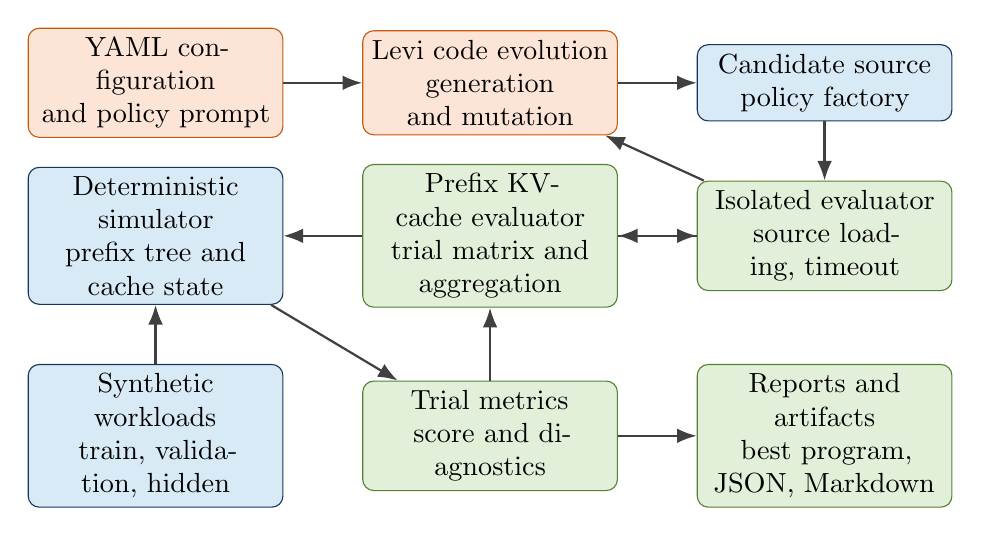
\begin{tikzpicture}[
  node distance=0.75cm and 1.0cm,
  box/.style={draw=navy, rounded corners, fill=lightblue, align=center,
              minimum height=0.8cm, text width=3.0cm},
  verify/.style={draw=green, rounded corners, fill=lightgreen, align=center,
                 minimum height=0.8cm, text width=3.0cm},
  search/.style={draw=orange, rounded corners, fill=lightorange, align=center,
                 minimum height=0.8cm, text width=3.0cm},
  arrow/.style={-{Latex[length=2.5mm]}, thick, draw=darkgray}
]
  \node[search] (config) {YAML configuration\\and policy prompt};
  \node[search, right=of config] (levi) {Levi code evolution\\generation and mutation};
  \node[box, right=of levi] (candidate) {Candidate source\\policy factory};

  \node[verify, below=of candidate] (entry) {Isolated evaluator\\source loading, timeout};
  \node[verify, left=of entry] (evaluator) {Prefix KV-cache evaluator\\trial matrix and aggregation};
  \node[box, left=of evaluator] (sim) {Deterministic simulator\\prefix tree and cache state};

  \node[box, below=of sim] (workloads) {Synthetic workloads\\train, validation, hidden};
  \node[verify, right=of workloads] (metrics) {Trial metrics\\score and diagnostics};
  \node[verify, right=of metrics] (artifacts) {Reports and artifacts\\best program, JSON, Markdown};

  \draw[arrow] (config) -- (levi);
  \draw[arrow] (levi) -- (candidate);
  \draw[arrow] (candidate) -- (entry);
  \draw[arrow] (entry) -- (evaluator);
  \draw[arrow] (evaluator) -- (sim);
  \draw[arrow] (workloads) -- (sim);
  \draw[arrow] (sim) -- (metrics);
  \draw[arrow] (metrics) -- (evaluator);
  \draw[arrow] (evaluator) -- (entry);
  \draw[arrow] (entry) -- (levi);
  \draw[arrow] (metrics) -- (artifacts);
\end{tikzpicture}
\caption{System-level data flow.  The candidate emits scores; the simulator owns all
state transitions.  The evaluator converts trial metrics into the scalar returned to
Levi while preserving detailed artifacts.}
\label{fig:architecture}
\end{figure}

\subsection{Relevant source files}

\begin{longtable}{>{\raggedright\arraybackslash}p{0.34\textwidth}
                  >{\raggedright\arraybackslash}p{0.60\textwidth}}
\toprule
\textbf{Path} & \textbf{Responsibility} \\
\midrule
\endhead
\filepath{src/prefix_cache_evolve/evaluators/prefix_kv_cache.py} &
Core data model, deterministic simulator, metrics, workloads, baselines, complexity
calculation, aggregation, and scoring. \\
\filepath{src/prefix_cache_evolve/problems/prefix_kv_cache/evaluator.py} &
Levi-facing isolated entry points for path, source, callable, and hidden evaluation. \\
\filepath{src/prefix_cache_evolve/problems/prefix_kv_cache/runner.py} &
CLI, evolution workflow construction, artifact persistence, baseline reports, hidden
reports, and plots. \\
\filepath{configs/prefix_kv_cache.yaml} &
Evolution prompt, model and pipeline configuration, workload panel, and score weights. \\
\filepath{src/prefix_cache_evolve/workflow/execution.py} &
Adapter between Levi's \code{evolve_code} API and the repository's evaluator result
format. \\
\filepath{src/prefix_cache_evolve/workflow/configuration.py} &
Pydantic-validated YAML loading and conversion into arguments forwarded to Levi. \\
\filepath{src/prefix_cache_evolve/problems/prefix_kv_cache/pressure_aware_incumbent.py} &
Current promoted deployable policy discovered by the 300-evaluation compact search. \\
\filepath{src/prefix_cache_evolve/problems/prefix_kv_cache/compact_seed.py} &
Prior compact incumbent retained as a small alternate evolution seed. \\
\filepath{scripts/tune_prefix_kv_compact.py} &
Reproducible coefficient sweep for the compact policy family. \\
\filepath{tests/test_prefix_kv_cache_evaluator.py} &
Functional PyTest coverage for policies, simulator invariants, metrics, workloads,
ranking behavior, reports, and evolution integration. \\
\bottomrule
\end{longtable}

\section{Candidate Contract and Trust Boundary}

\subsection{Required interface}

A candidate module must expose a compatible \code{build_candidate} or
\code{candidate_factory} factory.  The returned policy implements two scoring methods
and exactly three lifecycle callbacks:

\begin{lstlisting}[style=python]
def on_request_start(request: RequestInfo, now: int) -> None: ...
def on_cache_hit(block: PrefixBlockInfo, request: RequestInfo, now: int) -> None: ...
def on_cache_miss(block: PrefixBlockInfo, request: RequestInfo, now: int) -> None: ...

def score_admission(block: PrefixBlockInfo, now: int) -> float: ...
def score_eviction(block: PrefixBlockInfo, now: int) -> float: ...
\end{lstlisting}

Admission occurs only when \code{score_admission > 0}.  During eviction, the simulator
calls \code{score_eviction} for every legal victim and evicts the block with the
\emph{highest} score.  Therefore a high eviction score means ``evict sooner.''

\subsection{Candidate-visible request metadata}

\begin{tabularx}{\textwidth}{>{\ttfamily}p{0.31\textwidth} X}
\toprule
\normalfont\textbf{Field} & \textbf{Meaning} \\
\midrule
request\_id & Opaque per-trial request identifier.  It does not expose the sequential
generator index. \\
tenant\_id & Tenant namespace.  Prefix hashes include tenant identity, so cross-tenant
sharing is intentionally disabled. \\
session\_id & Request-only session metadata.  Blocks do not expose a session ID. \\
prompt\_length & Prompt length in tokens. \\
priority & Non-negative QoS signal.  It is not guaranteed to correlate with reuse. \\
request\_type & Normalized to the constant \code{request} before every candidate
callback.  Descriptive synthetic labels remain simulator-internal. \\
prompt\_tokens & Always replaced with an empty tuple before candidate callbacks,
including custom and trace-replay streams, preventing content fingerprinting. \\
predicted\_output\_length & Optional online estimate.  The true output length remains
simulator-internal. \\
recent\_admission\_pressure & Bounded 32-request online mean indicating how often prior
requests reached cache capacity.  It contains no workload-family label. \\
recent\_miss\_rate & Bounded 32-request online mean of prior per-request token miss
rates. \\
\bottomrule
\end{tabularx}

\subsection{Candidate-visible block metadata}

\begin{longtable}{>{\ttfamily}p{0.29\textwidth}
                  >{\raggedright\arraybackslash}p{0.65\textwidth}}
\toprule
\normalfont\textbf{Field} & \textbf{Meaning} \\
\midrule
\endhead
block\_id, prefix\_hash & Stable block key.  Candidate state should be keyed by one of
these values, never by Python object identity. \\
parent\_hash & Parent prefix block, or \code{None} for a root block. \\
depth & One-indexed block depth in the request prefix. \\
start\_token, end\_token, token\_count & Position and size of the block.  The final
block can be partial. \\
tenant\_id & Owning tenant. \\
created\_at, last\_accessed\_at & Logical arrival steps. \\
prev\_last\_accessed\_at & Previous observed prompt-chain access step, or \code{None}
before a prior access exists.  Online-computable from past and current arrivals. \\
last\_access\_gap & Logical-step distance from the current access to the previous
observed access, or \code{None} on first access. \\
access\_gap\_mean, access\_gap\_var & Fixed-state exponentially weighted first and
second-moment recurrence summary.  Both remain \code{None} until two gaps exist. \\
hit\_count & Historical hit count over the block's lifetime. \\
descendant\_count & Number of known descendant prefixes materialized so far. \\
active\_ref\_count & Number of active requests pinning the block. \\
subtree\_hit\_rate & Online hit rate aggregated over the block and all known
descendants. \\
subtree\_active\_ref\_count & Online active-reference total over the block and all known
descendants. \\
estimated\_recompute\_cost & Prefix-depth-sensitive deterministic recomputation cost. \\
\identifier{estimated_future_reuse}, \identifier{estimated_next_reuse_distance} &
\code{None} for deployable candidates; populated only for explicitly reporting-only
future-knowledge baselines. \\
\bottomrule
\end{longtable}

\subsection{Composable online primitives}

Candidates may optionally import \code{MultiTimescaleDecay}, \code{decay_vector}, and
\code{threshold_excess} from
\filepath{prefix_cache_evolve.problems.prefix_kv_cache.primitives}.
\code{MultiTimescaleDecay} maintains one to eight fixed-width exponential-decay
accumulators per key, bounds retained keys with deterministic least-recently-touched
eviction, and exposes \code{observe}, \code{observe_vector}, \code{values}, and
\code{combine}.  \code{observe} adds one amount to every channel, whereas
\code{observe_vector} adds a distinct amount per channel.  The latter lets a policy
represent bounded reuse, miss, or other online signals in one canonical state object
instead of hand-rolling several decay dictionaries.
\code{decay_vector} is the pure stateless counterpart.
\code{threshold_excess(value, threshold)} is a finite positive-hinge helper.  It was
added only after separate successful searches independently discovered persistent-
pressure and priority-aware pressure-excess terms.  It captures that repeated
functional form without constraining which online signal, threshold, coefficient, or
evidence interaction a policy may use.  These primitives expand the search space
without exposing future reuse or workload identity.

\subsection{What candidate code cannot control}

The simulator, not the policy, owns:

\begin{itemize}
  \item prefix hashing and prefix-tree structure;
  \item cache residency and capacity;
  \item active decode pins and release events;
  \item legal-victim filtering;
  \item admission rollback after pin-induced capacity failure;
  \item hit, miss, recompute, latency, churn, fairness, and audit accounting;
  \item hidden workload selection and future-knowledge audits.
\end{itemize}

Candidate methods returning non-numeric, boolean, infinite, or NaN scores are invalid.
Exceptions in factories, callbacks, or score functions also produce structured invalid
results.

\section{Simulator Design}

\subsection{Request and block construction}

Each workload produces a tuple of internal \code{WorkloadRequest} objects.  A request
contains candidate-visible \code{RequestInfo}, the simulator-only true output length,
the internal prompt tokens, and an optional logical arrival step.

The prompt is divided into physical cache blocks of \code{block_size_tokens}.  The
operative production-oriented default is sixteen tokens.  Synthetic traffic is
generated once at a fixed eight-token granularity, so block-size comparisons replay
identical token streams rather than changing prompt lengths with cache granularity.  For
each block depth \(d\), the simulator hashes the cumulative prefix:

\begin{equation}
  h_d = \operatorname{BLAKE2b}_{64}
        \left(\operatorname{repr}\left(
        \text{tenant\_id}, (t_1,\ldots,t_{\min(dB,L)})
        \right)\right),
\end{equation}

where \(B\) is the block size and \(L\) is prompt length.  Including the tenant ID
prevents accidental cross-tenant reuse.  Hashing the cumulative prefix rather than the
individual chunk ensures that identical chunks at different positions are not treated
as reusable prefix blocks.

The simulator materializes a rooted prefix tree lazily.  Internal block state includes
parent and child links, known descendant counts, global hit history, active reference
count, residency, and per-residency admission-accounting fields.

\subsection{Prefix-contiguous matching}

A request can reuse only the largest root-contiguous resident prefix.  Matching stops at
the first non-resident block:

\begin{equation}
  m(r) = \max\left\{k:
  b_1,\ldots,b_k \text{ are resident}\right\}.
\end{equation}

The simulator also enforces prefix-contiguous admission.  A block cannot be admitted
unless its parent is resident.  If admission is rejected or forced to bypass at depth
\(d\), deeper blocks remain misses and are not considered for admission.  This models
the reachability constraints of a real prefix cache rather than a generic unordered
object cache.

\subsection{Logical time and decode pinning}

The \code{now} argument is a logical arrival step, not wall-clock time.  Arrival steps
are monotonic but may repeat to model microbursts.  Requests without explicit arrival
steps default to sequential indices.

After a request begins, every hit or newly admitted block on its prefix is pinned for:

\begin{equation}
  D(r) = \max\left(1,
    \left\lceil\frac{\text{true output length}(r)}
                         {\text{active tokens per step}}\right\rceil
  \right).
\end{equation}

The default active generation rate is 64 tokens per logical step.  Release events
decrement active references when their logical time arrives.  Active blocks are never
legal eviction victims.  The candidate may see a predicted output length, but the true
length used for pinning is not exposed.

\paragraph{Optional shared prefix/decode capacity.}
The operative verifier remains in \code{prefix\_only} mode so historical selection
scores remain comparable.  An opt-in \code{shared} robustness mode additionally grows
decode KV at the configured active generation rate and charges it against the same
block capacity:

\begin{equation}
  N_{\text{prefix-resident}}(t) + N_{\text{decode-resident}}(t) \le C.
\end{equation}

Decode blocks are active and non-evictable.  New decode demand first evicts legal
inactive prefix leaves using the evaluated policy; if no legal prefix victim remains,
the simulator records failed decode-block allocations.  Failed demand is not retried,
but later demand continues to be measured, so any nonzero failure rate identifies an
infeasible demand trace rather than an executable schedule.  This makes the mode useful
for robustness analysis while leaving scheduler actions such as request rejection,
preemption, swapping, and separate prefix/decode budgets outside the current policy
surface.

\subsection{Per-request state machine}

\begin{figure}[H]
\centering
\resizebox{\textwidth}{!}{%
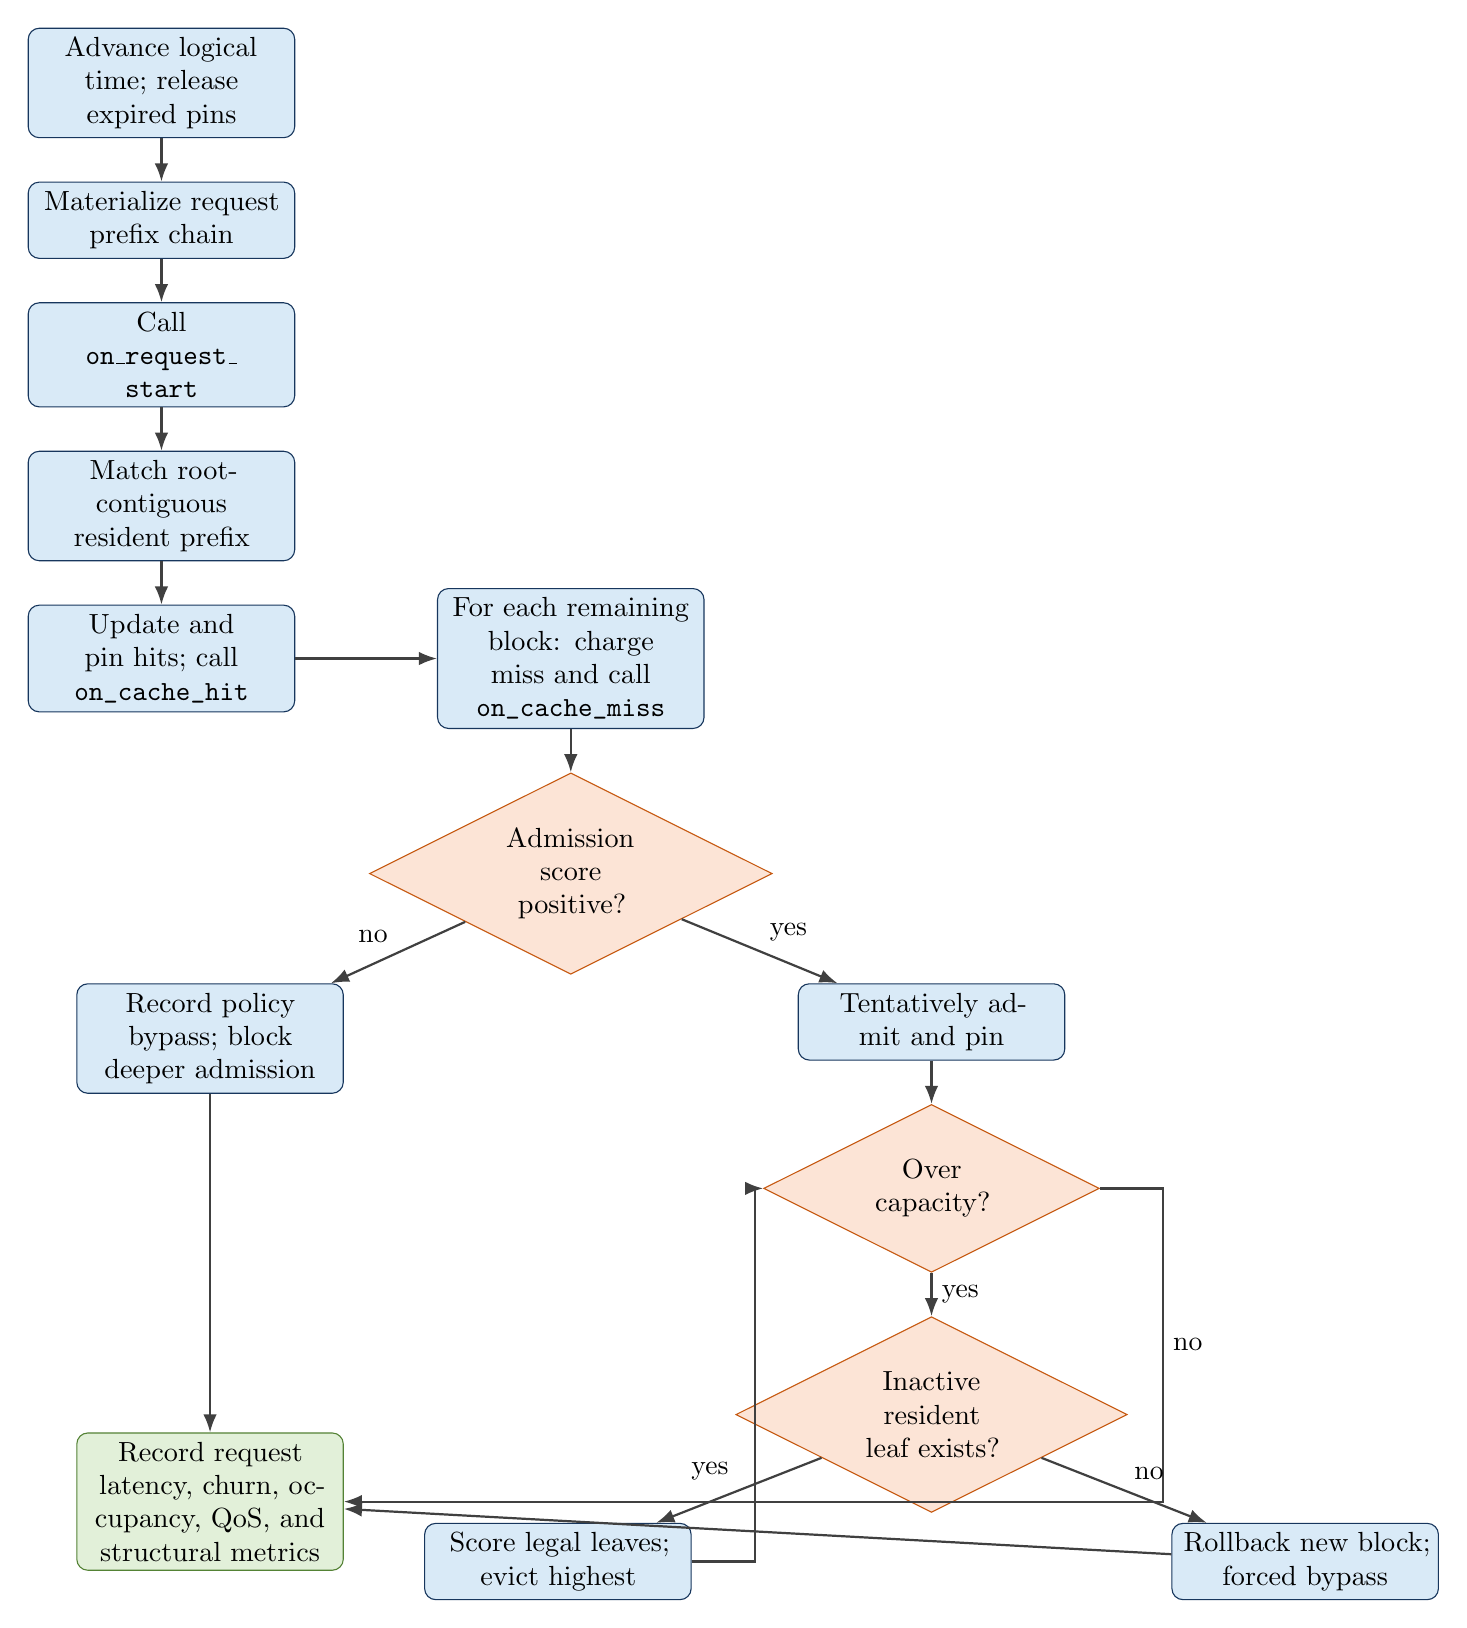
\begin{tikzpicture}[
  node distance=0.55cm and 0.75cm,
  state/.style={draw=navy, rounded corners, fill=lightblue, align=center,
                text width=3.15cm, minimum height=0.72cm},
  decision/.style={draw=orange, diamond, fill=lightorange, align=center,
                   aspect=2.0, text width=2.1cm},
  terminal/.style={draw=green, rounded corners, fill=lightgreen, align=center,
                   text width=3.15cm, minimum height=0.72cm},
  arrow/.style={-{Latex[length=2.3mm]}, thick, draw=darkgray}
]
  \node[state] (advance) {Advance logical time; release expired pins};
  \node[state, below=of advance] (materialize) {Materialize request prefix chain};
  \node[state, below=of materialize] (start) {Call\\{\ttfamily on\_request\_}\\
  {\ttfamily start}};
  \node[state, below=of start] (match) {Match root-contiguous resident prefix};
  \node[state, below=of match] (hits) {Update and pin hits; call\\\code{on_cache_hit}};
  \node[state, right=1.8cm of hits] (miss) {For each remaining block: charge miss and call
  \code{on_cache_miss}};
  \node[decision, below=of miss] (admitq) {Admission score positive?};
  \node[state, below left=0.75cm and 1.6cm of admitq] (bypass) {Record policy bypass;
  block deeper admission};
  \node[state, below right=0.75cm and 1.6cm of admitq] (tentative) {Tentatively admit and
  pin};
  \node[decision, below=of tentative] (over) {Over capacity?};
  \node[decision, below=of over] (victimq) {Inactive resident leaf exists?};
  \node[state, below left=0.75cm and 1.8cm of victimq] (evict) {Score legal leaves; evict
  highest};
  \node[state, below right=0.75cm and 1.8cm of victimq] (forced) {Rollback new block;
  forced bypass};
  \node[terminal, below=4.3cm of bypass] (record) {Record request latency, churn,
  occupancy, QoS, and structural metrics};

  \draw[arrow] (advance) -- (materialize);
  \draw[arrow] (materialize) -- (start);
  \draw[arrow] (start) -- (match);
  \draw[arrow] (match) -- (hits);
  \draw[arrow] (hits) -- (miss);
  \draw[arrow] (miss) -- (admitq);
  \draw[arrow] (admitq) -- node[above left]{no} (bypass);
  \draw[arrow] (admitq) -- node[above right]{yes} (tentative);
  \draw[arrow] (tentative) -- (over);
  \draw[arrow] (over) -- node[right]{yes} (victimq);
  \draw[arrow] (over.east) -- ++(0.8,0) |- node[pos=0.25,right]{no} (record.east);
  \draw[arrow] (victimq) -- node[above left]{yes} (evict);
  \draw[arrow] (evict.east) -- ++(0.8,0) |- (over.west);
  \draw[arrow] (victimq) -- node[above right]{no} (forced);
  \draw[arrow] (bypass) -- (record);
  \draw[arrow] (forced) -- (record);
\end{tikzpicture}
}
\caption{Per-request simulator flow.  Miss callbacks continue for the remaining chain
even after admission becomes blocked, but deeper blocks are not scored for admission.}
\label{fig:request-flow}
\end{figure}

\subsection{Admission semantics}

For the first missed block whose parent path is still admissible:

\begin{enumerate}
  \item The simulator calls \code{score_admission}.
  \item A score at or below zero rejects the block, records deliberate policy bypass,
  and prevents deeper admission.
  \item A positive score tentatively makes the block resident and pins it.
  \item If capacity is exceeded, the simulator repeatedly evicts legal victims.
  \item If no legal victim exists because all leaves are pinned, the tentative block is
  rolled back and the rest of the request is forced to bypass.
\end{enumerate}

The newly admitted block is pinned before victim selection and therefore cannot
immediately evict itself.  An admission can evict one or more blocks and still fail if
the remaining over-capacity state has no legal victim.  The verifier counts those
evictions in churn and latency even though the new block is rolled back.

\subsection{Eviction legality}

Only inactive resident leaves are legal victims.  Interior nodes cannot be evicted
because doing so would make resident descendants unreachable.  Active leaves cannot be
evicted because an ongoing decode references them.

The legal set at time \(t\) is:

\begin{equation}
  \mathcal{V}_t =
  \left\{b:
  b.\text{resident}
  \land b.\text{resident\_children}=\varnothing
  \land b.\text{active\_ref\_count}=0
  \right\}.
\end{equation}

The simulator computes the policy score for every \(b\in\mathcal{V}_t\) and evicts:

\begin{equation}
  b^\star = \arg\max_{b\in\mathcal{V}_t}
             \operatorname{score\_eviction}(b,t).
\end{equation}

\subsection{Cost and latency proxy}

The estimated recomputation cost of a block is depth-sensitive:

\begin{equation}
  c(b) = b.\text{end\_token}\cdot c_{\text{prefill-token}},
\end{equation}

with \(c_{\text{prefill-token}}=1\) by default.  Summing this value across missed blocks
approximates the growing attention cost of recomputing progressively deeper prefixes.

For a request \(r\), the deterministic latency proxy is:

\begin{equation}
  \ell(r) =
  \sum_{b\in\text{misses}(r)} c(b)
  + 0.035\cdot\text{lookup blocks}(r)
  + 0.2\cdot\text{evictions}(r).
\end{equation}

A lookup probes all matched blocks and one failed block when the full prefix is not
resident.  The simulator reports p50, p95, and p99 latency proxies, high-priority tail
latency, recovery-phase latency, and p95 recompute cost.

\subsection{Useful and wasted admission accounting}
\label{sec:admission-accounting}

Admission quality is tracked per \emph{residency interval}, not per globally known
block.  Internal state contains:

\begin{lstlisting}[style=python]
admission_tracked: bool
resident_hit_count: int
\end{lstlisting}

When a block is tentatively made resident, these fields reset.  The interval becomes
tracked only after the block survives capacity enforcement.  Each later cache hit while
resident increments \code{resident_hit_count}.  The miss that caused the admission is
not a hit.

When a tracked block is evicted, or when the trial ends while it remains resident:

\begin{align}
  \text{useful admission} &\iff \text{resident hit count} > 0,\\
  \text{wasted admission} &\iff \text{resident hit count} = 0.
\end{align}

Rejected and forced-bypass attempts are neither useful nor wasted admissions because
they never became successful admissions.  If a block is admitted, evicted, and later
admitted again, the two intervals are classified independently.

The binary rates are:

\begin{equation}
  A_{\text{useful}} =
  \frac{N_{\text{useful}}}{\max(1,N_{\text{admitted}})},\qquad
  A_{\text{wasted}} =
  \frac{N_{\text{wasted}}}{\max(1,N_{\text{admitted}})}.
\end{equation}

For nonzero admissions the rates sum to one.  The verifier also reports
\metric{evicted_without_hit_rate}, which narrows the waste metric to admissions evicted
without an intervening hit.

The binary classification is retained for interpretation, but the verifier now also
weights admission outcomes by block token count.  For successful residency intervals
\(i\), let \(s_i\) be the block's token count and \(h_i\) its resident hit count:

\begin{align}
  T_{\text{admitted}} &= \sum_i s_i,\\
  T_{\text{useful}} &= \sum_{i:h_i>0}s_i,\qquad
  T_{\text{wasted}} = \sum_{i:h_i=0}s_i,\\
  T_{\text{saved-by-admission}} &= \sum_i h_i s_i.
\end{align}

The token-weighted waste rate is
\(T_{\text{wasted}}/\max(1,T_{\text{admitted}})\).  It is the admission-waste
quantity used by the score, so wasting a full block costs more than wasting a partial
block.  Realized admission utility is reported as:

\begin{equation}
  U_{\text{admission-token}} =
  \frac{T_{\text{saved-by-admission}}}
       {\max(1,N_{\text{admitted}}B)},
\end{equation}

where \(B\) is the configured block size.  This is the average number of full-block
equivalent token reuses delivered per successful admitted cache slot.  It distinguishes
a one-hit full block from a one-hit partial block and credits repeated hits.  The score
adds a small concave \(\log(1+U_{\text{admission-token}})\) reward, which makes the
metric actionable without double-counting saved tokens linearly.

\subsection{Verifier-only future audits}

The simulator maintains two future-reuse trackers:

\begin{itemize}
  \item The \textbf{candidate-visible tracker} is disabled for deployable candidates and
  enabled only for reporting-only future-reuse baselines.
  \item The \textbf{audit tracker} is always enabled internally, but its information is
  never included in candidate-visible block metadata.
\end{itemize}

The audit tracker supports \emph{avoidable eviction} accounting.  At each eviction, the
verifier compares the selected victim's next-use distance with every other legal
victim.  The eviction is avoidable if another legal victim would be reused later:

\begin{equation}
  E_{\text{avoidable}} =
  \mathbf{1}\left[
  d_{\text{next}}(b^\star)
  < \max_{b\in\mathcal{V}_t\setminus\{b^\star\}}
      d_{\text{next}}(b)
  \right].
\end{equation}

This is a regret diagnostic, not an oracle instruction to the policy.  A
short-reuse avoidable eviction is additionally recorded when the selected victim is
reused within eight logical steps while an alternative is reused later than eight
steps.  The constrained next-use oracle has zero avoidable evictions by construction.

The same boundary prevents indirect workload reconstruction.  Workload generation uses
family-specific random seeds internally, while every candidate factory receives the
separate fixed \code{policy_seed} value.  Candidate-visible request IDs are opaque,
synthetic request-type labels are normalized to \code{request}, and prompt-token
content is scrubbed before every callback.  Registered baselines cannot be marked both
deployable and future-reuse-dependent.

This is an experimental trust boundary, not an adversarial Python security sandbox.
Candidate source executes in an isolated process, but arbitrary malicious Python could
attempt reflection or inspect local source and artifacts.  Reported searches therefore
also retain static source checks and source audit; a capability-isolated policy process
or restricted DSL would be required for security against deliberately evasive code.

\section{Workload Model}

\subsection{Trial matrix and split policy}

The discovery full panel used 96 requests per workload, seeds \((11,23,37)\), block
size eight, and capacities \((48,96)\).  The operative production-oriented panel uses
block size sixteen and capacities \((24,48)\), preserving the same
\((384,768)\)-token capacity tiers.  A separate robustness report replays identical
token streams with block sizes \(8\), \(16\), and \(32\).

All headline numbers use synthetic streams generated from committed source; no private
or external production trace contributes to them.  The exact historical evaluator
settings are retained in
\filepath{configs/prefix_kv_cache_discovery.yaml}.  The committed discovery workload
manifest records summaries and SHA-256 fingerprints for all 81 ordered synthetic
streams, plus the generator-source hash and CPython version.  Its aggregate
access-pattern fingerprint starts \identifier{4607782d2315}; the manifest retains
the full value.
Production-trace replay remains a separate user-supplied path; trace reports record the
input-file hash, and replay reports also record the derived request-stream hash.

On that robustness panel, the incumbent scores \(62.757\) at the primary
16-token size, narrowly behind TinyLFU+LRU at \(63.548\) after the incumbent's
\(8.232\) complexity charge.  Its raw pre-complexity score is \(70.989\), with
higher validation token hit (\(0.598\) versus \(0.580\)) and lower churn
(\(168.1\) versus \(499.0\)).  At 32 tokens the incumbent ranks first among the
compared policies, but all combined scores are negative; the coarse block size
substantially damages irregular-prefix reuse.

\begin{center}
\begin{tabular}{lrrrr}
\toprule
\textbf{Split} & \textbf{Families} & \textbf{Capacities} & \textbf{Seeds} &
\textbf{Trials} \\
\midrule
Train & 5 & 2 & 3 & 30 \\
Validation selection & 10 & 2 & 3 & 60 \\
Structure-generalization probe & 2 & 2 & 3 & 12 \\
Normal evaluation, including probe & 17 & 2 & 3 & 102 \\
Hidden final report & 10 & 2 & 3 & 60 \\
\bottomrule
\end{tabular}
\end{center}

Each family receives a deterministic seed offset of \(1000(i+1)\), where \(i\) is its
position within its split.  The main combined score uses validation trials only.
Training metrics are emitted for diagnosis and prompt context.  Probe metrics are
reported during normal evaluation but excluded from the combined score, success flag,
and invalidity surcharge.  Hidden metrics are quarantined behind a separate evaluator
entry point.

The \code{--quick} mode uses 36 requests and seed \((3,)\).  It is intentionally labeled
smoke-only because prior runs demonstrated that a single-seed slice can materially
misrank the field.

\subsection{Workload families}

\begin{longtable}{>{\raggedright\arraybackslash}p{0.24\textwidth}
                  >{\raggedright\arraybackslash}p{0.11\textwidth}
                  >{\raggedright\arraybackslash}p{0.57\textwidth}}
\toprule
\textbf{Family} & \textbf{Default split} & \textbf{Behavior and failure mode exposed} \\
\midrule
\endhead
\identifier{shared_system_prompt} & Train &
Repeated shared system instructions, a small recurring task set, and request-specific
tails.  Rewards preservation of shallow broadly shared roots. \\
\identifier{rag_template_reuse} & Train &
Shared RAG template, position-stable recurring chunks, and query tails.  Avoids
incorrectly crediting arbitrary repeated chunks outside prefix alignment. \\
\identifier{long_context_mixed} & Train &
Recurring documents with varying prefix depths and partial tails.  Stresses
depth-sensitive recomputation value. \\
\identifier{session_continuation_growth} & Train &
Interleaved conversations that grow by one turn per revisit.  Stresses paused deep
history preservation. \\
\identifier{agentic_tool_workflows} & Train &
Six interleaved tool-using workflows fork from shared checkpoints, resume paused
routes, append variable multi-step observations, and periodically replan after a
rollback.  Trains irregular agentic reuse without duplicating the held-out probe. \\
\midrule
\identifier{agent_trace_branching} & Probe &
Shared agent roots and schemas with accumulating tool history, branches, and retries.
Tests trunks, fanout, deep histories, and rollback-like retry behavior. \\
\identifier{phase_shift_prompts} & Validation &
Popular prompt family changes halfway through the run.  Exposes stale-history
overprotection. \\
\identifier{multi_tenant_skew} & Validation &
Uneven tenant volume with tenant-specific roots.  Supplies the score's explicit
max--min tenant fairness penalty. \\
\identifier{hotset_cold_scan} & Validation &
Warm hot set, one-off scan, then hot-set return.  Tests pollution resistance and
recovery. \\
\identifier{cyclic_working_set_pressure} & Probe &
Repeatedly traverses working sets near and beyond cache capacity, then expands the
cycle.  Exposes short-horizon and avoidable eviction regret. \\
\identifier{concurrent_long_generation} & Validation &
Batched arrivals and long outputs create overlapping pins and forced-bypass pressure. \\
\identifier{reasoning_burst} & Selectable robustness &
Three-request microbursts combine recurring prefixes, noisy predicted output lengths,
and heavy-tailed reasoning outputs. \\
\identifier{reasoning_burst_shifted} & Selectable robustness &
Four-request microbursts with longer reasoning outputs and a shifted branch traversal. \\
\identifier{stochastic_serving_mix} & Validation &
Interleaves chat, RAG, agent, long-generation, and one-off traffic under changing
regimes, bursts, and arrival gaps. \\
\identifier{rolling_template_versions} & Validation &
Stable version, canary overlap, majority rollout, and rollback.  Tests stale-version
retirement and active-version warmth. \\
\identifier{heavy_tailed_prefix_lengths} & Validation &
Recurring documents with Pareto-like prefix depths.  Tests expensive long-tail
contexts. \\
\identifier{priority_burst_recovery} & Validation &
Recurring high-priority traffic before, during, and after low-priority scan pollution.
Rewards appropriate priority protection and recovery. \\
\identifier{priority_one_off_noise} & Validation &
Reusable normal-priority traffic competes with mostly unique high-priority requests.
Prevents learning that priority automatically implies reuse. \\
\midrule
\identifier{adversarial_unique_prompts} & Hidden &
Mostly unique prompts.  Exposes admit-everything churn and dead admissions. \\
\identifier{cross_family_mixture} & Hidden &
Mixture of shared, phase-shifted, and unique requests. \\
\identifier{tenant_session_reentry} & Hidden &
Paused tenant sessions reenter after unrelated traffic with new one-off tails. \\
\identifier{stochastic_serving_mix_shifted} & Hidden &
More bursty, more one-off, and different regime weights. \\
\identifier{rolling_template_versions_shifted} & Hidden &
Rolls forward to a new version with a changed root. \\
\identifier{heavy_tailed_prefix_lengths_shifted} & Hidden &
Heavier tail, more documents, and deeper maximum prefix. \\
\identifier{priority_burst_recovery_shifted} & Hidden &
Higher priority range, larger hot set, deeper scans, and stronger burst pressure. \\
\identifier{cyclic_working_set_pressure_shifted} & Hidden &
Larger cycles and a different traversal stride. \\
\identifier{priority_one_off_noise_shifted} & Hidden &
Higher one-off priority burst ratio and deeper one-off prompts. \\
\identifier{tenant_phase_shift_cycles_shifted} & Hidden &
Longer tenant phases, repeated pollution/recovery cycles, and larger delayed reentry
gaps. \\
\bottomrule
\end{longtable}

\section{Verifier and Metrics}

\subsection{Metric taxonomy}

The verifier emits metrics at trial, split, workload, and capacity aggregation levels.
Important categories include:

\begin{itemize}
  \item \textbf{Reuse:} token and block hit rate, saved prefill tokens, depth-band hit
  rates, role-specific hit contributions.
  \item \textbf{Request service:} per-request p10 and p50 hit rates, worst-quarter and
  final-quarter token hit, quarter-to-quarter variance.
  \item \textbf{QoS:} priority-weighted hit rate, high- and low-priority hit rates,
  high-priority p10 request hit and tail latency.
  \item \textbf{Admission:} attempts, successful admissions, rejections, policy bypass,
  forced bypass, binary useful/wasted admissions, admitted/useful/wasted token mass,
  saved tokens per admitted slot, policy-caused underfill, and evictions without a hit.
  \item \textbf{Eviction regret:} reuse after eviction, short-distance reuse misses,
  reuse-distance percentiles, avoidable evictions, and avoidable short-reuse
  evictions.
  \item \textbf{Cost and pressure:} recompute tokens and cost, lookup probes, p50/p95/p99
  latency proxy, churn per 1000 requests, total/prefix/decode occupancy, decode-block
  demand, allocation failures, decode-pressure evictions, active-request peak, and
  maximum prefill cost.
  \item \textbf{Fairness:} tenant max--min hit-rate gap, tenant p10 hit rate, and Jain
  fairness.
  \item \textbf{Robustness aggregation:} worst trial, p10 across trials, and
  cross-trial standard deviation.
  \item \textbf{Validity and complexity:} invalid reason/fraction, timeout and memory
  failures, and scoring-function AST complexity.
\end{itemize}

\subsection{Workload-capacity base score}

For one workload-capacity group \(G\), containing three seed trials, define:

\begin{align}
  B(G) ={}&
  80\,\overline{H_{\text{tok}}}
  +60\,\overline{H_{\text{blk}}}
  +12\,\overline{H_{\text{req,p10}}}
  +12\,\overline{H_{\text{worst-quarter}}} \nonumber\\
  &+8\,\overline{H_{\text{high-priority}}}
  +\overline{\log(1+U_{\text{admission-token}})}
  -6\,\overline{A_{\text{wasted,tok}}}
  -8\,\overline{E_{\text{avoidable}}}
  -C_{\text{latency}}(G).
\end{align}

The priority term is included only for groups that contain positive-priority requests.
The automatic latency normalizer is scoped to the same workload-capacity group:

\begin{align}
  L_{\text{norm}}(G) &=
  \max_{i\in G}\text{max-prefill-cost}_i,\\
  C_{\text{latency}}(G) &=
  \min\left(40,\,
    35\frac{\overline{\text{p95-latency}}}{\max(1,L_{\text{norm}}(G))}
  \right).
\end{align}

This scoping prevents a long-context family from making latency penalties negligible
for all shorter workloads.

\subsection{Worst-seed blending}

For workload-capacity group \(G\), the verifier computes the group-average base score
and the minimum single-seed base score:

\begin{equation}
  S_G = 0.85\,B(G) + 0.15\min_{i\in G}B(\{i\}).
\end{equation}

This retains a strong mean signal while charging policies whose performance collapses
on one seed.

\subsection{Combined score}

For trial \(i\), policy-caused underfill multiplies deliberate policy bypass by unused
mean capacity:

\begin{equation}
  U_i =
  \text{policy-bypass-token-rate}_i
  \max\left(0,1-\frac{\text{mean-prefix-occupancy}_i}{\text{capacity}_i}\right).
\end{equation}

This distinguishes a selective policy that leaves reusable cache space idle from
natural underfill on short or low-reuse workloads where every miss is admitted.  Decode
occupancy is deliberately excluded so active generation cannot mask a prefix policy
that bypasses useful admissions.

Let \(\mathcal{G}\) be the 20 validation workload-capacity groups.  Let
\(\overline{\chi}\) be mean validation churn per 1000 requests, \(\overline{U}\) be
mean validation policy-caused underfill, \(F\) be mean tenant max--min gap on
\code{multi_tenant_skew}, and \(C\) be candidate AST complexity.  The combined score
is:

\begin{align}
  S_{\text{combined}} ={}&
  \frac{1}{|\mathcal{G}|}\sum_{G\in\mathcal{G}} S_G
  +0.5\min_{G\in\mathcal{G}}S_G \nonumber\\
  &-\min(25,0.015\,\overline{\chi})
  -\min(15,12\,\overline{U})
  -\min(30,80F)
  -0.065\,C^{0.75}.
\end{align}

The weakest-workload contribution can be negative.  This is intentional: catastrophic
behavior on one workload-capacity pair should reduce the total even if the mean is
strong.

\subsection{Complexity accounting}

Legacy complexity is the number of Python AST nodes in candidate implementation classes
and functions.  Thin factory wrappers named \code{build_candidate},
\code{candidate_factory}, or \code{run_demo} are ignored, but nested implementations
inside them are counted.  A syntax error receives complexity 10,000 before failing
loading.

The current configuration enables form-aware complexity.  Each statically recognized
call site using \code{MultiTimescaleDecay} or \code{decay_vector} from the canonical
primitive module receives a three-node credit.  The smaller
\code{threshold_excess} helper receives one node, because its hidden implementation is
only a positive hinge rather than bounded state machinery.  Total credit is capped at
25\% of raw implementation nodes.  The cap prevents primitive calls from making
arbitrary code free; repeated dead calls still increase effective complexity.  Setting
\code{form_aware_complexity: false} restores the legacy raw-node schedule.

The penalty \(0.065C^{0.75}\) is:

\begin{itemize}
  \item \textbf{unbounded}, so large dead implementations never become free;
  \item \textbf{concave}, so necessary implementation detail is not charged linearly;
  \item \textbf{behavior-independent}, allowing complexity to break near-ties between
  policies with similar outcomes.
  \item \textbf{form-aware but bounded}, mildly favoring reusable online primitives
  without suppressing the cost of custom control flow or state.
\end{itemize}

The penalty remains smooth and unbounded, but search also uses separate safety and
promotion limits.  The general lane rejects candidates above 650 effective nodes.
The eviction-specialist lane exposes only a victim-ranking function and explores up
to 1000 effective nodes so richer eviction ideas can be measured.  Search ranks raw
behavior before complexity, preventing deletion alone from appearing as progress.
Final promotion composes the function into the complete incumbent and retains 650 as
the deployable-source limit.  Thus the safety limit controls evaluation cost and
pathological growth, while the promotion limit controls deployability.

\subsection{Invalid candidates, isolation, and memory}

Candidate evaluation runs in an isolated worker with the operative YAML timeout of
90 seconds.  Candidate memory is monitored with \code{tracemalloc}; the default peak
limit is 64 MiB.

Any positive invalid fraction bypasses normal scoring:

\begin{equation}
  S_{\text{invalid}} =
  -1000 - 1 - 1000\,f_{\text{invalid}}.
\end{equation}

This keeps invalid programs below representative valid programs even when the valid
program is very complex.

\subsection{Baseline and oracle policies}

\begin{longtable}{>{\ttfamily}p{0.24\textwidth}
                  >{\raggedright\arraybackslash}p{0.16\textwidth}
                  >{\raggedright\arraybackslash}p{0.52\textwidth}}
\toprule
\normalfont\textbf{Policy} & \textbf{Class} & \textbf{Purpose} \\
\midrule
\endhead
\identifier{no_cache} & Deployable & Lower bound and bypass sanity check. \\
lru & Deployable & Recency baseline; evicts least recently used legal leaf. \\
\identifier{sglang_radix_attention} & Deployable & SGLang RadixAttention's default
radix-cache replacement policy; retains cache-page-aligned prefixes and recursively
evicts the least-recently-used unreferenced leaf.  Registered as a selectable
reference but excluded from default comparisons because it maps to leaf-LRU here. \\
\identifier{vllm_apc} & Deployable & Production-style vLLM APC baseline; caches only
full blocks and uses LRU with deepest-prefix tie-breaking among legal victims. \\
lfu & Deployable & Frequency baseline with LRU tie-breaking. \\
\identifier{depth_prefer_shallow} & Deployable & Protects shallow roots. \\
\identifier{recompute_greedy} & Deployable & Protects expensive-to-recompute prefixes. \\
\identifier{cost_aware_lru} & Deployable & Blends recency and recomputation cost. \\
\identifier{prefix_fanout} & Deployable & Protects prefixes with known descendants. \\
\identifier{prefix_anchor} & Deployable & Structural anchor heuristic. \\
\identifier{tinylfu_lru} & Deployable & Selective admission with LRU-style eviction. \\
\identifier{tenant_fair_lru} & Deployable & Biases eviction toward better-served tenants. \\
\identifier{future_reuse_heuristic} & Reporting only & Uses future reuse count and next distance;
not an upper bound. \\
\identifier{oracle_future_reuse} & Reporting only & Rejects blocks with no future reuse and evicts
the legal victim whose next use is furthest away.  It is constrained by the simulator's
prefix-tree, leaf-only, and pinning rules. \\
\bottomrule
\end{longtable}

\section{State of the Art in KV-Cache Management}
\label{sec:state-of-the-art}

\subsection{There is no single ``best KV-cache algorithm''}

As of June 5, 2026, KV-cache research covers several different optimization problems
that are often reported under the same name.  Their headline speedups are not directly
comparable: papers use different models, hardware, context lengths, quality constraints,
arrival processes, baselines, and definitions of cache capacity.  A system that moves
KV tensors efficiently from SSD solves a different problem from a policy that decides
which exact-prefix block to evict from GPU memory.

The following taxonomy separates those problems before comparing their techniques:

\begin{longtable}{>{\raggedright\arraybackslash}p{0.19\textwidth}
                  >{\raggedright\arraybackslash}p{0.27\textwidth}
                  >{\raggedright\arraybackslash}p{0.25\textwidth}
                  >{\raggedright\arraybackslash}p{0.19\textwidth}}
\toprule
\textbf{Problem class} & \textbf{Representative systems} & \textbf{Primary decision}
& \textbf{Relation to this simulator} \\
\midrule
\endhead
Exact cross-request prefix reuse &
vLLM APC, SGLang RadixAttention, SAECache \cite{vllm-apc,sglang,saecache} &
Which lossless, exactly reusable prefix blocks remain in a finite accelerator cache? &
Directly in scope. \\
Workflow-aware prefix reuse &
KVFlow, INFERCEPT \cite{kvflow,infercept} &
Which paused or soon-to-run agent state should be retained, swapped, or prefetched? &
Partially modeled; workflow schedules and prefetch are absent. \\
Distributed and tiered caching &
Preble, Mooncake, MemServe, LMCache, Tutti
\cite{preble,mooncake,memserve,lmcache,tutti} &
Where should a request run, and where should its KV state live across GPU, CPU, network,
and SSD tiers? &
Out of scope for the current single-cache simulator. \\
Non-prefix and RAG reuse &
Prompt Cache, RAGCache, CacheBlend \cite{promptcache,ragcache,cacheblend} &
How can reusable modules or retrieved chunks be reused when they are not one
root-contiguous prefix? &
Out of scope; the simulator intentionally requires exact prefix contiguity. \\
Within-request KV reduction &
H2O, KIVI, SnapKV, Quest, LaProx, VeriCache
\cite{h2o,kivi,snapkv,quest,laprox,vericache} &
Which tokens, pages, layers, or tensor bits are needed while decoding one long request? &
A separate problem; it requires model-quality and attention-kernel simulation. \\
\bottomrule
\end{longtable}

For the current project, the most relevant comparison set is the first row.  The other
rows are important because they identify the next simulator dimensions, but they should
not be mixed into the current prefix-policy leaderboard.

\subsection{Production reference designs: PagedAttention, APC, and RadixAttention}

\paragraph{PagedAttention and block-based allocation.}
PagedAttention introduced operating-system-style paging for KV memory and flexible
sharing of non-contiguous physical blocks.  It substantially reduces fragmentation and
duplication, enabling larger batches and shared KV state, but it is primarily a memory
layout and allocation mechanism rather than a value-aware replacement policy
\cite{pagedattention}.  The current simulator assumes that a fixed-size block abstraction
already exists; it evaluates the policy layer built on top of that abstraction.

\paragraph{vLLM Automatic Prefix Caching.}
Current vLLM APC identifies a block by hashing its tokens together with its complete
prefix.  Only blocks with reference count zero are evictable.  The production policy
uses LRU, with deeper blocks preferred for eviction when last-access times tie
\cite{vllm-apc}.  This design preserves common ancestors and is equivalent in effect to
RadixAttention's leaf-first LRU for full-attention models.

\paragraph{SGLang RadixAttention.}
RadixAttention stores reusable KV state in a radix tree, evicts the least-recently-used
leaf first, and protects nodes referenced by running requests
\cite{sglang}.  SGLang couples this cache with cache-aware scheduling and reported up to
\(6.4\times\) higher throughput than its evaluated serving baselines across structured
LLM-program workloads.  The simulator closely models RadixAttention's replacement
constraints: root-contiguous matching, leaf-only eviction, active-reference pinning,
and common-ancestor preservation.  It does not yet model the scheduler or continuous
batching effects that contribute to end-to-end SGLang performance.
The simulator treats every modeled block-tree node as a cacheable radix unit, so the
explicit \identifier{sglang_radix_attention} baseline is behaviorally equivalent to
generic leaf-LRU under this contract.  It remains visible in documentation and as an
interactive-lab option, but default comparisons exclude the duplicate row.  The
implementation mapping was checked against pinned SGLang commit
\href{https://github.com/sgl-project/sglang/tree/52f221cce088abc998fa9d3812416a45ee0e2e25/python/sglang/srt/mem_cache}{52f221cce088abc998fa9d3812416a45ee0e2e25}.
This remains a block-tree approximation: simulator capacity is charged in fixed
blocks rather than SGLang's token/page-counted radix nodes.

\paragraph{Practical conclusion.}
The production reference remains structurally constrained LRU, not a large
hand-engineered scoring function.  This is an important benchmark property: any evolved
policy should beat exact APC/Radix-style LRU by enough to justify its extra state,
scoring work, and operational complexity.

\subsection{Strongest directly relevant research policies}

\paragraph{SAECache: semantic-adaptive prefix eviction.}
The most directly relevant recent research result is SAECache, a May 2026 preprint
focused specifically on prefix-cache eviction \cite{saecache}.  Its central observation
is that blocks associated with system prompts, user queries, tool output, model
responses, and reasoning traces have very different reuse distributions.  It combines:

\begin{itemize}
  \item task-specific queues for session reuse and structural/template reuse;
  \item semantic-aware token weighting learned from eviction feedback;
  \item online adaptation of timing distributions, position decay, queue weights, and
  meta-parameters.
\end{itemize}

SAECache reports \(1.4\times\)--\(2.7\times\) TTFT improvement over production-style
baselines on its evaluated heterogeneous workloads.  It also reports that fixed
parameters can degrade by as much as \(2.7\times\) under workload mismatch.  The second
result is particularly relevant here: it supports the verifier's phase-shift, shifted
hidden families, and complexity pressure, and it argues for online adaptation rather
than a permanently tuned coefficient vector.

The current candidate cannot reproduce SAECache faithfully.  Prompt tokens are hidden,
blocks do not expose generic semantic roles, and the candidate contract has no eviction
feedback callback.  Adding those signals must preserve the trust boundary: expose
deployable generic roles such as system, user, tool, assistant, retrieved document, and
unknown, rather than exposing workload-family names or future reuse.

\paragraph{KVFlow: workflow-aware agent caching.}
KVFlow targets multi-agent workflows and represents the known execution plan as an Agent
Step Graph \cite{kvflow}.  A steps-to-execution signal guides fine-grained KV-node
eviction, while background prefetch overlaps CPU-to-GPU transfer for agents expected to
run next.  It reports up to \(1.83\times\) speedup for single large-prompt workflows and
\(2.19\times\) for concurrent workflows relative to SGLang with a hierarchical radix
cache.

This is not future leakage when the workflow graph is genuinely known to the serving
system.  It is deployable application metadata.  The current
\identifier{agent_trace_branching} workload models shared roots, branches, and retries,
but it does not expose a declared workflow graph, cache tiers, or prefetch overlap.
Consequently, the evaluator can test generic reuse learning but not KVFlow's central
algorithm.

\subsection{Systems that expand the effective cache}

Several leading systems improve KV reuse less by inventing a better single-GPU victim
score and more by changing placement, routing, or storage:

\begin{longtable}{>{\raggedright\arraybackslash}p{0.16\textwidth}
                  >{\raggedright\arraybackslash}p{0.37\textwidth}
                  >{\raggedright\arraybackslash}p{0.19\textwidth}
                  >{\raggedright\arraybackslash}p{0.17\textwidth}}
\toprule
\textbf{System} & \textbf{Core algorithmic contribution} &
\textbf{Paper-reported result} & \textbf{Missing simulator capability} \\
\midrule
\endhead
Preble &
Jointly schedules requests and prefixes across GPUs using exploitation versus
exploration, prompt-sharing features, load, and recomputation cost
\cite{preble}. &
\(1.5\times\)--\(14.5\times\) lower average latency and \(2\times\)--\(10\times\)
lower p99 latency than evaluated systems. &
Multiple workers, routing, queueing, replication, load. \\
Mooncake &
Disaggregates prefill and decode, uses GPU-cluster CPU/DRAM/SSD as a KV cache, and
schedules for effective throughput under SLOs \cite{mooncake}. &
Kimi handled 75\% more requests under reported real workloads. &
SLOs, overload rejection, prefill/decode clusters, tiers. \\
LMCache &
Provides a cache layer and control API across GPU, CPU, storage, network, engines, and
queries; pipelines and batches KV movement \cite{lmcache}. &
Up to \(15\times\) throughput improvement with vLLM in evaluated workloads. &
Bytes, transfer bandwidth, remote lookup, overlap, connectors. \\
Tutti &
Uses a GPU-centric KV object store and GPU-driven asynchronous SSD I/O with
slack-aware scheduling \cite{tutti}. &
78.3\% lower TTFT and \(2\times\) achievable request rate versus evaluated
GDS-backed SSD LMCache. &
SSD objects, I/O queues, GPU/CPU contention, slack. \\
\bottomrule
\end{longtable}

These results indicate that the globally best serving decision is often joint:
\emph{admission, eviction, tier placement, prefetch, and request routing}.  A
single-cache score can still be valuable, but the next major simulator expansion should
make transfer and placement first-class decisions.

\subsection{Beyond exact prefixes}

Exact-prefix reuse is lossless and simple, but it leaves substantial value unused in
RAG and modular prompts:

\begin{itemize}
  \item \textbf{Prompt Cache} explicitly declares reusable prompt modules and preserves
  positional correctness when those modules appear in prompts \cite{promptcache}.
  \item \textbf{RAGCache} stores retrieved knowledge states in a GPU/host knowledge tree
  and uses a RAG-aware replacement policy; it reports up to \(4\times\) lower TTFT and
  \(2.1\times\) throughput versus its evaluated vLLM--Faiss baseline
  \cite{ragcache}.
  \item \textbf{CacheBlend} reuses cached knowledge chunks even when they are not a
  prefix, selectively recomputing a small token subset to repair cross-chunk attention;
  it reports \(2.2\times\)--\(3.3\times\) lower TTFT and
  \(2.8\times\)--\(5\times\) throughput versus full KV recomputation
  \cite{cacheblend}.
\end{itemize}

Supporting these methods would require a new simulator mode.  Prefix contiguity could no
longer be the only legality rule; the model would need module identity, position
compatibility, selective recomputation cost, retrieval order, and possibly an output
quality constraint.  Those changes should not be folded silently into the existing
lossless-prefix score.

\subsection{Within-request KV reduction is a separate benchmark track}

Another major research line reduces the KV state used while decoding a single long
request.  Representative methods retain attention heavy hitters and recent tokens
(H2O), quantize keys and values asymmetrically (KIVI), select per-head important prompt
positions (SnapKV), or load query-relevant KV pages (Quest)
\cite{h2o,kivi,snapkv,quest}.  More recent preprints include LaProx, which scores token
importance using output-aware layer-wise approximation, and VeriCache, which drafts with
a compressed cache but verifies against full KV state to preserve exact outputs
\cite{laprox,vericache}.

These methods can increase effective capacity and may compose with prefix caching, but
their correctness criterion is different.  Token dropping, sparse attention, and
quantization require task-quality or exact-output verification.  They should therefore
use a separate simulator and verifier rather than competing directly against the current
lossless prefix-cache policies.

\subsection{What the current simulator covers and what to add next}

\begin{longtable}{>{\raggedright\arraybackslash}p{0.25\textwidth}
                  >{\raggedright\arraybackslash}p{0.22\textwidth}
                  >{\raggedright\arraybackslash}p{0.45\textwidth}}
\toprule
\textbf{State-of-the-art idea} & \textbf{Current coverage} &
\textbf{Required addition} \\
\midrule
\endhead
APC/Radix exact prefix matching, inactive-leaf eviction, ancestor preservation &
Strong &
Retain and continuously validate an exact production-style LRU baseline, including
deepest-prefix tie-breaking. \\
Value-aware and selective admission &
Strong &
Continue evolving compact admission and eviction scores; add value-per-byte when block
sizes become heterogeneous. \\
Semantic roles and adaptive multi-queue eviction &
Absent &
Expose generic deployable block-role metadata, add eviction-feedback hooks, and
implement a SAECache-inspired adaptive baseline. \\
Workflow proximity and prefetch &
Weak &
Add declared step graphs, pause duration, tier location, transfer time, and overlapped
prefetch events. \\
Distributed prompt-aware routing &
Absent &
Add multiple cache workers, request queues, routing, replication, per-worker load, and
network transfer. \\
GPU/CPU/SSD hierarchy &
Absent &
Replace scalar residency with tiers; model byte capacity, bandwidth, latency, pinning,
promotion, demotion, and asynchronous I/O. \\
Non-prefix module and RAG-chunk reuse &
Absent by design &
Create a separate legality and quality-preserving recomputation mode. \\
Within-request compression and sparsity &
Absent by design &
Create a separate long-context track with quality, exact-output, kernel-time, and memory
metrics. \\
\bottomrule
\end{longtable}

\paragraph{Recommended priority.}
The highest-value next comparison is a \emph{SAECache-inspired, deployable adaptive
policy} because it addresses the exact replacement problem already modeled and directly
tests whether semantic role and online adaptation beat the compact candidate.  The
second priority is a \emph{tiered workflow simulator} with declared Agent Step Graphs,
because KVFlow, LMCache, and Tutti show that prefetch and placement can dominate victim
selection.  Distributed routing and non-prefix reuse are larger, separate expansions.

\section{Evolution System}

\subsection{End-to-end workflow}

The repository wraps Levi's \code{evolve_code} API behind a stable workflow:

\begin{enumerate}
  \item \code{YamlConfigProvider} loads \filepath{configs/prefix_kv_cache.yaml}.
  \item \code{ConfigLoader} composes the problem description from the base description,
  system message, objectives, and search notes.
  \item \code{EvolutionWorkflow} writes the selected seed program to a temporary file.
  \item \code{LeviRunner} reads the seed source, creates a \code{LeviScoreFunction}, and
  calls \code{levi.evolve_code}.
  \item Levi generates and mutates candidate source under the configured evaluation
  budget.
  \item The score adapter recovers candidate source and calls
  \code{evaluate_source}; source-based evaluation ensures the complexity penalty is
  applied.
  \item The evaluator applies source-level static checks, isolates the candidate, builds
  the 90-trial train/validation selection panel plus 12 quarantined probe trials,
  returns the combined score, and preserves detailed metrics as artifacts.
  \item Levi uses \metric{combined_score} as its scalar \code{score}; successful archive
  elites also retain targeted and weakest-workload diagnostics for later mutations.
  \item After search, \code{LeviRunner} re-evaluates the best source and normalizes the
  result into \code{LeviRunResult}.
  \item The runner saves source, metrics, artifacts, metadata, summary, and a full
  baseline comparison.
\end{enumerate}

\begin{figure}[H]
\centering
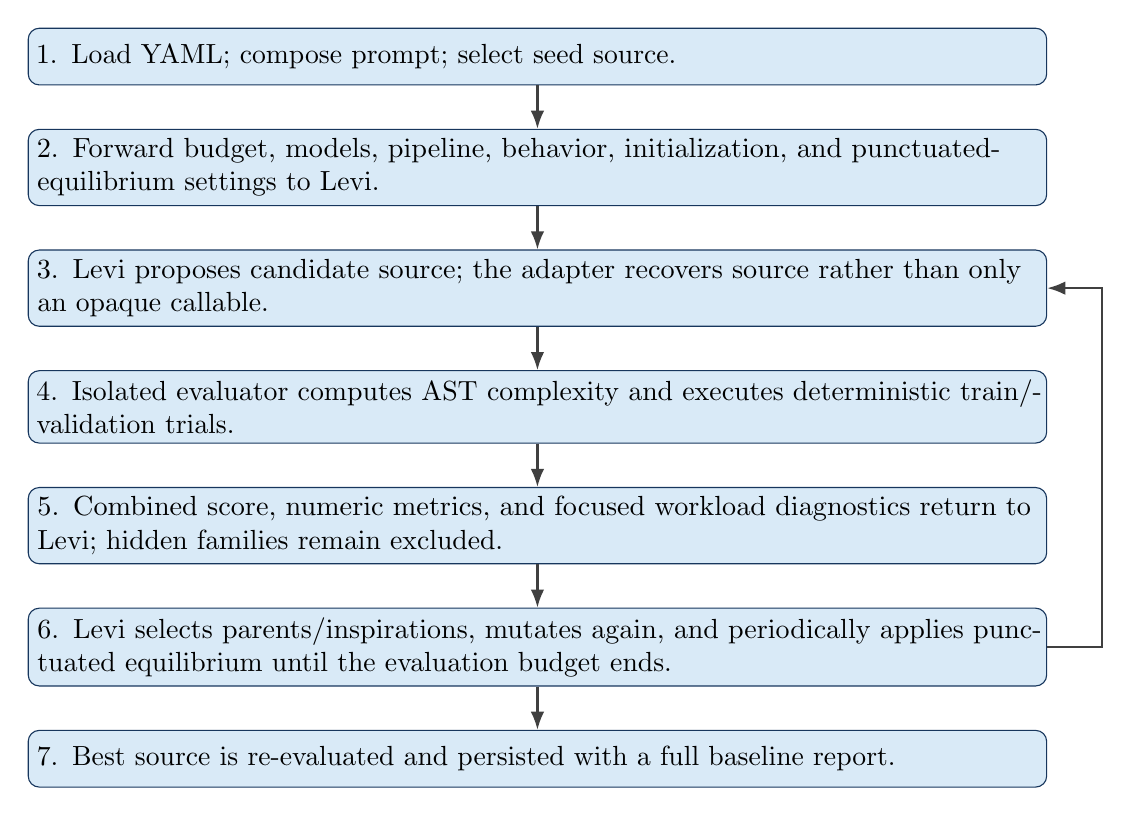
\begin{tikzpicture}[
  node distance=0.55cm,
  box/.style={draw=navy, rounded corners, fill=lightblue, align=left,
              text width=12.7cm, minimum height=0.72cm},
  arrow/.style={-{Latex[length=2.3mm]}, thick, draw=darkgray}
]
  \node[box] (one) {1. Load YAML; compose prompt; select seed source.};
  \node[box, below=of one] (two) {2. Forward budget, models, pipeline, behavior,
  initialization, and punctuated-equilibrium settings to Levi.};
  \node[box, below=of two] (three) {3. Levi proposes candidate source; the adapter
  recovers source rather than only an opaque callable.};
  \node[box, below=of three] (four) {4. Isolated evaluator computes AST complexity and
  executes deterministic train/validation trials.};
  \node[box, below=of four] (five) {5. Combined score, numeric metrics, and focused
  workload diagnostics return to Levi; hidden families remain excluded.};
  \node[box, below=of five] (six) {6. Levi selects parents/inspirations, mutates again,
  and periodically applies punctuated equilibrium until the evaluation budget ends.};
  \node[box, below=of six] (seven) {7. Best source is re-evaluated and persisted with a
  full baseline report.};
  \draw[arrow] (one) -- (two);
  \draw[arrow] (two) -- (three);
  \draw[arrow] (three) -- (four);
  \draw[arrow] (four) -- (five);
  \draw[arrow] (five) -- (six);
  \draw[arrow] (six.east) -- ++(0.7,0) |- (three.east);
  \draw[arrow] (six) -- (seven);
\end{tikzpicture}
\caption{Repository-controlled evolution loop around Levi.}
\label{fig:evolution}
\end{figure}

\subsection{Current search configuration}

\begin{center}
\begin{tabularx}{\textwidth}{>{\ttfamily}p{0.30\textwidth} X}
\toprule
\normalfont\textbf{Setting} & \textbf{Current value and effect} \\
\midrule
max\_iterations & YAML default 300; CLI \code{--iterations} overrides it and is
forwarded as Levi's \code{budget_evals}. \\
mutation\_model & \code{openai/gpt-5.4-mini}, selected from the primary model. \\
paradigm\_model & \code{openai/gpt-5.5}, selected from the secondary model and
reserved for paradigm shifts. \\
sampler-model pairs & Four \code{gpt-5.4-mini} sampling configurations used by the
pipeline. \\
mutation max\_tokens & 6,000, forwarded through the normal mutation pipeline. \\
paradigm max\_tokens & 12,000 for punctuated-equilibrium reasoning calls. \\
n\_llm\_workers & 4. \\
n\_eval\_processes & 2, derived from \code{parallel_evaluations}. \\
eval\_timeout & 90 seconds for isolated candidate evaluation. \\
n\_parents, n\_inspirations & One parent and zero inspirations per normal mutation. \\
init & Four diverse seeds and three variants per retained seed; diverse-seed calls use
medium reasoning effort. \\
cvt & Twelve data-driven centroids, with a fallback when initialization behaviors
collapse to duplicate centroids. \\
punctuated\_equilibrium & Enabled with medium reasoning effort for
\code{gpt-5.5} paradigm-shift calls. \\
behavior & CVT descriptors include cyclomatic complexity, subscript count, validation
cache-economics metrics including avoidable eviction and short reuse after eviction,
agentic-surrogate hit and underfill, and stochastic-mix hit rate. \\
mutation feedback & Every retained parent exposes the agentic surrogate,
stochastic-serving target, and up to three additional weak-workload diagnostics to
normal mutation workers. \\
candidate guardrails & The general lane rejects candidates above 650 effective AST
nodes.  The function-only eviction-specialist lane evaluates ranking functions up to
1000 nodes and requires the final composed deployable policy to remain at most 650.
Rejected source patterns still fail before simulation. \\
\bottomrule
\end{tabularx}
\end{center}

\subsection{Completed mutation-operator productivity}
\label{sec:operator-productivity}

The completed 500-budget function-only eviction-specialist run provides an unusually
clear diagnostic of Levi's punctuated-equilibrium design.  The final snapshot of run
\identifier{20260608_150431_280387} records 498 evaluations, four evaluation errors,
twenty scored seed or initialization entries, and 474 scored post-initialization
proposals.  Table~\ref{tab:operator-productivity} classifies those proposals by their
recorded sampler.  Acceptance means that a proposal entered or replaced a behavior-
archive cell; it does not mean that the proposal became the scalar incumbent.

\begin{table}[H]
\centering
\small
\begin{tabular}{lrrrrr}
\toprule
\textbf{Operator} & \textbf{Scored} & \textbf{Accepted} &
\textbf{Accept rate} & \textbf{New best} & \textbf{New-best rate} \\
\midrule
Normal GPT-5.4-mini mutation & 422 & 74 & \(17.5\%\) & 7 & \(1.7\%\) \\
GPT-5.4-mini PE variant & 39 & 4 & \(10.3\%\) & 3 & \(7.7\%\) \\
Direct GPT-5.5 paradigm shift & 13 & 5 & \(38.5\%\) & 3 & \(23.1\%\) \\
\bottomrule
\end{tabular}
\caption{Operator productivity in the completed eviction-specialist run.
``New best'' means a strict improvement in best score so far.}
\label{tab:operator-productivity}
\end{table}

Combining direct paradigm shifts and their variants, punctuated-equilibrium proposals
were about \(6.9\times\) more likely than normal mutations to establish a new global
best: \(6/52=11.5\%\), versus \(7/422=1.7\%\).  Direct GPT-5.5 paradigm shifts alone
established a new best in three of thirteen attempts.  The final \(72.091\) winner
came from a later normal mutation at evaluation 349, so punctuated equilibrium opened
productive structural neighborhoods without replacing the need for local refinement.

The complementary result is equally important.  From the strongest initialization
score of \(71.075\) to the final best of \(72.091\), normal mutations contributed
\(0.900\), or \(88.6\%\), of the \(1.016\)-point cumulative best-score gain.  The
largest single jump, \(+0.550\), was also a normal mutation.  Most individual normal
mutations therefore fail, but it would be incorrect to conclude that only paradigm
shifts matter.  In this run, paradigm shifts are high-yield structural exploration;
normal mutations provide the dense exploitation and occasional large refinement that
turns those neighborhoods into cumulative progress.  Archive acceptance also preserves
behaviorally distinct stepping stones that a global-best-only count does not credit.

These figures are a single-run diagnostic, not a general operator benchmark.
Independent replicated runs are required to estimate stable operator productivity and
to separate operator effects from model, prompt, parent, and search-stage effects.

\subsection{Prompt engineering as an implementation constraint}

The system prompt documents the exact hook contract and candidate-visible schema.  It
explicitly warns candidates:

\begin{itemize}
  \item only \code{on_request_start}, \code{on_cache_hit}, and \code{on_cache_miss}
  fire as lifecycle callbacks;
  \item \code{id(block)} and guessed attributes are invalid state keys;
  \item future-reuse fields are unavailable to deployable candidates;
  \item recurrence, gap-moment, subtree, and regime context fields are online-only;
  \item canonical bounded multi-timescale primitives are available but optional;
  \item the compact \code{threshold_excess} positive-hinge primitive is optional;
  \item priority is useful QoS metadata but not proof of reuse;
  \item request-tail service, worst-quarter service, wasted admissions, avoidable
  evictions, churn, policy-caused underfill, and complexity affect ranking;
  \item workload-family names and request-type values must not be hard-coded;
  \item the structure probe and hidden workloads must not be inspected for candidate
  selection.
\end{itemize}

This contract is important because earlier evolved candidates repeatedly created inert
\code{on_block_*} or \code{on_request_end} machinery.  Under an unbounded complexity
penalty, unsupported hooks are not only ineffective but directly harmful.
Static and runtime contract failures now emit violation-specific repair instructions,
and mutation prompts include a preflight checklist covering syntax, entry points,
documented fields and callbacks, imports, and complexity headroom.  This keeps Python
as the structural search language while making invalid proposals cheaper to repair.
For valid retained parents, the evaluator emits at most five workload diagnostics:
the non-quarantined \identifier{agentic_tool_workflows} and
\identifier{stochastic_serving_mix} targets are reserved, and the remaining slots go
to the weakest validation workloads.  Levi samples up to three of those diagnostics
into each normal mutation prompt.  Initialization and paradigm-shift prompts still use
their separate prompt builders and do not yet receive this parent-specific feedback.

\subsection{Run chronology}

The following run scores were produced under the verifier version active at the time.
They are useful for search chronology but are \risk{not directly comparable} to the
compact seed's \(74.321\) score under the discovery verifier because the capacity sweep,
workload panel, and score terms were subsequently strengthened.

\begin{center}
\scriptsize
\begin{tabularx}{\textwidth}{@{}lrrrrrX@{}}
\toprule
\textbf{Run ID} & \textbf{Evals} & \textbf{Score} & \textbf{Runtime} &
\textbf{Cost} & \textbf{Archive} & \textbf{Interpretation} \\
\midrule
20260605T075913Z & 100 & 27.052 & 1454.4 s & \$2.173 & 50 &
Budget was consumed by broad initialization; little useful iterative evolution. \\
20260605T081118Z & 98 & 32.128 & 500.7 s & \$0.710 & 1 &
Corrected iterative run from the compact seed; found a stronger but complex policy. \\
manual simplification & -- & 35.927 & -- & -- & -- &
Removed inert/future-reuse/defensive branches while preserving behavior; complexity
dropped from 808 to 422 AST nodes. \\
20260605T082345Z & 98 & 35.927 & 535.7 s & \$0.692 & 1 &
No generated mutation beat the simplified incumbent. \\
coefficient sweep & 180 samples & 38.703 old-verifier final & -- & -- & -- &
Fully evaluated the top 12 sampled compact parameter sets; final source complexity
became 367 nodes. \\
20260606T000036Z & 98 & 57.788 & 1083.2 s & \$2.898 & 8 &
Expanded recurrence/regime observables and primitives; no mutation beat the compact
seed. \\
\bottomrule
\end{tabularx}
\end{center}

The first run exposed a workflow issue: a nominal 100-evaluation budget could be
exhausted in initialization.  Subsequent compact-family runs used zero diverse seeds
and eight variants to preserve most of their budget for iterative mutation.  After
later runs showed collapsed archive diversity and inactive punctuated equilibrium, the
live configuration deliberately reintroduced four diverse seeds, three variants per
retained seed, and twelve data-driven archive centroids.  Complexity changed from a
saturating cap to the current unbounded concave form and later gained the bounded
canonical-primitive subsidy.  The expansion run had that subsidy enabled, but its
strongest valid generated mutation did not use a canonical primitive and therefore
received no discount; Section~\ref{sec:post-expansion} separates that search-adoption
caveat from the policy-quality result.

\subsection{Coefficient sweep}

The reproducible tuner represents the compact policy with 15 parameters covering hit
observation weight, admission frequency/priority/structure/cost/threshold terms, and
eviction age/frequency/structure/priority terms, plus frequency and priority half-lives.
It samples a deterministic discrete grid, ranks candidates on a smaller panel, and
fully evaluates the strongest candidates.  The script defaults to 160 samples and 12
finalists; the recorded final tuning run used 180 samples and 12 finalists.  A separate
\code{--decay-ablation} mode evaluates the four combinations of enabled and disabled
frequency and priority decay on the full panel.

This hybrid process is deliberate:

\begin{itemize}
  \item LLM evolution searches policy structure and can invent state or formulas.
  \item Manual ablation removes behaviorally inert complexity.
  \item Deterministic coefficient search efficiently tunes a compact fixed structure.
\end{itemize}

\section{Compact Policy Family}

\subsection{State}

The compact policy maintains only:

\begin{itemize}
  \item a per-prefix timestamped observed frequency \(f_b\);
  \item a per-prefix timestamped maximum observed request priority \(p_b\);
  \item the current request priority.
\end{itemize}

Frequency and priority share one timestamp because both values are read and refreshed
together.  If \(\Delta t\) logical arrival steps have elapsed since the state was read,
the lazy decay operation is:

\begin{equation}
  D_h(x,\Delta t) = x\,2^{-\Delta t/h}.
\end{equation}

The selected frequency half-life is 12 steps and the selected priority half-life is
1.5 steps.  A miss adds 1.0 to the decayed frequency; a hit adds 2.5.  Priority becomes
the maximum of the decayed prior value and the current request priority.  Setting
either half-life to \code{None} disables only that decay, enabling controlled ablation.
No future information, request-type hard-coding, session map, or unsupported lifecycle
callback is used.

\subsection{Admission equation}

For block \(b\), define:

\begin{equation}
  R_b =
  0.35\log(1+\text{descendants}_b)
  -0.2\max(0,\text{depth}_b-4).
\end{equation}

The admission score is:

\begin{align}
  s_A(b) ={}&
  0.95\log(1+f_b)
  +0.2p_b
  +R_b
  +1.5\log\left(1+\frac{\text{recompute-cost}_b}{96}\right) \nonumber\\
  &-0.7
  -0.24\max(0,\text{depth}_b-2).
\end{align}

The policy therefore requires evidence before admitting most blocks, protects
structurally shared and expensive prefixes, and increasingly resists deep leaves.

\subsection{Eviction equation}

\begin{align}
  s_E(b,t) ={}&
  0.85\log(1+\max(0,t-\text{last-access}_b)) \nonumber\\
  &-1.8\log(1+f_b+\text{hit-count}_b)
  -0.2\log(1+\text{descendants}_b)
  -0.55p_b.
\end{align}

Older blocks become easier to evict, while observed reuse, global hits, structural
fanout, and priority protect a block.

\subsection{Interpretation}

The compact policy's strengths are simple and coherent:

\begin{itemize}
  \item selective admission reduces churn relative to admit-all baselines;
  \item frequency and hit weighting preserve empirically reused prefixes;
  \item recomputation cost and fanout protect valuable trunks;
  \item priority improves burst-recovery service without being the only signal;
  \item logarithms reduce sensitivity to extreme counts and ages.
\end{itemize}

The remaining stale-history term is simulator-owned \(\text{hit-count}_b\), which is
lifetime cumulative and still appears in the eviction equation.  The decayed observed
frequency partly counterbalances it, but a future ablation should test replacing the
lifetime hit count with only recent policy-owned evidence.

\subsection{Promoted pressure-aware extension}

The current incumbent in
\filepath{src/prefix_cache_evolve/problems/prefix_kv_cache/pressure_aware_incumbent.py}
preserves the compact policy's eviction equation and most admission terms.  It adds a
bounded admission-pressure state \(q_t\) derived from the online recent-admission-
pressure and miss-rate signals:

\begin{equation}
  q_t = \min\left(1.5,\;q_{t-1}2^{-1/4}
  + \text{pressure}_t\left(0.75+0.5\min(1,\text{miss-rate}_t)\right)\right).
\end{equation}

Admission subtracts a pressure penalty that increases with depth and decreases with
observed reuse and priority evidence.  The extension also uses last-access-gap evidence
and records priority only on cache hits, avoiding the assumption that a high-priority
miss predicts future reuse.  This policy was promoted only after improving selection,
aggregate probe, both recurrence-heavy probe families, and the hidden panel.
Figures~\ref{fig:incumbent-admission-first}--\ref{fig:incumbent-recurrence-frontier}
separate its admission-first organization, graduated load shedding, and narrow use of
recurrence evidence.

\begin{figure}[H]
\centering
\resizebox{\textwidth}{!}{%
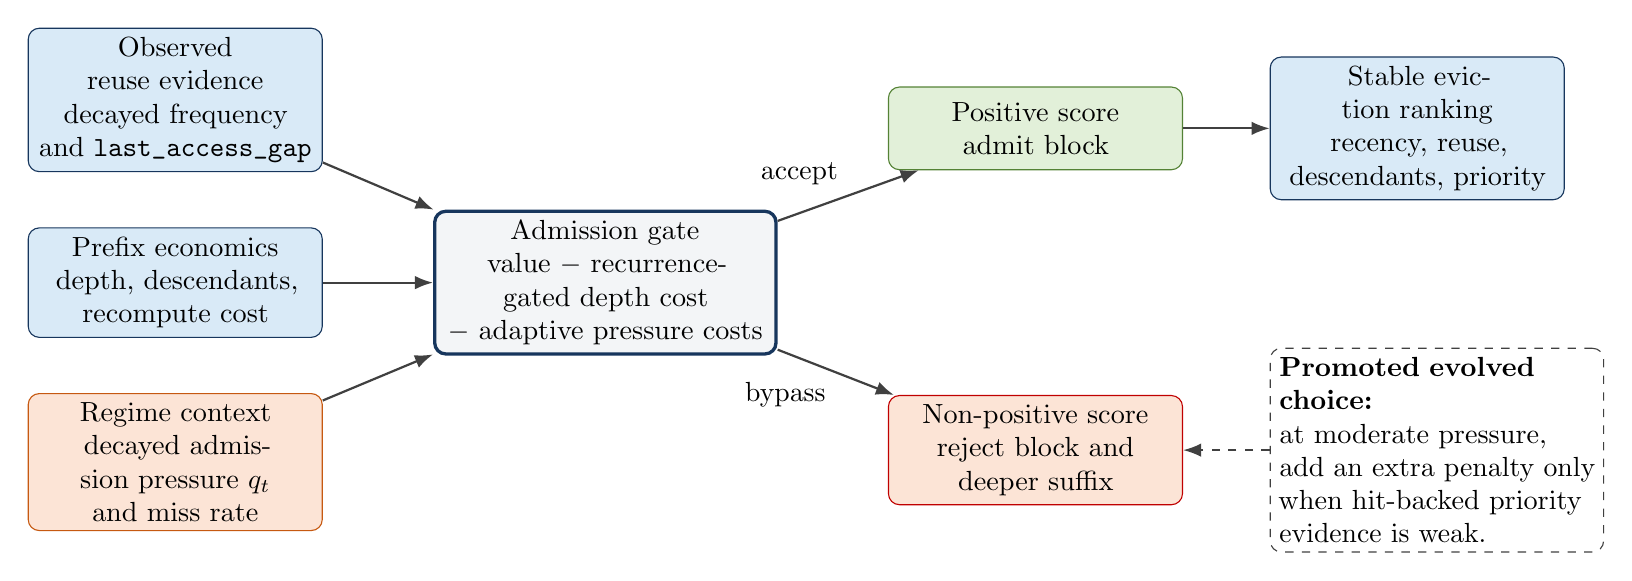
\begin{tikzpicture}[
  node distance=0.7cm and 0.9cm,
  evidence/.style={draw=navy, rounded corners, fill=lightblue, align=center,
                   text width=3.5cm, minimum height=1.05cm},
  regime/.style={draw=orange, rounded corners, fill=lightorange, align=center,
                 text width=3.5cm, minimum height=1.05cm},
  gate/.style={draw=navy, very thick, rounded corners, fill=graybg, align=center,
               text width=4.1cm, minimum height=1.35cm},
  admit/.style={draw=green, rounded corners, fill=lightgreen, align=center,
                text width=3.5cm, minimum height=1.05cm},
  reject/.style={draw=red, rounded corners, fill=lightorange, align=center,
                 text width=3.5cm, minimum height=1.05cm},
  note/.style={draw=darkgray, dashed, rounded corners, fill=white, align=left,
               text width=4.0cm, minimum height=0.9cm},
  arrow/.style={-{Latex[length=2.3mm]}, thick, draw=darkgray}
]
  \node[evidence] (reuse) {Observed reuse evidence\\decayed frequency and
  \code{last_access_gap}};
  \node[evidence, below=of reuse] (economics) {Prefix economics\\depth, descendants,
  recompute cost};
  \node[regime, below=of economics] (regime) {Regime context\\decayed admission pressure
  \(q_t\) and miss rate};

  \node[gate, right=1.4cm of economics] (gate) {Admission gate\\
  value \( - \) recurrence-gated depth cost\\
  \( - \) adaptive pressure costs};
  \node[admit, above right=0.5cm and 1.4cm of gate] (admit) {Positive score\\admit block};
  \node[reject, below right=0.5cm and 1.4cm of gate] (reject) {Non-positive score\\reject
  block and deeper suffix};
  \node[evidence, right=1.1cm of admit] (evict) {Stable eviction ranking\\recency, reuse,
  descendants, priority};
  \node[note, right=1.1cm of reject] (choice) {\textbf{Promoted evolved choice:}\\at
  moderate pressure, add an extra penalty only when hit-backed priority evidence is
  weak.};

  \draw[arrow] (reuse) -- (gate);
  \draw[arrow] (economics) -- (gate);
  \draw[arrow] (regime) -- (gate);
  \draw[arrow] (gate) -- node[above left]{accept} (admit);
  \draw[arrow] (gate) -- node[below left]{bypass} (reject);
  \draw[arrow] (admit) -- (evict);
  \draw[arrow, dashed] (choice) -- (reject);
\end{tikzpicture}
}
\caption{Admission-first organization of the promoted policy.  The evolved mechanisms
primarily prevent low-value blocks from entering the cache; the compact eviction
equation remains unchanged.  Priority is hit-backed evidence, not an unconditional
request-class privilege.}
\label{fig:incumbent-admission-first}
\end{figure}

\begin{figure}[H]
\centering
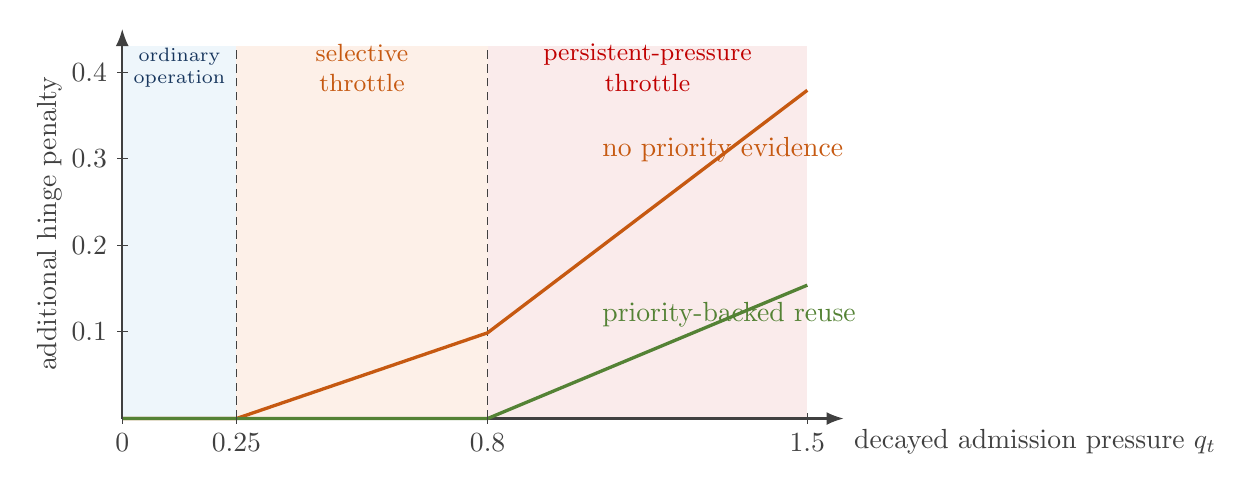
\begin{tikzpicture}[
  x=5.8cm,
  y=11cm,
  axis/.style={-{Latex[length=2.2mm]}, thick, draw=darkgray},
  guide/.style={densely dashed, draw=darkgray},
  low/.style={very thick, draw=orange},
  backed/.style={very thick, draw=green}
]
  \fill[lightblue, opacity=0.45] (0,0) rectangle (0.25,0.43);
  \fill[lightorange, opacity=0.55] (0.25,0) rectangle (0.8,0.43);
  \fill[red, opacity=0.08] (0.8,0) rectangle (1.5,0.43);

  \draw[axis] (0,0) -- (1.58,0)
    node[below right, text=darkgray] {decayed admission pressure \(q_t\)};
  \draw[axis] (0,0) -- (0,0.45);
  \node[rotate=90, anchor=center, text=darkgray] at (-0.16,0.225)
    {additional hinge penalty};
  \draw[guide] (0.25,0) -- (0.25,0.43);
  \draw[guide] (0.8,0) -- (0.8,0.43);

  \draw[low] (0,0) -- (0.25,0) -- (0.8,0.099) -- (1.5,0.379);
  \draw[backed] (0,0) -- (0.8,0) -- (1.5,0.154);

  \foreach \x/\label in {0/0,0.25/0.25,0.8/0.8,1.5/1.5}
    \draw[darkgray] (\x,0.006) -- (\x,-0.006) node[below] {\(\label\)};
  \foreach \y/\label in {0.1/0.1,0.2/0.2,0.3/0.3,0.4/0.4}
    \draw[darkgray] (0.012,\y) -- (-0.012,\y) node[left] {\(\label\)};

  \node[font=\scriptsize, align=center, text=navy] at (0.125,0.405)
    {ordinary\\operation};
  \node[font=\small, align=center, text=orange] at (0.525,0.405)
    {selective\\throttle};
  \node[font=\small, align=center, text=red] at (1.15,0.405)
    {persistent-pressure\\throttle};
  \node[anchor=west, text=orange] at (1.03,0.31) {no priority evidence};
  \node[anchor=west, text=green] at (1.03,0.12) {priority-backed reuse};
\end{tikzpicture}
\caption{The incumbent's graduated pressure response, isolating the two pressure-excess
hinges.  The promoted evolved term starts throttling blocks without priority evidence at
\(q_t=0.25\); the inherited all-block persistent-pressure term starts at \(q_t=0.8\).
The shared depth- and evidence-sensitive pressure penalty is omitted from this
schematic.}
\label{fig:incumbent-pressure-gates}
\end{figure}

\begin{figure}[H]
\centering
\resizebox{0.96\textwidth}{!}{%
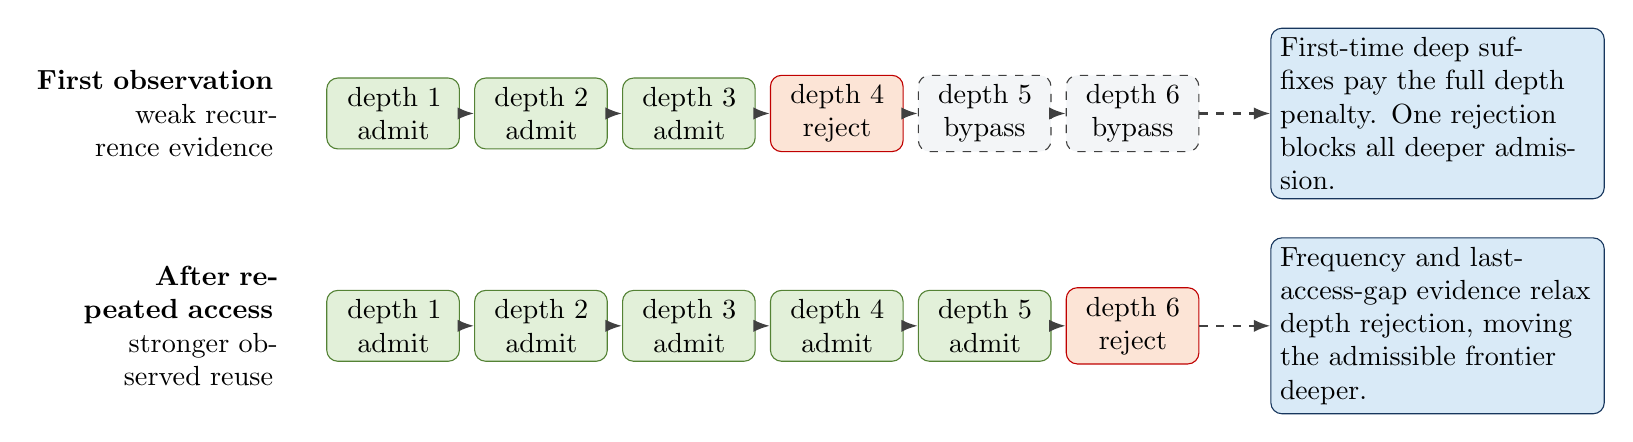
\begin{tikzpicture}[
  node distance=0.18cm,
  admitted/.style={draw=green, rounded corners, fill=lightgreen, align=center,
                   text width=1.45cm, minimum height=0.85cm},
  rejected/.style={draw=red, rounded corners, fill=lightorange, align=center,
                   text width=1.45cm, minimum height=0.85cm},
  bypassed/.style={draw=darkgray, dashed, rounded corners, fill=graybg, align=center,
                   text width=1.45cm, minimum height=0.85cm},
  label/.style={align=right, text width=3.0cm},
  explain/.style={draw=navy, rounded corners, fill=lightblue, align=left,
                  text width=4.0cm, minimum height=1.0cm},
  arrow/.style={-{Latex[length=2.1mm]}, thick, draw=darkgray}
]
  \node[label] (coldlabel) {\textbf{First observation}\\weak recurrence evidence};
  \node[admitted, right=0.55cm of coldlabel] (c1) {depth 1\\admit};
  \node[admitted, right=of c1] (c2) {depth 2\\admit};
  \node[admitted, right=of c2] (c3) {depth 3\\admit};
  \node[rejected, right=of c3] (c4) {depth 4\\reject};
  \node[bypassed, right=of c4] (c5) {depth 5\\bypass};
  \node[bypassed, right=of c5] (c6) {depth 6\\bypass};

  \node[label, below=1.15cm of coldlabel] (repeatlabel) {\textbf{After repeated access}\\
  stronger observed reuse};
  \node[admitted, right=0.55cm of repeatlabel] (r1) {depth 1\\admit};
  \node[admitted, right=of r1] (r2) {depth 2\\admit};
  \node[admitted, right=of r2] (r3) {depth 3\\admit};
  \node[admitted, right=of r3] (r4) {depth 4\\admit};
  \node[admitted, right=of r4] (r5) {depth 5\\admit};
  \node[rejected, right=of r5] (r6) {depth 6\\reject};

  \foreach \a/\b in {c1/c2,c2/c3,c3/c4,c4/c5,c5/c6,r1/r2,r2/r3,r3/r4,r4/r5,r5/r6}
    \draw[arrow] (\a) -- (\b);

  \node[explain, right=0.9cm of c6] (coldnote) {First-time deep suffixes pay the full
  depth penalty.  One rejection blocks all deeper admission.};
  \node[explain, right=0.9cm of r6] (repeatnote) {Frequency and last-access-gap evidence
  relax depth rejection, moving the admissible frontier deeper.};
  \draw[arrow, dashed] (c6) -- (coldnote);
  \draw[arrow, dashed] (r6) -- (repeatnote);
\end{tikzpicture}
}
\caption{Recurrence-gated depth relief.  Recurrence is not a separate replacement
controller; it is a narrow exception to the default rule that deep suffixes are costly.
The exact frontier varies with block economics and pressure.}
\label{fig:incumbent-recurrence-frontier}
\end{figure}

\subsection{Decay-term ablation}

The decay half-lives were selected by screening nearby values on a small panel and then
ranking only on the full three-seed validation panel.  The following controlled
ablation uses identical policy code and excludes complexity equally from all variants:

\begin{center}
\small
\begin{tabular}{lrrrrrr}
\toprule
\textbf{Variant} & \textbf{Raw score} & \textbf{Token hit} &
\textbf{Tok. waste} & \textbf{Utility} & \textbf{Avoidable} &
\textbf{Churn/1k} \\
\midrule
No decay & 64.069 & 0.6437 & 0.5244 & 6.484 & 0.1235 & 749.8 \\
Frequency decay only & 58.160 & 0.6364 & 0.4946 & 7.108 & 0.1259 & 725.3 \\
Priority decay only & \textbf{64.839} & 0.6464 & 0.5236 & 6.499 & 0.1167 & 733.7 \\
Both decays & 64.381 & 0.6444 & 0.4913 & 7.143 & \textbf{0.1100} & \textbf{685.5} \\
\bottomrule
\end{tabular}
\end{center}

After quarantining recurrence-heavy families from selection, priority-only decay has
the highest raw validation score.  Its charged selection score is \(58.247\), compared
with \(57.788\) for both decays.  That apparent gain is a selection overfit: the
priority-only probe score falls from \(40.303\) to \(31.787\), and hidden score falls
from \(-18.616\) to \(-19.128\).  It raises probe-family token hit rates but pays for
them with worse admission/churn behavior.  The recommended compact seed therefore
retains both decays.  This inversion demonstrates why the structure probe must be
reviewed alongside the validation scalar.

\section{Retained Discovery Results and Current Robustness}

\subsection{Historical discovery selection and reporting panel}

The table in this subsection uses the retained \(8\)-token discovery verifier.  It
documents the environment that produced the promoted policy; it is not the operative
production-oriented ranking.  Under the current \(16\)-token default, TinyLFU-LRU leads
the incumbent by \(0.791\) combined-score points, as summarized in the workload-model
section and \filepath{docs/results/block_size_robustness.md}.

\begin{center}
\scriptsize
\resizebox{\textwidth}{!}{%
\begin{tabular}{@{}lrrrrrrrrr@{}}
\toprule
\textbf{Policy} & \textbf{Score} & \textbf{Cap. 48} & \textbf{Cap. 96} &
\textbf{Worst qtr.} & \textbf{Tok. waste} & \textbf{Utility} &
\textbf{Avoid.} & \textbf{Underfill} & \textbf{Churn/1k} \\
\midrule
Oracle future reuse & 97.074 & 0.683 & 0.745 & 0.548 & 0.017 & 13.164 & 0.000 & 0.141 & 43.9 \\
Promoted priority-aware pressure incumbent & 77.230 & 0.674 & 0.687 & 0.521 & 0.407 & 8.143 & 0.074 & 0.070 & 92.7 \\
Prior composed incumbent & 76.630 & 0.674 & 0.687 & 0.521 & 0.421 & 7.944 & 0.065 & 0.067 & 148.7 \\
TinyLFU-LRU & 70.362 & 0.618 & 0.690 & 0.457 & 0.357 & 8.062 & 0.108 & 0.112 & 161.1 \\
Future-reuse heuristic & 69.857 & 0.669 & 0.740 & 0.542 & 0.706 & 2.440 & 0.005 & 0.000 & 1197.3 \\
vLLM APC & 60.178 & 0.621 & 0.696 & 0.496 & 0.486 & 7.973 & 0.128 & 0.056 & 807.9 \\
LRU & 51.186 & 0.627 & 0.721 & 0.503 & 0.718 & 2.268 & 0.119 & 0.000 & 1385.0 \\
Depth-prefer-shallow & 50.409 & 0.628 & 0.715 & 0.497 & 0.724 & 2.214 & 0.167 & 0.000 & 1471.5 \\
No cache & -61.304 & 0.000 & 0.000 & 0.000 & 0.000 & 0.000 & 0.000 & 1.000 & 0.0 \\
\bottomrule
\end{tabular}
}
\end{center}

On the discovery verifier, the promoted incumbent is the strongest deployable policy
by \(6.868\) combined-score points over TinyLFU-LRU. Its recurrence-gated depth relief
closes most of the prior agentic gap while its new low-priority pressure term reduces
churn:

\begin{itemize}
  \item \identifier{agentic_tool_workflows} training token hit: \(0.479\) candidate
  versus \(0.478\) vLLM APC and \(0.537\) oracle;
  \item held-out \identifier{agent_trace_branching} token hit: \(0.376\) candidate
  versus \(0.393\) vLLM APC and \(0.402\) oracle;
  \item request p10 hit: \(0.324\) candidate;
  \item worst-quarter hit: \(0.520\) candidate versus \(0.548\) oracle.
\end{itemize}

The incumbent's ranking benefits primarily from stronger pressure-aware churn control.
Recurrence evidence relaxes depth rejection only after observed repeated access, so
first-time deep suffixes still pay the full penalty.  Its new term begins rejecting
low-priority blocks at moderate pressure while allowing priority evidence to suppress
that extra penalty. Its score breakdown is:

\begin{center}
\begin{tabular}{lr}
\toprule
\textbf{Component} & \textbf{Value} \\
\midrule
Mean workload score & \(+75.009\) \\
Minimum-workload contribution & \(+20.341\) \\
Churn cost & \(-1.391\) \\
Underfill cost & \(-0.835\) \\
Fairness cost & \(-7.663\) \\
Complexity cost & \(-8.232\) \\
\midrule
Combined score & \(\mathbf{77.230}\) \\
\bottomrule
\end{tabular}
\end{center}

\subsection{Reasoning decode-KV robustness}
\label{sec:reasoning-kv-robustness}

The shared-capacity robustness panel evaluates all existing policies on
\identifier{concurrent_long_generation}, \identifier{reasoning_burst},
\identifier{reasoning_burst_shifted}, and \identifier{stochastic_serving_mix}.  It
uses the operative 16-token blocks, capacities \((24,48)\), 96 requests per family,
and seeds \((11,23,37)\).  The prefix-only replay is the control; shared mode charges
generated decode KV against the same capacity.  Decode allocation failure is reported
but is not yet a score term, so raw ranking measures prefix-policy quality under
pressure rather than complete serving feasibility.

\begin{center}
\small
\begin{tabular}{lrrrrr}
\toprule
\textbf{Policy} & \textbf{Prefix rank} & \textbf{Shared rank} &
\textbf{Shared raw} & \textbf{Shared hit} & \textbf{Decode failure} \\
\midrule
Oracle future reuse & 1 & 1 & 61.103 & 0.4749 & 77.3\% \\
Pressure-aware incumbent & 3 & 2 & 57.496 & 0.4716 & 77.5\% \\
vLLM APC & 9 & 3 & 57.438 & 0.4668 & 77.5\% \\
Future-reuse heuristic & 2 & 4 & 56.380 & 0.4724 & 78.3\% \\
Prefix fanout & 5 & 5 & 55.862 & 0.4719 & 78.3\% \\
LRU & 10 & 12 & 54.855 & 0.4697 & 78.3\% \\
\bottomrule
\end{tabular}
\end{center}

The incumbent becomes the strongest deployable policy by raw behavior, but only by
\(0.058\) points over vLLM APC.  Its charged score is \(49.264\), below vLLM APC's
\(57.438\), because the framework charges candidate complexity but does not charge
baseline implementations; raw behavior is therefore the meaningful policy comparison
in this panel.  That near-tie is less important than the systems result: average
incumbent decode allocation failure is \(77.5\%\), including \(91.1\%\) on
\identifier{reasoning_burst} and \(98.1\%\) on its shifted variant.  Shared pressure
reduces incumbent token hit from \(0.7145\) to \(0.4716\).  No prefix eviction policy
can reclaim capacity occupied by active decode KV, so the next useful policy surface
must include scheduler actions such as admission control, preemption, swapping, or
separate prefix/decode budgets.  The complete panel is retained in
\filepath{docs/results/reasoning_kv_robustness.md}.

\subsection{Held-out structure-generalization probe}

The recurrence-heavy probe is reported but excluded from selection.  The promoted
priority-aware pressure incumbent's token hit rates are \(0.376\) on
\identifier{agent_trace_branching} and \(0.881\) on
\identifier{cyclic_working_set_pressure}. Recurrence-gated depth relief raises the
first value while the new term lowers agent-trace churn from \(57.3\) to \(55.6\) per
thousand requests.  Aggregate probe score nevertheless slips from \(75.002\) to
\(74.785\) after complexity charging.  Decomposition shows that no behavioral probe
sub-metric causes the decline: raw probe score improves by \(0.047\), mean and
minimum-workload contribution improve, agent churn falls by \(1.7\) per thousand, and
cyclic hit and churn are unchanged.  The entire charged decline is explained by the
\(0.264\) larger complexity cost.  The automatic agentic surrogate-to-probe tripwire
also passes: the token-hit gap is \(0.1025\), below the \(0.12\) threshold.
Stochastic serving mixes remain the clearest weakness.

\subsection{Pressure-aware evolution chronology}
\label{sec:pressure-aware-promotion}

A nominal 300-evaluation search from the compact seed completed 298 recorded
evaluations, cost \$2.781, and filled three archive cells.  The strongest GPT-5.5
paradigm scored \(74.670\); a subsequent compact mutation refined its pressure-aware
admission mechanism and reached \(76.069\). A focused follow-up separated agent-trace
underfill from stochastic-mix noise and added recurrence-gated depth relief, reaching
\(76.480\). A later diversified 300-budget run completed 298 recorded evaluations,
cost \$3.608, and remained in one archive cell. Its best mutation refined the
persistent-pressure coefficient to \(0.22\); composing that term with recurrence-gated
depth relief reached \(76.630\).

\begin{center}
\scriptsize
\resizebox{\textwidth}{!}{%
\begin{tabular}{lrrrrrrrrrrr}
\toprule
\textbf{Policy} & \textbf{Selection} & \textbf{Raw} & \textbf{Mean} &
\textbf{Min} & \textbf{Churn} & \textbf{Underfill} & \textbf{Cx} &
\textbf{Probe} & \textbf{Agent} & \textbf{Cyclic} & \textbf{Hidden} \\
\midrule
Compact seed & 74.321 & 80.914 & 73.991 & 21.293 & 5.925 & 0.781 & 473 &
47.425 & 0.2295 & 0.8272 & -1.951 \\
Original pressure-aware policy & 76.069 & 84.185 & 74.870 & 20.251 & 2.464 & 0.810 & 624 &
54.543 & 0.2476 & 0.8812 & 6.527 \\
Recurrence-aware refinement & 76.480 & 84.241 & 75.066 & 20.244 & 2.615 & 0.791 & 588 &
74.602 & 0.3756 & 0.8812 & 7.266 \\
Prior composed incumbent & 76.630 & 84.598 & 75.044 & 20.251 & 2.230 & 0.804 & 609 &
75.002 & 0.3760 & 0.8812 & 9.691 \\
Promoted priority-aware pressure incumbent & 77.230 & 85.462 & 75.009 & 20.341 & 1.391 & 0.835 & 636 &
74.785 & 0.3761 & 0.8812 & 11.158 \\
\bottomrule
\end{tabular}
}
\end{center}

Unlike prior generated candidates, the composed \(76.630\) incumbent clears final
adjudication: selection, aggregate probe, both recurrence-heavy probe families, and
hidden score all improve. The original policy's main operational gain was a churn-cost
reduction from \(5.925\) to \(2.464\). The recurrence-gated refinement sharply improves
agent traces, and the composed persistent-pressure throttle then lowers churn cost
further to \(2.230\) without giving back that gain.

Run \filepath{artifacts/prefix_kv_cache_runs/20260608T001616Z} then tested the targeted
agentic and stochastic guidance.  Its 298 recorded evaluations cost \$4.558, filled
ten archive cells, accepted 18 candidates, and recorded 237 generation or static-check
errors.  The winning mutation appeared at evaluation 81 and remained best through the
end of the run.  It makes exactly one semantic change to admission:

\begin{equation}
  -0.18 \max(0, 1-\text{priority}_b)\max(0, q_t-0.25).
\end{equation}

This term begins throttling low-priority admissions under moderate persistent pressure,
earlier than the existing all-block threshold at \(q_t=0.8\).  Relative to its
\(76.630\) seed, it raises charged selection by \(0.600\), raises raw-before-complexity
score by \(0.863\), lowers validation churn by \(37.6\%\), lowers token-weighted
admission waste from \(0.421\) to \(0.407\), and raises hidden score by \(1.467\).
Validation token hit changes only from \(0.6697\) to \(0.6691\), agent and cyclic probe
hit are effectively unchanged, and agent-probe churn falls slightly.  The cost is 27
effective complexity nodes.  The resulting \(0.217\) charged aggregate-probe decline
is entirely explained by the \(0.264\) complexity-cost increase: raw probe behavior
improves by \(0.047\).  The fourth-term ablation therefore establishes that the term is
load-bearing, while probe decomposition and the passed tripwire establish that it does
not introduce a quiet held-out behavioral regression.  The exact ablation is retained
in \filepath{docs/results/priority_aware_pressure_ablation.md}; the policy is
promoted as the stable incumbent.

The retained discovery-search configuration makes the two remaining weaknesses visible
to mutation
and archive selection without directly optimizing the held-out probe.  Every
mutation receives a reserved diagnostic for the non-quarantined
\identifier{agentic_tool_workflows} surrogate and for
\identifier{stochastic_serving_mix}.  Agentic hit and underfill plus stochastic-mix hit
are also behavior-archive dimensions, so a specialist can survive as a stepping-stone
parent even before it beats the incumbent's combined score.  This intervention changes
mutation guidance and parent diversity, not the combined selection scalar;
\identifier{agent_trace_branching} remains reporting-only.  The new low-priority
pressure term is evidence that this guidance can produce a compact operational
improvement rather than only a workload-specific hit-rate mutation. Every completed
run also persists a fail-closed tripwire that flags an absolute token-hit-rate gap
greater than \(0.12\) between the surrogate and held-out agentic probe.  This detects
surrogate drift without feeding probe performance back into selection.

The methodological finding is more important than the \(0.600\)-point charged gain.
Earlier seed-locked searches optimized the combined scalar from one archive region and
could not structurally preserve specialist steps for both remaining weaknesses.  The
new search instead supplied held-out-faithful, non-quarantined agentic and stochastic
diagnostics to mutation, and made those specialist behaviors archive dimensions.  It
then discovered one compact pressure term that reduces agentic-tool-workflow churn
from \(142.4\) to \(74.7\) and waste from \(0.104\) to \(0.044\), while also reducing
stochastic-mix churn from \(191.0\) to \(164.9\) and waste from \(0.573\) to \(0.556\).
The held-out probe remained excluded from selection; the tripwire pass is what makes
the result credible as improved search structure rather than probe leakage.

\subsection{Eviction-specialist follow-up}
\label{sec:eviction-specialist}

The promoted incumbent has effective complexity 636, leaving only fourteen nodes below
the original 650-node rejection threshold.  A diagnostic of six retained paradigm
candidates found that all six were rejected solely for effective complexity between
669 and 739; four proposed richer eviction rankings.  Rescoring those four with the
hard limit disabled showed that the cap was suppressing measurable alternatives, but
not hiding a clear winner.  Their raw selection scores ranged from \(85.431\) to
\(85.496\), versus \(85.462\) for the incumbent, and none beat the incumbent after the
smooth complexity charge.  One reduced avoidable eviction from \(0.0736\) to
\(0.0637\), demonstrating useful specialist behavior that the scalar winner alone
would discard.

The follow-up therefore separates exploration from promotion rather than removing
complexity pressure.  Configuration
\filepath{configs/prefix_kv_cache_eviction_specialist.yaml} exposes only
\code{score_eviction(block, now, frequency, priority)}.  The evaluator composes that
function with frozen admission and lifecycle callbacks from the stable pressure-aware
incumbent.  The behavior archive includes validation avoidable eviction and
short-reuse-after-eviction missed-token rate.  The evaluator reports those metrics per
selected workload and ranks candidates by raw behavior before the complexity charge.

Every saved specialist winner is composed back into the complete incumbent and
evaluated as deployable source.  Promotion fails closed unless the composed candidate
is at most 650 effective nodes, strictly improves raw selection behavior, and does not
regress charged selection, validation eviction-regret metrics, aggregate probe, either
probe-family token-hit rate, hidden score, or the agentic surrogate-to-probe tripwire.
This prevents either admission regressions or deletion-only gains from winning the
specialist lane.

The completed 500-budget function-only run validates the exploration side of this
design but not promotion.  It improved raw specialist score from the incumbent
equivalent's \(70.989\) to \(72.091\), filled all sixteen archive cells, and found its
best candidate at evaluation 349.  That function alone has 441 effective nodes and
composes to a \(1{,}011\)-node complete policy, so it already fails the 650-node
deployability gate; broader cross-panel checks cannot make it promotable.

A decision-level follow-up confirms that this gain is real victim-ranking behavior
rather than tie-breaking noise.  Across \(5{,}402\) incumbent eviction decisions,
\(77.5\%\) had multiple legal victims, with 10.64 legal victims on average.  The full
specialist changed the selected victim on \(21.5\%\) of decisions.  It corrected 281
avoidable choices while introducing 150, a net reduction of 131; end-to-end replay
raised raw selection by \(1.101\), reduced validation avoidable-eviction rate from
\(0.1530\) to \(0.1350\), and reduced churn from \(168.1\) to \(164.8\) per thousand
requests.

The decomposition also identifies the main useful design.  Guarded age combined with
descendant protection captures \(98.0\%\) of the full specialist's raw selection gain,
but still composes to 775 nodes.  A single deployable coefficient change---increasing
the incumbent descendant-protection weight from \(0.2\) to \(0.6\)---keeps composed
complexity at 636 and gains \(0.168\) raw selection, but loses \(0.006\) hidden score.
It therefore remains a useful distillation result rather than a promotion candidate.
Full counts, split-level regret, and compact variants are retained in
\filepath{docs/results/eviction_policy_analysis.md}.

\subsection{Post-expansion evolution result}
\label{sec:post-expansion}

Run \filepath{artifacts/prefix_kv_cache_runs/20260606T000036Z} used the expanded
observable surface, canonical multi-timescale primitive, form-aware complexity, and
the quarantined probe under the previous \(24/48\)-block verifier.  A nominal
100-evaluation budget produced 98 recorded evaluations, cost \$2.898, filled eight
archive cells, and retained the compact seed at
\(57.788\).  The strongest generated mutation scored \(50.655\).

That headline alone hides the important decomposition.  The table below compares the
incumbent with the highest-scoring \emph{generated} mutation.  ``Raw before
complexity'' retains the operational churn and fairness charges but adds the
complexity charge back to the selection score.

\begin{center}
\scriptsize
\resizebox{\textwidth}{!}{%
\begin{tabular}{lrrrrrrrr}
\toprule
\textbf{Policy} & \textbf{Mean} & \textbf{Min contribution} &
\textbf{Churn cost} & \textbf{Fairness cost} & \textbf{Raw before cx} &
\textbf{Effective cx} & \textbf{Cx cost} & \textbf{Combined} \\
\midrule
Compact incumbent & 68.642 & 13.685 & 10.283 & 7.663 & 64.381 & 473 & 6.593 & 57.788 \\
Best expanded mutation & 65.346 & 14.300 & 7.754 & 7.663 & 64.229 & 1239 & 13.574 & 50.655 \\
\midrule
Mutation minus incumbent & -3.296 & +0.616 & -2.529 & 0.000 & -0.152 & +766 & +6.982 & -7.134 \\
\bottomrule
\end{tabular}%
}
\end{center}

The ``Min contribution'' column is the same signed
\(0.5\min_{G\in\mathcal{G}}S_G\) floor-guard term used throughout the report.  It is
positive here because each policy's weakest validation workload-capacity group still
has a positive score; the same column becomes negative whenever that weakest group
falls below zero.

The best expanded form was therefore raw-competitive rather than plainly worse on
merit: before complexity it trailed by only \(0.152\) points.  Its lower mean workload
score was almost offset by a better minimum-workload contribution and \(2.529\) points
less churn cost.  Complexity then widened the gap by another \(6.982\) points.  The
correct interpretation is primarily case (a)---a nearly tied raw policy sunk by its
larger implementation---with a small case-(b) raw deficit, not a decisive rejection of
the expanded functional form.

The probe decomposition is more mixed:

\begin{center}
\small
\begin{tabular}{lrrrrr}
\toprule
\textbf{Policy} & \textbf{Raw probe} & \textbf{Charged probe} &
\textbf{Agent-branch hit} & \textbf{Cyclic hit} & \textbf{Churn/1k} \\
\midrule
Compact incumbent & 46.896 & 40.303 & 0.2268 & 0.7817 & 170.1 \\
Best expanded mutation & 38.006 & 24.432 & 0.2574 & 0.7434 & 513.9 \\
\bottomrule
\end{tabular}
\end{center}

The mutation improved the specifically weak
\identifier{agent_trace_branching} family by \(0.0307\) token-hit-rate points, but it
regressed \identifier{cyclic_working_set_pressure} by \(0.0384\), increased probe
churn from \(170.1\) to \(513.9\) per 1000 requests, and lost on both raw and charged
aggregate probe score.  This is not case (c) at the aggregate-probe level, so the
result does not support moving the entire probe into selection.  It does show that the
expanded signals can change the intended behavior; the next useful ablation is to
isolate the agent-branching gain without the cyclic and complexity regressions.

Form-aware complexity was enabled, but the best mutation hand-rolled fast, slow,
priority, and miss-decay state instead of importing the canonical
\code{MultiTimescaleDecay} primitive.  Its raw and effective complexities are both
\(1239\), so it received zero primitive subsidy.  No viable archived elite exercised
the canonical primitive; the only archived primitive user was invalid.  Consequently,
this run does \emph{not} establish that a subsidized structured policy lost on merit.
It establishes that the search found a promising but verbose hand-rolled structure and
failed to adopt the cheaper provided representation.

The saved winner is byte-identical to \code{compact_seed.py}; validation, probe, and
hidden metrics for the recommended seed were therefore exactly unchanged.  At that
stage, the adjudication rule retained the prior seed because no candidate improved
validation while preserving both quarantined panels.  The full decomposition is
persisted in
\filepath{artifacts/prefix_kv_cache_runs/20260606T000036Z/best_generated_mutation_decomposition.json}.

\subsection{Structured ablation and repeated-search adjudication}
\label{sec:structured-search}

The next iteration converted the first expansion run's hand-rolled fast, slow,
priority, and miss-decay dictionaries into a bounded canonical
\code{MultiTimescaleDecay.observe_vector} representation.  Before another evolution
run, a behavior-only full-panel ablation isolated which structural terms were carrying
value.  Complexity is set to zero in this table so the rows compare behavior rather
than source size.

\begin{center}
\scriptsize
\resizebox{\textwidth}{!}{%
\begin{tabular}{lrrrrrrrr}
\toprule
\textbf{Variant} & \textbf{Raw selection} & \textbf{Mean} &
\textbf{Min contribution} & \textbf{Churn cost} & \textbf{Raw probe} &
\textbf{Agent hit} & \textbf{Cyclic hit} & \textbf{Probe churn/1k} \\
\midrule
All structured terms & 62.178 & 65.543 & 13.554 & 9.256 & 35.654 & 0.2626 & 0.7408 & 634.5 \\
Without recurrence & 63.762 & 65.436 & 12.826 & 7.198 & 41.373 & 0.2533 & 0.7445 & 306.4 \\
Without subtree & 59.029 & 63.127 & 11.228 & 6.227 & 37.906 & 0.2558 & 0.7362 & 430.6 \\
Without regime & 61.264 & 67.734 & 14.290 & 13.096 & 27.756 & 0.2662 & 0.7267 & 986.1 \\
Without miss state & 62.287 & 65.668 & 13.546 & 9.265 & 32.501 & 0.2626 & 0.7182 & 678.8 \\
Without priority state & 62.298 & 65.674 & 13.554 & 9.266 & 35.654 & 0.2626 & 0.7408 & 634.5 \\
Without recurrence and priority & 63.819 & 65.380 & 12.815 & 7.073 & 41.373 & 0.2533 & 0.7445 & 306.4 \\
Also without miss state & 63.718 & 65.280 & 12.815 & 7.075 & 41.038 & 0.2534 & 0.7411 & 313.4 \\
\bottomrule
\end{tabular}%
}
\end{center}

The ablation gives a sharper result than the undifferentiated expansion-run loss.
The explicit recurrence terms were harmful, increasing churn without improving either
selection or the aggregate probe.  Priority-decay state was behaviorally inert.
Subtree and regime context carried real value: removing either reduced raw selection,
and removing regime conditioning caused severe probe churn.  Miss-decay state was
near-neutral for validation selection but protected cyclic behavior, so it remained
in the selected structured seed.

Deleting recurrence and priority state produced
\filepath{src/prefix_cache_evolve/problems/prefix_kv_cache/seeds/structured_seed.py}.
It is smaller than the compact incumbent after the canonical subsidy, but it trades
validation and aggregate probe score for better hidden and agent-branching behavior:

\begin{center}
\small
\resizebox{\textwidth}{!}{%
\begin{tabular}{lrrrrrrrr}
\toprule
\textbf{Policy} & \textbf{Combined} & \textbf{Raw before cx} &
\textbf{Effective cx} & \textbf{Subsidy} & \textbf{Probe} &
\textbf{Agent hit} & \textbf{Cyclic hit} & \textbf{Hidden} \\
\midrule
Compact incumbent & 57.788 & 64.381 & 473 & 0 & 40.303 & 0.2268 & 0.7817 & -18.616 \\
Structured seed & 57.426 & 63.819 & 454 & 15 & 34.980 & 0.2533 & 0.7445 & -10.815 \\
\bottomrule
\end{tabular}%
}
\end{center}

The structured seed was then used as the parent for three independent nominal
100-evaluation Levi searches.  Each completed 98 recorded evaluations.  The runner now
persists the strongest generated non-seed mutation and automatically evaluates its
validation, probe, hidden, raw-complexity, effective-complexity, and subsidy
decomposition.  This prevents a retained seed from hiding whether evolution discovered
an interesting but unselected functional form.

\begin{center}
\scriptsize
\resizebox{\textwidth}{!}{%
\begin{tabular}{lrrrrrrrrrr}
\toprule
\textbf{Run ID} & \textbf{Evals} & \textbf{Cost} & \textbf{Generated combined} &
\textbf{Raw before cx} & \textbf{Cx} & \textbf{Subsidy} & \textbf{Probe} &
\textbf{Agent hit} & \textbf{Cyclic hit} & \textbf{Hidden} \\
\midrule
20260606T123835Z & 98 & \$2.474 & 49.326 & 64.433 & 1429 & 15 & 22.871 & 0.1648 & 0.7605 & -16.542 \\
20260606T125829Z & 98 & \$2.722 & 51.219 & 65.470 & 1322 & 15 & 20.854 & 0.2727 & 0.8054 & -16.501 \\
20260606T132003Z & 98 & \$2.486 & 49.702 & 62.938 & 1198 & 0 & 35.312 & 0.2142 & 0.7736 & -15.486 \\
\bottomrule
\end{tabular}%
}
\end{center}

All three searches retained the structured seed as the charged winner, and none
improved charged validation while preserving both quarantined panels.  Run
\filepath{artifacts/prefix_kv_cache_structured_runs/20260606T125829Z} is nevertheless
the strongest functional-form finding.  Its generated mutation improved raw selection
from \(63.819\) to \(65.470\), agent-branching hit from \(0.2533\) to \(0.2727\), and
cyclic hit from \(0.7445\) to \(0.8054\).  It then lost \(14.251\) points to complexity,
regressed aggregate probe score to \(20.854\), and regressed hidden score to
\(-16.501\).  Thus the richer form can improve the recurrence behaviors it targets,
but its current operational behavior and implementation size do not generalize.

The primitive-adoption intervention did work.  All 24 archived elites across the
three searches referenced \code{MultiTimescaleDecay.observe_vector}, whereas no viable
elite in the prior expansion run used the canonical primitive.  The remaining failure
is not discoverability of the supplied representation: generated policies still
expanded to \(1198\)--\(1429\) effective nodes.  The bounded subsidy made canonical
state cheaper but correctly did not make surrounding bespoke control flow free.

The full structure probe remains quarantined from selection.  The per-family hit rates
are useful diagnostics, but Run 2 demonstrates why they should not be promoted without
an operational non-regression constraint: both hit rates improved while aggregate
probe score deteriorated sharply.  At that stage, adjudication kept
\code{compact_seed.py} unchanged and treated the structured seed as a useful alternate
parent.  The ablation and repeated-run verdicts are persisted in
\filepath{artifacts/prefix_kv_cache_structured_ablation.json} and
\filepath{artifacts/prefix_kv_cache_structured_runs/adjudication.json}.

\subsection{Hidden-panel diagnostic}

A post-verifier-revision hidden diagnostic produced:

\begin{center}
\small
\scriptsize
\begin{tabular}{lrrrrrrr}
\toprule
\textbf{Policy} & \textbf{Hidden score} & \textbf{Token hit} &
\textbf{Worst-quarter} & \textbf{Tok. waste} & \textbf{Utility} &
\textbf{Avoidable} & \textbf{Churn/1k} \\
\midrule
Oracle future reuse & 21.517 & 0.4863 & 0.3385 & 0.1151 & 6.566 & 0.0000 & 460.8 \\
TinyLFU-LRU & -7.869 & 0.4176 & 0.2653 & 0.5473 & 3.668 & 0.2768 & 1032.7 \\
Compact candidate & -18.616 & 0.4345 & 0.3044 & 0.6519 & 3.348 & 0.1698 & 1537.4 \\
\bottomrule
\end{tabular}
\end{center}

The candidate retains better hidden hit rate and worst-quarter service than TinyLFU,
but its combined score is worse because it admits too much dead content and churns much
more.  This is precisely the kind of distinction the expanded verifier was intended to
surface.

\section{Evolution-Discovered Principles}
\label{sec:evolution-principles}

The detailed chronology and result tables above contain more information than the
retained winner alone.  This section consolidates that information into a principle
ledger so future search does not repeatedly rediscover the same failures.  A
\important{retained principle} is supported by a baseline comparison, controlled
ablation, repeated search adjudication, or a combination of those sources.  The lists
below are retained within the current synthetic benchmark; statements explicitly
qualified with ``currently'' are \important{working principles} whose broader
generality remains unproven.  An \risk{open hypothesis} remains a proposed experiment
rather than a conclusion.

Incomplete run snapshots may corroborate an existing pattern, but they do not establish
new retained principles.  In particular, the June 7 discovery-verifier 30-evaluation
snapshot at \filepath{runs/20260607_151718_996826/snapshot.json} contains generated
elites with \(0.674\)--\(0.683\) validation token hit versus the incumbent's \(0.665\),
but only \(48.1\)--\(53.9\) combined score versus \(74.321\).  Those elites have
\(0.655\)--\(0.729\) token-weighted admission waste, \(746.7\)--\(1256.5\) churn per
1000 requests, and \(1544\)--\(1972\) effective complexity.  This supports the
already-retained cache-economics principle below, but the incomplete run is not treated
as a new ranking result.

\subsection{Policy-design principles}

\begin{enumerate}
  \item \textbf{Selective admission is a first-order decision, not a secondary
  optimization.}  Admit-all baselines often achieve competitive hit rates, especially
  at larger capacity, but pay heavily in dead admissions and churn.  The compact
  incumbent and TinyLFU-LRU demonstrate that rejecting low-evidence suffixes can
  outperform indiscriminate retention.  Admission and eviction must therefore be
  designed together; a sophisticated victim score cannot fully repair a polluted
  cache.

  \item \textbf{Shared trunks deserve protection, while deep suffixes require stronger
  evidence.}  The compact incumbent protects fanout and recomputation cost while
  increasingly resisting deep blocks.  The structured ablation independently shows
  that removing subtree context reduces raw selection quality.  Static depth or fanout
  alone is insufficient, as the corresponding single-signal baselines trail the
  incumbent, but structural value is a useful complement to observed reuse.

  \item \textbf{Online regime context improves robustness more than headline mean
  performance.}  Removing recent admission-pressure and miss-rate conditioning raised
  the structured policy's mean workload score, but reduced raw selection, sharply
  increased churn, and damaged the aggregate probe.  Regime signals are therefore most
  valuable as control inputs that prevent unstable behavior during shifts, rather than
  as direct reuse predictors.

  \item \textbf{Explicit access-gap recurrence formulas are not automatically useful
  recurrence models.}  The tested gap-mean and gap-variance terms increased churn and
  hurt both selection and aggregate probe behavior.  Deleting them was beneficial.
  Recurrence should be represented only when it survives ablation; bounded
  multi-timescale observations are a safer search substrate than assuming that a
  hand-written gap formula is predictive.

  \item \textbf{Miss evidence is a guardrail, not a dominant value signal.}  Removing
  miss-decay state was nearly neutral on validation selection but materially weakened
  cyclic behavior.  This supports retaining a compact miss-pressure channel when it
  prevents repeated pollution or cycling failures, while rejecting large miss-state
  subsystems that do not earn their complexity.

  \item \textbf{Priority is a QoS modifier, not proof of future reuse.}  The incumbent
  uses priority only alongside frequency, structure, depth, and recomputation cost.
  The structured priority-decay channel was behaviorally inert, and the
  \identifier{priority_one_off_noise} families show why long-lived protection based
  only on priority is unsafe.  Policies should protect recurring priority traffic
  without allowing high-priority one-offs to displace reusable normal traffic.

  \item \textbf{Decay choices must be adjudicated outside the optimized split.}  In the
  compact decay ablation, priority-only decay won the validation scalar, but both-decay
  state performed better on the quarantined probe and hidden panel and reduced waste,
  avoidable eviction, and churn.  The retained lesson is not that every signal must
  decay identically; it is that stale evidence must be controlled and decay variants
  must be selected for cross-panel robustness rather than a small validation gain.

  \item \textbf{Higher hit rate can be purchased with poor cache economics.}  The
  hidden-panel compact candidate beats TinyLFU-LRU on token hit and worst-quarter hit
  yet loses badly on combined score because it admits more dead content and churns
  more.  Generated mutations repeatedly exhibit the same pattern.  A deployable policy
  must convert admitted capacity into realized saved tokens, not merely increase the
  number of matched blocks.

  \item \textbf{Richer functional form is useful only when its targeted gain survives
  operational and implementation costs.}  Generated structured mutations improved
  agent-branching behavior, and one improved raw validation plus both probe-family hit
  rates.  None survived aggregate probe, hidden, churn, waste, and complexity
  adjudication.  These are real behavioral discoveries, but they are alternate parents
  for simplification rather than deployable winners.

  \item \textbf{Compact composite scores currently generalize better than isolated
  single-signal rules.}  LRU, LFU, recomputation-only, depth-only, fanout-only, and
  fairness-biased baselines each capture a plausible principle but trail the compact
  incumbent.  The current evidence favors small formulas that combine recent reuse,
  structural value, recomputation cost, depth, and bounded priority influence.
\end{enumerate}

\subsection{Verifier and adjudication principles}

\begin{enumerate}
  \item \textbf{Hit rate is necessary but not sufficient.}  Ranking must also account
  for request tails, worst temporal windows, admission waste and utility, avoidable
  evictions, latency, churn, fairness, underfill, and implementation complexity.
  Otherwise search reliably discovers policies that buy hits through excessive
  turnover or dead retention.

  \item \textbf{Low churn is not intrinsically good.}  The compact policy can report
  very low or zero churn on difficult structure workloads by rejecting most suffixes
  and leaving capacity unused.  Policy-caused underfill is therefore required to
  distinguish valuable selectivity from broad bypass.

  \item \textbf{Realized admission outcomes should be token-weighted.}  Binary useful
  versus wasted counts are interpretable, but they treat partial and full blocks
  equally.  Token-weighted waste and saved tokens per admitted slot better represent
  whether the policy used capacity productively.

  \item \textbf{Robustness terms prevent mean-score shortcuts.}  Worst-workload,
  worst-seed, request-tail, and worst-quarter terms reveal regressions hidden by an
  improved average.  The regime ablation is the clearest example: mean performance
  improved while robust selection and operational behavior deteriorated.

  \item \textbf{Probe and hidden panels must remain quarantined from direct
  optimization.}  The decay ablation and repeated structured searches show that a
  validation winner can regress both panels.  Quarantine preserves their value as
  evidence of generalization rather than turning them into additional training splits.

  \item \textbf{Individual probe-family gains require an aggregate operational
  non-regression check.}  The strongest structured mutation improved both
  recurrence-family hit rates while its aggregate probe score deteriorated sharply.
  Per-family hits are diagnostics, not sufficient acceptance criteria.

  \item \textbf{Raw behavior and charged deployability must be reported separately.}
  Adding the complexity charge back revealed that the first expanded mutation was
  nearly tied on raw merit but decisively worse after implementation cost.  This
  decomposition distinguishes a promising functional form that needs simplification
  from a behaviorally weak idea.

  \item \textbf{Future-knowledge policies are audit instruments and ceilings, not
  deployable competitors.}  The constrained next-use oracle measures remaining
  headroom and avoidable decisions.  The weaker future-reuse heuristic also shows that
  access to future counts does not rescue a policy with poor admission and turnover
  behavior.

  \item \textbf{Multiple capacities expose adaptation failures.}  The compact
  incumbent's token-hit rate is nearly flat between 48 and 96 blocks, while several
  baselines exploit the larger cache.  Capacity sweeps prevent a policy tuned to one
  pressure regime from appearing generally optimal.
\end{enumerate}

\subsection{Evolution and search-process principles}

\begin{enumerate}
  \item \textbf{Start from a strong incumbent and preserve budget for iteration.}  The
  first nominal 100-evaluation run spent its budget on broad initialization.  Reducing
  diverse seeds and initializing from the compact incumbent produced more useful
  iterative search.

  \item \textbf{Separate structure search, deletion ablation, and coefficient tuning.}
  LLM evolution is useful for proposing new state and formulas; controlled ablation
  identifies which terms carry value; deterministic tuning efficiently searches a
  retained compact structure.  Treating these as interchangeable wastes evaluations.

  \item \textbf{Deletion is a productive search operator.}  Manual simplification
  preserved behavior while reducing an evolved policy from 808 to 422 AST nodes.
  Structured ablation then improved behavior by deleting recurrence and inert priority
  state.  New state tables and branches should remain provisional until deletion
  demonstrates that they are necessary.

  \item \textbf{Complexity must be charged from exact candidate source, while safety
  and promotion caps remain separate.}  Opaque callable evaluation cannot distinguish
  a concise formula from a large defensive implementation.  Source-based, concave,
  unbounded complexity correctly breaks raw near-ties and discourages dead machinery.
  A higher exploration cap can expose useful structure, but final promotion should
  retain a stricter deployability limit.

  \item \textbf{The candidate contract is part of the search algorithm.}  Earlier
  candidates invented unsupported lifecycle callbacks, object-identity state, guessed
  schemas, and defensive fallback branches.  Precise prompts, stable-key guidance, and
  structured invalid results reduce this unproductive search space.

  \item \textbf{Canonical primitives require explicit discoverability and incentives.}
  Merely providing \code{MultiTimescaleDecay} did not cause viable elites to use it.
  After the prompt and seed were changed to demonstrate
  \code{observe_vector}, all 24 archived elites across three searches adopted the
  primitive.  Search representations must be easy for the generator to see and copy.

  \item \textbf{Primitive subsidies should be bounded.}  Canonical state should be
  cheaper than hand-rolled equivalents, but surrounding bespoke control flow must
  still pay its full cost.  The retained structured searches confirm that primitive
  adoption alone does not make a 1200--1400-node policy deployable.

  \item \textbf{Add primitives only after repeated successful rediscovery.}
  Separate successful searches independently found thresholded pressure-excess terms,
  justifying the small stateless \code{threshold_excess} helper.  Its one-node credit
  is intentionally smaller than the stateful decay credit, preserving pressure to
  simplify surrounding policy logic.

  \item \textbf{Repeat runs and final adjudication are required before replacing an
  incumbent.}  Three independent searches found interesting but different mutations;
  none improved charged validation while preserving both quarantined panels.  A
  single-run headline is insufficient evidence for promotion.

  \item \textbf{Persist the strongest non-seed mutation even when the seed wins.}  A
  retained incumbent can hide useful functional-form discoveries.  Saving and
  decomposing the strongest generated mutation preserves alternate parents and reveals
  whether failure came from behavior, complexity, or generalization.

  \item \textbf{Treat paradigm shifts and normal mutations as complementary operators.}
  The completed eviction-specialist diagnostic in
  Section~\ref{sec:operator-productivity} finds that punctuated-equilibrium proposals
  are about seven times more likely to establish a new global best, while normal
  mutations still contribute most cumulative best-score gain.  This supports
  alternating sparse structural exploration with dense local exploitation rather than
  replacing either operator from a single-run success-rate comparison.
\end{enumerate}

\subsection{Open hypotheses and unresolved principles}

The following items are deliberately not promoted to retained principles:

\begin{itemize}
  \item \risk{A compact form of the strongest structured mutation may retain its raw
  validation and recurrence-family gains.}  This requires deletion-oriented
  simplification and fresh probe/hidden adjudication.
  \item \risk{A compact eviction specialist may reduce avoidable and short-reuse
  eviction while preserving the full policy.}  The function-only lane isolates
  victim-ranking behavior by construction and has produced a raw specialist gain, but
  its best completed-run function composes to \(1{,}011\) nodes and no specialist has yet
  passed the complete-policy promotion gate.
  \item \risk{Lifetime \code{block.hit_count} may overprotect stale prefixes.}  The
  compact policy partly counterbalances it with decayed policy-owned frequency, but a
  controlled replacement ablation has not been run.
  \item \risk{The structure probe may work better as a lexicographic or non-regression
  constraint than as a reported-only panel.}  Directly optimizing its individual hit
  rates is already known to be unsafe; the appropriate constrained-selection mechanism
  remains untested.
  \item \risk{Capacity-aware or byte-weighted policies may change the preferred
  admission tradeoff.}  The current block-count model exposes poor capacity adaptation
  but cannot establish how byte, layer, transfer, or residency costs should alter the
  policy.
  \item \risk{Trace-calibrated and live metadata may reorder the synthetic findings.}
  The metadata-only calibration and replay path exists, but retained principles still
  require confirmation on held-out production-derived traces.
\end{itemize}

\section{Correctness Properties and Test Strategy}

\subsection{Core invariants}

Functional PyTest coverage asserts, among other properties:

\begin{itemize}
  \item hits are root-contiguous;
  \item rejected roots prevent deeper admission;
  \item missed blocks still invoke miss callbacks after deeper admission becomes
  blocked;
  \item active and interior blocks cannot be evicted;
  \item re-admitted blocks become recently used;
  \item failed lookup probes are charged;
  \item future-reuse metadata advances past the current request and handles same-step
  reuse;
  \item the oracle evicts the furthest next reuse;
  \item LRU tie-breaking and baseline distinctions behave as intended;
  \item binary and token-weighted useful/wasted admissions partition successful
  admission intervals and admitted token mass;
  \item full-block-equivalent admission utility distinguishes full and partial blocks;
  \item avoidable-eviction audits distinguish LRU from the oracle;
  \item hidden families do not affect normal combined score;
  \item structure-probe metrics and invalidity do not affect candidate selection;
  \item recurrence timestamps, bounded gap moments, subtree aggregates, and request
  regime windows are deterministic and online-computable;
  \item multi-timescale primitive state is bounded and deterministic;
  \item the smooth complexity charge is unbounded and concave;
  \item specialist evaluation freezes admission and lifecycle callbacks, ranks raw
  eviction behavior, composes winners into complete policies, and fails final
  promotion closed;
  \item form-aware complexity discounts only canonical primitive composition and leaves
  legacy mode runnable;
  \item vector observations apply distinct finite per-channel additions and reject
  mismatched widths;
  \item the selected structured seed uses bounded canonical state and the structured
  ablation harness preserves its default behavior;
  \item the quick report is labeled smoke-only;
  \item Pydantic rejects unknown workflow and evaluator settings and invalid ranges
  before execution;
  \item YAML family and score configuration matches verifier defaults.
\end{itemize}

\subsection{Current verification status}

Under the operative verifier and workload configuration:

\begin{itemize}
  \item the full standalone repository test suite passes;
  \item \code{ruff check .} passes;
  \item TeX Live compilation succeeds;
  \item \code{git diff --check} is clean;
  \item all 29 supported workload families build;
  \item YAML/default workload and score parity is confirmed;
  \item the historical discovery baseline panel preserves credible ordering: oracle
  first, pressure-aware incumbent second, TinyLFU-LRU third, the reporting heuristic
  fourth, and prefix-anchor and vLLM APC following;
  \item on the operative 16-token default, TinyLFU-LRU leads the incumbent by \(0.791\)
  charged points, while the incumbent retains higher validation token hit and much
  lower churn.
\end{itemize}

\section{Limitations and Recommended Next Steps}

\subsection{Simulator limitations}

\begin{itemize}
  \item \textbf{Block capacity rather than byte capacity.} All blocks consume one unit
  despite possible variation in layer count, dtype, model width, or partial-block
  memory.
  \item \textbf{Proxy latency.} The deterministic formula is useful for ranking but does
  not include kernel scheduling, bandwidth, allocator overhead, or device contention.
  \item \textbf{Synthetic traffic.} Workloads encode plausible failure modes but are not
  calibrated from production trace distributions.
  \item \textbf{Single-cache topology.} There is no routing, replication, cache
  partitioning, host offload, or distributed ownership.
  \item \textbf{Shared-KV mode is a demand stress test, not a scheduler.} It exposes
  infeasible decode demand and prefix displacement, but does not model request
  rejection, preemption, swapping, batch formation, or decode slowdown after an
  allocation failure.
  \item \textbf{Exact prefix reuse only.} There is no semantic reuse, chunk reuse outside
  prefix position, or tokenizer/model-version mismatch.
  \item \textbf{Token rather than byte utility.} Admission utility distinguishes token
  count and repeated hits but does not yet model model-dependent bytes, residency time,
  or transfer cost.
  \item \textbf{Audit horizon.} Avoidable eviction uses full future knowledge for
  verification, which is appropriate for regret measurement but should not be confused
  with an implementable signal.
\end{itemize}

\subsection{Verifier limitations}

\begin{itemize}
  \item Score weights encode design preferences and can still steer search toward the
  cheapest gradient.  They should be sensitivity-tested.
  \item Fairness cost currently uses only the \code{multi_tenant_skew} workload even
  though tenant metrics are reported elsewhere.
  \item Hidden workloads are quarantined from selection, but they remain synthetic and
  visible in repository source to human developers.
  \item The minimum workload term can be dominated by one structurally difficult family;
  score breakdowns must be reviewed alongside the scalar.
  \item Current recovery metrics recognize request types containing the word
  \code{recovery}; this is acceptable as verifier instrumentation but is not a general
  production phase detector.
\end{itemize}

\subsection{Evolution limitations}

\begin{itemize}
  \item The LLM search can invent unsupported or dead state despite prompt guidance.
  Complexity discourages this but does not prevent it.
  \item Fine-grained evaluator diagnostics currently guide normal mutations only.
  Initialization and paradigm shifts do not receive parent-specific diagnostics, and
  the workflow has no bounded global memory of rejected ideas or recurring behavioral
  failures.  The eviction-specialist lane narrows the search problem but does not
  remove this limitation.
  \item A full candidate evaluation is relatively expensive, limiting broad structural
  search.
  \item The coefficient tuner optimizes a fixed compact structure and cannot discover
  qualitatively new state representations.
  \item Three additional 98-evaluation searches from the ablated structured seed did
  not beat the compact seed.  Canonical primitive adoption improved, but
  generated programs still accumulated substantial bespoke control flow.
  \item A later 298-evaluation compact-family search promoted the pressure-aware
  incumbent, which improved selection, probe, and hidden adjudication.
\end{itemize}

\subsection{Recommended next experiments}

\begin{enumerate}
  \item Compact or structurally ablate the strongest mutation from run
  \identifier{20260606T125829Z}.  It is the first generated form to improve raw
  validation and both recurrence-family hit rates, but its \(1322\)-node effective
  implementation and aggregate-probe regression prevent acceptance.
  \item Test an archive dimension or search-time non-regression constraint for
  operational probe score.  Final specialist promotion already enforces aggregate and
  per-family probe non-regression; the unresolved question is whether earlier
  constrained retention improves search without leaking the probe into the optimized
  scalar.
  \item Decompose and simplify the completed function-only winner, then replicate the
  eviction-specialist search to test whether raw gains can survive the 650-node
  composed-policy promotion gate.
  \item Replace block-count capacity with byte- or layer-weighted capacity and add
  byte-weighted admission utility.
  \item Extend the shared prefix/decode capacity panel with scheduler actions and an
  explicit decode-failure or SLO objective.  The current reasoning panel's \(77.5\%\)
  incumbent allocation-failure rate shows that eviction-only optimization is the wrong
  control surface under sustained reasoning bursts.
  \item Calibrate workload mixture, prefix depths, arrival bursts, output lengths, and
  tenant phase durations from anonymized production traces, then replay held-out
  trace-derived metadata.
  \item Add routing, tiering, and host-offload simulators so placement policies can be
  compared with single-cache victim scoring.
  \item Add a bounded global failure store and feed recurring repair and behavioral
  failures to initialization and paradigm-shift prompts, which currently lack the
  parent-specific diagnostics available to normal mutations.
  \item Revisit lifetime \code{block.hit_count}; it remains stale permanent state in the
  compact eviction score even after policy-owned frequency decay.
\end{enumerate}

\section{Reproducibility}

\subsection{Run the full baseline report}

\begin{lstlisting}[style=shell]
.venv/bin/python -m prefix_cache_evolve.problems.prefix_kv_cache.runner \
  --baseline-report \
  --candidate-program \
  src/prefix_cache_evolve/problems/prefix_kv_cache/pressure_aware_incumbent.py
\end{lstlisting}

\subsection{Reproduce the historical discovery result and workload panel}

\begin{lstlisting}[style=shell]
.venv/bin/prefix-cache-evolve \
  --workload-manifest \
  --config configs/prefix_kv_cache_discovery.yaml \
  --workload-manifest-output /tmp/discovery_workload_manifest.json

.venv/bin/prefix-cache-evolve \
  --baseline-report \
  --candidate-program \
  src/prefix_cache_evolve/problems/prefix_kv_cache/pressure_aware_incumbent.py \
  --config configs/prefix_kv_cache_discovery.yaml
\end{lstlisting}

\subsection{Run the quarantined reports}

\begin{lstlisting}[style=shell]
.venv/bin/python -m prefix_cache_evolve.problems.prefix_kv_cache.runner \
  --probe-report \
  --candidate-program \
  src/prefix_cache_evolve/problems/prefix_kv_cache/pressure_aware_incumbent.py

.venv/bin/python -m prefix_cache_evolve.problems.prefix_kv_cache.runner \
  --hidden-report \
  --candidate-program \
  src/prefix_cache_evolve/problems/prefix_kv_cache/pressure_aware_incumbent.py
\end{lstlisting}

\subsection{Run a new evolution from the pressure-aware incumbent}

\begin{lstlisting}[style=shell]
.venv/bin/python -m prefix_cache_evolve.problems.prefix_kv_cache.runner \
  --iterations 300 \
  --config configs/prefix_kv_cache.yaml \
  --seed-program \
  src/prefix_cache_evolve/problems/prefix_kv_cache/pressure_aware_incumbent.py
\end{lstlisting}

\subsection{Run eviction-specialist exploration}

\begin{lstlisting}[style=shell]
.venv/bin/python -m prefix_cache_evolve.problems.prefix_kv_cache.runner \
  --iterations 300 \
  --config configs/prefix_kv_cache_eviction_specialist.yaml \
  --artifact-output artifacts/prefix_kv_cache_eviction_specialist_runs
\end{lstlisting}

\subsection{Run the structured ablation and search parent}

\begin{lstlisting}[style=shell]
.venv/bin/python scripts/ablate_prefix_kv_structured.py

.venv/bin/python -m prefix_cache_evolve.problems.prefix_kv_cache.runner \
  --iterations 100 \
  --config configs/prefix_kv_cache.yaml \
  --seed-program \
  src/prefix_cache_evolve/problems/prefix_kv_cache/seeds/structured_seed.py
\end{lstlisting}

\subsection{Run the deterministic compact-policy tuner}

\begin{lstlisting}[style=shell]
.venv/bin/python scripts/tune_prefix_kv_compact.py \
  --samples 180 \
  --full-top 12 \
  --seed 20260605
\end{lstlisting}

\subsection{Run tests and lint}

\begin{lstlisting}[style=shell]
.venv/bin/pytest -q
.venv/bin/ruff check .
\end{lstlisting}

\subsection{Run eviction decision and distillation analysis}

\begin{lstlisting}[style=shell]
.venv/bin/python -m prefix_cache_evolve.tools.analyze_eviction
\end{lstlisting}

\subsection{Run shared reasoning decode-KV robustness analysis}

\begin{lstlisting}[style=shell]
.venv/bin/python -m prefix_cache_evolve.tools.analyze_reasoning_kv
\end{lstlisting}

\subsection{Artifact layout}

Each saved run directory contains core artifacts and may contain the applicable
run-type-specific artifacts:

\begin{itemize}
  \item \filepath{best_program.py}: best source returned by Levi;
  \item \filepath{metrics.json}: flattened evaluator metrics;
  \item \filepath{artifacts.json}: split, workload, capacity, metadata, and score
  breakdown artifacts;
  \item \filepath{metadata.json}: Levi cost and runtime metadata;
  \item \filepath{run_summary.json}: evaluations, cost, runtime, archive size, and seed;
  \item \filepath{config_snapshot.yaml}: operative search configuration, when the run
  was launched from a config file;
  \item \filepath{workload_manifest.json}: deterministic stream summaries and panel
  fingerprint for the operative report configuration;
  \item \filepath{agentic_surrogate_probe_tripwire.json} and
  \filepath{agentic_surrogate_probe_tripwire.md}: automatic pass/flag comparison of
  agentic surrogate and held-out-probe token hit rate;
  \item \filepath{promotion_adjudication.json} and
  \filepath{promotion_adjudication.md}: fail-closed composed complete-policy
  adjudication for specialist runs;
  \item \filepath{promotion_candidate.py}: complete composed policy evaluated by
  function-only specialist promotion;
  \item \filepath{seed_program.py}: exact source used as the search parent when a
  generated non-seed mutation is retained;
  \item \filepath{best_generated_mutation.py} and
  \filepath{best_generated_mutation_snapshot.json}: strongest archived generated
  non-seed, even when the seed remains the returned winner;
  \item \filepath{best_generated_mutation_decomposition.json} and
  \filepath{best_generated_mutation_decomposition.md}: selection, probe, hidden, and
  complexity comparison between the seed and strongest generated mutation, when one is
  available;
  \item \filepath{paradigm_candidates/}: copied paradigm-shift candidates, when Levi
  retained them;
  \item \filepath{baseline_comparison.md}: full candidate-versus-baseline report, or
  \filepath{baseline_comparison_error.json} if report generation failed.
\end{itemize}

\section{Conclusion}

The implemented system deliberately separates three concerns:

\begin{enumerate}
  \item the \textbf{simulator} enforces realistic prefix-tree and active-reference
  constraints while producing deterministic service and cost metrics;
  \item the \textbf{verifier} converts a broad multi-seed workload panel into an
  interpretable robust score without exposing future information to deployable
  candidates;
  \item the \textbf{evolution workflow} searches executable policy source, charges its
  complexity, and persists reproducible artifacts.
\end{enumerate}

The pressure-aware incumbent demonstrates that a compact deployable policy can remain
competitive after the verifier is tightened.  On the operative 16-token default it
narrowly trails TinyLFU-LRU after complexity charging, while retaining higher
validation token hit and substantially lower churn.
Section~\ref{sec:evolution-principles} consolidates the broader lessons: selective
admission, structural and regime context, robust cross-panel adjudication, realized
cache economics, source-based complexity, deletion-oriented search, and precise
generator-facing contracts all matter. Targeted ablation showed that broad explicit
recurrence terms were harmful and priority-decay state was inert. A later focused
refinement showed that recurrence is useful when it only relaxes an otherwise
categorical depth penalty. Updating the
primitive contract and prompt fixed search adoption: all 24 archived elites from three
new searches used canonical vector-decay state.  One generated mutation improved raw
validation and both recurrence-family hit rates, proving that richer functional form
can address the intended behavior, but complexity and aggregate operational
regressions correctly prevented its selection.  A later compact-family search
discovered a pressure-aware policy that reduced churn and improved selection, probe,
and hidden adjudication. Recurrence-gated depth relief then raised agent-trace hit
rate to near the replacement baselines while retaining low churn. The retained
discovery search
then found a one-line priority-aware pressure term that raises selection and hidden
score while cutting validation churn by \(37.6\%\).  Exact ablation shows the term is
load-bearing, while probe decomposition shows its apparent aggregate regression is
entirely complexity accounting: raw probe behavior improves and the agentic tripwire
passes.  It is now the promoted incumbent.

More broadly, the successful run demonstrates that held-out-faithful surrogate
diagnostics in mutation feedback and specialist archive dimensions can expose and
retain a both-weaknesses fix that seed-locked scalar search could not reach.  The
tripwire preserves the probe discipline that makes this methodological result
credible. Stochastic serving mixes remain the clearest weakness, while the compact and
structured seeds remain useful alternate parents for deletion-oriented search.

\appendix

\section{Engineering Journey: From Prototype to Productive Evolution}
\label{app:engineering-journey}

The final architecture can make the project look more direct than it was.  In
practice, obtaining a useful evolution run required much more than connecting an LLM
to a scalar objective.  The simulator had to become credible enough that improvements
meant something; the evaluator had to be deterministic, isolated, source-aware, and
interpretable; the Levi integration had to preserve enough information to diagnose
failed search; and the generator-facing contract had to be narrowed until most
proposals were executable.  Only after those layers were working did longer evolution
runs begin to produce compact mechanisms that survived cross-panel adjudication.

This appendix records that engineering progression.  It is not a claim that every
intermediate implementation was optimal.  Rather, it documents why each layer was
added, what failure exposed its absence, and how the project moved from ``a run can be
launched'' to ``a run can produce evidence worth trusting.''

\subsection{What ``up and running'' actually required}

There were four distinct thresholds of readiness:

\begin{enumerate}
  \item \textbf{The repository could run locally.}  Baseline, simulator, reporting, and
  test development needed a normal editable development installation.  Evolution was
  deliberately kept separate because Levi is installed from Git rather than as a
  normal project dependency.  This prevented baseline-only and offline work from
  acquiring an unnecessary network dependency, but it also meant an evolution
  environment required an additional explicit installation step.

  \item \textbf{An LLM-backed search could execute.}  The evolution process required a
  configured model provider in addition to Levi.  For the recorded OpenAI-backed run,
  explicit approval was obtained before sending the problem prompt, seed and candidate
  source, and evaluator feedback to OpenAI.  The benchmark itself remained synthetic;
  no hidden production prompt content was required.

  \item \textbf{Candidate scores were technically valid.}  Generated Python had to be
  loaded from source, executed in an isolated worker, checked for time and memory
  limits, and evaluated under a stable candidate-visible schema.  A score from an
  opaque callable was insufficient because the complexity of the exact proposed source
  is part of the objective.

  \item \textbf{Search results were scientifically useful.}  A retained best score was
  not enough.  The system needed exact seed and candidate source, configuration
  snapshots, split and workload metrics, the strongest generated non-seed candidate,
  probe and hidden decompositions, and a final promotion decision.  Without those
  artifacts, an unchanged seed could conceal what evolution had actually discovered.
\end{enumerate}

The practical bootstrap path therefore became:

\begin{lstlisting}[style=shell]
.venv/bin/python -m pip install -e '.[dev]'
uv pip install 'levi @ git+https://github.com/ttanv/levi.git'
.venv/bin/pytest -q
.venv/bin/prefix-cache-evolve --iterations 20
\end{lstlisting}

The short run was useful as an integration smoke test, but never treated as evidence
that a policy improved.  Full ranking decisions required the complete deterministic
panel and retained run artifacts.

\subsection{Building a benchmark before optimizing it}

The first major body of work was not evolution.  It was defining a benchmark whose
score could not be improved by exploiting an unrealistic cache model.  Several
details proved consequential:

\begin{itemize}
  \item Prefix hits had to be root-contiguous, and only inactive resident leaves could
  be eviction victims.  Active decode references, interior nodes, admission rollback,
  and repeated logical arrival steps all affected whether a proposed policy was
  meaningful.
  \item The candidate-visible contract had to separate online-computable fields from
  reporting-only future reuse.  Future knowledge was retained for oracle baselines and
  avoidable-eviction audits, but hidden from deployable candidates.
  \item Hit rate alone produced misleading winners.  The verifier grew to include
  token-weighted admission waste, realized admission utility, policy-caused underfill,
  avoidable eviction, churn, latency, request tails, worst temporal windows, priority
  service, and fairness.
  \item A single capacity and one workload mix were not enough.  The final selection
  panel uses multiple capacities, seeds, and shifted workload families, while probe and
  hidden panels remain quarantined for adjudication.
  \item Credibility baselines and a constrained next-use oracle were needed before an
  evolved result could be interpreted.  They distinguish a genuinely strong compact
  policy from a benchmark that is merely easy to game.
\end{itemize}

This work changed the objective repeatedly.  Historical scores are consequently useful
as a record of search progression, but not all are numerically comparable.  The report
keeps those historical results because the verifier changes are themselves part of
the journey: every new metric or workload was introduced in response to a concrete
shortcut or blind spot.

\subsection{Making Levi a reliable experimental component}

The Levi integration also required several iterations.  The repository eventually
wrapped Levi behind a small adapter rather than allowing it to own the experimental
contract directly.

\begin{center}
\footnotesize
\begin{tabularx}{\textwidth}{@{}>{\raggedright\arraybackslash}p{0.21\textwidth}
  >{\raggedright\arraybackslash}X
  >{\raggedright\arraybackslash}X@{}}
\toprule
\textbf{Integration problem} & \textbf{Why it mattered} &
\textbf{Repository-level response} \\
\midrule
Opaque callable evaluation &
The policy could be simulated, but exact source complexity was unavailable and a large
implementation could appear free. &
Recover candidate source in the Levi score adapter and require source-aware evaluation
for evolution. \\
\addlinespace
Generated code could hang, fail, or grow state without bound &
One bad proposal could consume a worker or make results incomparable. &
Run candidate evaluation in an isolated worker with timeout, memory monitoring,
structured invalid results, and a score below representative valid policies. \\
\addlinespace
Levi's scalar result hid diagnostic evidence &
A seed-retaining run revealed little about the strongest generated idea or why it
lost. &
Persist metrics, artifacts, metadata, configuration, exact seed, strongest generated
non-seed source, and selection/probe/hidden decomposition. \\
\addlinespace
Configuration could drift between search and reports &
A candidate could be evolved under one panel and described under another. &
Load the operative YAML in evaluator workers, snapshot it with the run, and use it for
post-run reports. \\
\addlinespace
Generator failures were undifferentiated &
Syntax errors, unsupported callbacks, guessed fields, and excessive complexity all
looked like generic low scores, so later generations could repeat them. &
Emit structured static and runtime repair feedback and forward it through Levi's
per-example feedback channel. \\
\addlinespace
Learned archive centroids could collapse &
Identical centroids left one archive cell and prevented punctuated equilibrium from
activating. &
Add a degenerate-centroid fallback and make archive behavior dimensions reflect
meaningful specialist tradeoffs. \\
\bottomrule
\end{tabularx}
\end{center}

The most persistent interface problem was that the generator did not initially share
the simulator's exact mental model.  Candidates repeatedly invented
\code{on_request_end} and \code{on_block_evicted}, keyed state by \code{id(block)},
probed guessed fields with \code{getattr}, referenced future-reuse metadata, or added
defensive fallback branches.  None of those proposals improved the deployable policy,
but each consumed generation and evaluation budget.  The response was not only a
stricter prompt.  The evaluator added deterministic source checks, violation-specific
repair instructions, and a compact preflight contract covering imports, callbacks,
stable keys, source size, and candidate-visible fields.

Fine-grained behavioral feedback was a later repair.  Initially, the generator mostly
received a scalar score, so it could not tell whether a candidate lost through
underfill, churn, wasted admissions, a weak workload, or complexity.  The evaluator
now returns score components and focused workload diagnostics, including avoidable
eviction and short reuse after eviction.  Levi forwards those diagnostics to normal
mutation workers.  This remains incomplete: initialization and paradigm-shift prompts
do not receive parent-specific feedback, and there is not yet a bounded global failure
store shared across the whole run.

\subsection{Run diary and turning points}

Table~\ref{tab:journey-runs} records the retained discovery-verifier runs that most
directly changed the system.  The earlier June 6 structured experiments used a prior
verifier and are discussed separately below.

\begin{table}[H]
\centering
\footnotesize
\begin{tabularx}{\textwidth}{@{}>{\raggedright\arraybackslash}p{0.18\textwidth}
  >{\raggedright\arraybackslash}p{0.17\textwidth}
  >{\raggedright\arraybackslash}p{0.15\textwidth}
  >{\raggedright\arraybackslash}X@{}}
\toprule
\textbf{Date, run, and purpose} & \textbf{Execution} & \textbf{Best result} &
\textbf{What it taught us} \\
\midrule
Jun. 7\\\identifier{20260607T054053Z}\\First discovery-verifier 100-run &
98 evaluations; \$4.851; 23.3 minutes; 8 cells &
\(74.321\), seed retained &
Generated policy reached 1675 nodes; preserving generated non-seed decomposition
became essential. \\
\addlinespace
Jun. 7\\\identifier{20260607T110029Z}\\Twenty-iteration smoke run &
18 evaluations; \$0.086; 2.4 minutes; 1 cell &
\(74.321\), seed retained &
End-to-end execution worked, but a short run and one archive cell gave no evidence of
improvement. \\
\addlinespace
Jun. 7\\\identifier{20260607T113545Z}\\Repaired 100-run &
98 evaluations; \$1.027; 14.8 minutes; 5 cells &
\(74.321\), seed retained &
The strongest edit was behaviorally inert; exact complexity and diagnostic feedback
were necessary. \\
\addlinespace
Jun. 7\\\identifier{20260607T123644Z}\\Long compact-family search &
298 evaluations; \$2.781; 39.7 minutes; 3 cells &
\(76.069\), new winner &
First clear full-panel gain: pressure-aware admission sharply reduced churn. \\
\addlinespace
Jun. 7\\\identifier{20260607T135914Z}\\Follow-up from new incumbent &
298 evaluations; \$3.608; 39.0 minutes; 1 cell &
\(76.121\), narrow gain &
Found a useful persistent-pressure term, but archive collapse and narrow behavior
limited the standalone result. \\
\addlinespace
Jun. 8\\\identifier{20260608T001616Z}\\Targeted feedback and archive repair &
298 evaluations; \$4.558; 37.5 minutes; 10 cells &
\(77.230\), promoted &
The winner appeared at evaluation 81; targeted surrogate diagnostics and specialist
dimensions produced the promoted policy. \\
\bottomrule
\end{tabularx}
\caption{Retained discovery-verifier evolution journey.}
\label{tab:journey-runs}
\end{table}

\begin{figure}[H]
\centering
\resizebox{\textwidth}{!}{%
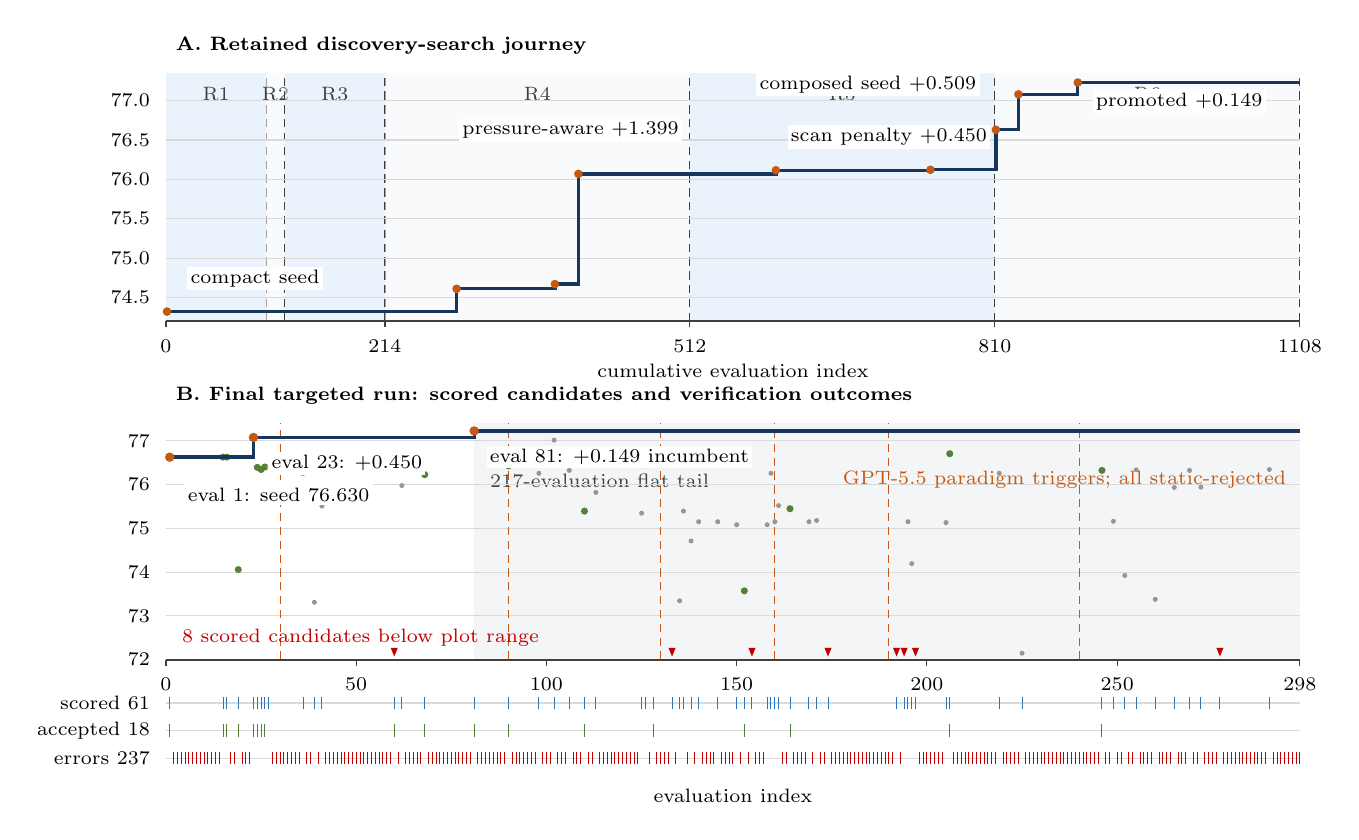
\begin{tikzpicture}[x=1cm,y=1cm]
\node[anchor=west, font=\bfseries\scriptsize] at (1.550,9.700) {A. Retained discovery-search journey};
\fill[lightblue, opacity=0.55] (1.550,6.200) rectangle (2.824,9.350);
\draw[darkgray, densely dashed] (2.824,6.200) -- (2.824,9.350);
\node[font=\scriptsize, anchor=north, text=darkgray] at (2.187,9.300) {R1};
\fill[graybg, opacity=0.55] (2.824,6.200) rectangle (3.058,9.350);
\draw[darkgray, densely dashed] (3.058,6.200) -- (3.058,9.350);
\node[font=\scriptsize, anchor=north, text=darkgray] at (2.941,9.300) {R2};
\fill[lightblue, opacity=0.55] (3.058,6.200) rectangle (4.331,9.350);
\draw[darkgray, densely dashed] (4.331,6.200) -- (4.331,9.350);
\node[font=\scriptsize, anchor=north, text=darkgray] at (3.694,9.300) {R3};
\fill[graybg, opacity=0.55] (4.331,6.200) rectangle (8.204,9.350);
\draw[darkgray, densely dashed] (8.204,6.200) -- (8.204,9.350);
\node[font=\scriptsize, anchor=north, text=darkgray] at (6.268,9.300) {R4};
\fill[lightblue, opacity=0.55] (8.204,6.200) rectangle (12.077,9.350);
\draw[darkgray, densely dashed] (12.077,6.200) -- (12.077,9.350);
\node[font=\scriptsize, anchor=north, text=darkgray] at (10.141,9.300) {R5};
\fill[graybg, opacity=0.55] (12.077,6.200) rectangle (15.950,9.350);
\draw[darkgray, densely dashed] (15.950,6.200) -- (15.950,9.350);
\node[font=\scriptsize, anchor=north, text=darkgray] at (14.014,9.300) {R6};
\draw[darkgray!20] (1.550,6.500) -- (15.950,6.500);
\node[font=\scriptsize, anchor=east] at (1.470,6.500) {74.5};
\draw[darkgray!20] (1.550,7.000) -- (15.950,7.000);
\node[font=\scriptsize, anchor=east] at (1.470,7.000) {75.0};
\draw[darkgray!20] (1.550,7.500) -- (15.950,7.500);
\node[font=\scriptsize, anchor=east] at (1.470,7.500) {75.5};
\draw[darkgray!20] (1.550,8.000) -- (15.950,8.000);
\node[font=\scriptsize, anchor=east] at (1.470,8.000) {76.0};
\draw[darkgray!20] (1.550,8.500) -- (15.950,8.500);
\node[font=\scriptsize, anchor=east] at (1.470,8.500) {76.5};
\draw[darkgray!20] (1.550,9.000) -- (15.950,9.000);
\node[font=\scriptsize, anchor=east] at (1.470,9.000) {77.0};
\draw[very thick, draw=navy] (1.563,6.321) -- (5.241,6.321) -- (5.241,6.610) -- (6.489,6.610) -- (6.489,6.670) -- (6.788,6.670) -- (6.788,8.069) -- (9.296,8.069) -- (9.296,8.115) -- (11.258,8.115) -- (11.258,8.121) -- (12.090,8.121) -- (12.090,8.630) -- (12.376,8.630) -- (12.376,9.080) -- (13.130,9.080) -- (13.130,9.230) -- (15.950,9.230);
\fill[orange] (1.563,6.321) circle (0.055);
\fill[orange] (5.241,6.610) circle (0.055);
\fill[orange] (6.489,6.670) circle (0.055);
\fill[orange] (6.788,8.069) circle (0.055);
\fill[orange] (9.296,8.115) circle (0.055);
\fill[orange] (11.258,8.121) circle (0.055);
\fill[orange] (12.090,8.630) circle (0.055);
\fill[orange] (12.376,9.080) circle (0.055);
\fill[orange] (13.130,9.230) circle (0.055);
\node[font=\scriptsize, anchor=west, fill=white, inner sep=1.2pt] at (1.813,6.741) {compact seed};
\node[font=\scriptsize, anchor=south, fill=white, inner sep=1.2pt] at (6.688,8.469) {pressure-aware +1.399};
\node[font=\scriptsize, anchor=south east, fill=white, inner sep=1.2pt] at (11.890,9.050) {composed seed +0.509};
\node[font=\scriptsize, anchor=north east, fill=white, inner sep=1.2pt] at (12.026,8.700) {scan penalty +0.450};
\node[font=\scriptsize, anchor=north west, fill=white, inner sep=1.2pt] at (13.310,9.150) {promoted +0.149};
\draw[darkgray] (1.550,6.200) -- (1.550,6.120);
\node[font=\scriptsize, anchor=north] at (1.550,6.090) {0};
\draw[darkgray] (4.331,6.200) -- (4.331,6.120);
\node[font=\scriptsize, anchor=north] at (4.331,6.090) {214};
\draw[darkgray] (8.204,6.200) -- (8.204,6.120);
\node[font=\scriptsize, anchor=north] at (8.204,6.090) {512};
\draw[darkgray] (12.077,6.200) -- (12.077,6.120);
\node[font=\scriptsize, anchor=north] at (12.077,6.090) {810};
\draw[darkgray] (15.950,6.200) -- (15.950,6.120);
\node[font=\scriptsize, anchor=north] at (15.950,6.090) {1108};
\draw[darkgray, thick] (1.550,6.200) -- (15.950,6.200);
\node[font=\scriptsize, anchor=north] at (8.750,5.780) {cumulative evaluation index};
\node[anchor=west, font=\bfseries\scriptsize] at (1.550,5.250) {B. Final targeted run: scored candidates and verification outcomes};
\fill[graybg] (5.464,1.900) rectangle (15.950,4.900);
\node[font=\scriptsize, anchor=north west, text=darkgray] at (5.544,4.380) {217-evaluation flat tail};
\draw[darkgray!20] (1.550,1.900) -- (15.950,1.900);
\node[font=\scriptsize, anchor=east] at (1.470,1.900) {72};
\draw[darkgray!20] (1.550,2.456) -- (15.950,2.456);
\node[font=\scriptsize, anchor=east] at (1.470,2.456) {73};
\draw[darkgray!20] (1.550,3.011) -- (15.950,3.011);
\node[font=\scriptsize, anchor=east] at (1.470,3.011) {74};
\draw[darkgray!20] (1.550,3.567) -- (15.950,3.567);
\node[font=\scriptsize, anchor=east] at (1.470,3.567) {75};
\draw[darkgray!20] (1.550,4.122) -- (15.950,4.122);
\node[font=\scriptsize, anchor=east] at (1.470,4.122) {76};
\draw[darkgray!20] (1.550,4.678) -- (15.950,4.678);
\node[font=\scriptsize, anchor=east] at (1.470,4.678) {77};
\draw[orange, densely dashed] (3.000,1.900) -- (3.000,4.900);
\draw[orange, densely dashed] (5.899,1.900) -- (5.899,4.900);
\draw[orange, densely dashed] (7.832,1.900) -- (7.832,4.900);
\draw[orange, densely dashed] (9.282,1.900) -- (9.282,4.900);
\draw[orange, densely dashed] (10.731,1.900) -- (10.731,4.900);
\draw[orange, densely dashed] (13.147,1.900) -- (13.147,4.900);
\node[font=\scriptsize, anchor=north east, text=orange] at (15.900,4.420) {GPT-5.5 paradigm triggers; all static-rejected};
\fill[green] (1.598,4.472) circle (0.045);
\fill[green] (2.275,4.472) circle (0.045);
\fill[green] (2.323,4.472) circle (0.045);
\fill[green] (2.468,3.044) circle (0.045);
\fill[green] (2.661,4.722) circle (0.045);
\fill[green] (2.710,4.342) circle (0.045);
\fill[green] (2.758,4.315) circle (0.045);
\fill[green] (2.806,4.347) circle (0.045);
\fill[darkgray!55] (2.855,4.347) circle (0.032);
\fill[darkgray!55] (3.290,4.264) circle (0.032);
\fill[darkgray!55] (3.435,2.629) circle (0.032);
\fill[darkgray!55] (3.531,3.851) circle (0.032);
\fill[red] (4.449,1.940) -- (4.404,2.050) -- (4.494,2.050) -- cycle;
\fill[darkgray!55] (4.546,4.111) circle (0.032);
\fill[green] (4.836,4.250) circle (0.045);
\fill[green] (5.464,4.805) circle (0.045);
\fill[green] (5.899,4.361) circle (0.045);
\fill[darkgray!55] (6.286,4.267) circle (0.032);
\fill[darkgray!55] (6.479,4.688) circle (0.032);
\fill[darkgray!55] (6.672,4.304) circle (0.032);
\fill[green] (6.865,3.787) circle (0.045);
\fill[darkgray!55] (7.010,4.024) circle (0.032);
\fill[darkgray!55] (7.590,3.760) circle (0.032);
\fill[darkgray!55] (7.639,4.361) circle (0.032);
\fill[green] (7.735,4.516) circle (0.045);
\fill[red] (7.977,1.940) -- (7.932,2.050) -- (8.022,2.050) -- cycle;
\fill[darkgray!55] (8.073,2.648) circle (0.032);
\fill[darkgray!55] (8.122,3.787) circle (0.032);
\fill[darkgray!55] (8.218,3.408) circle (0.032);
\fill[darkgray!55] (8.315,3.652) circle (0.032);
\fill[darkgray!55] (8.557,3.652) circle (0.032);
\fill[darkgray!55] (8.798,3.614) circle (0.032);
\fill[green] (8.895,2.774) circle (0.045);
\fill[red] (8.992,1.940) -- (8.947,2.050) -- (9.037,2.050) -- cycle;
\fill[darkgray!55] (9.185,3.614) circle (0.032);
\fill[darkgray!55] (9.233,4.267) circle (0.032);
\fill[darkgray!55] (9.282,3.652) circle (0.032);
\fill[darkgray!55] (9.330,3.857) circle (0.032);
\fill[green] (9.475,3.817) circle (0.045);
\fill[darkgray!55] (9.716,3.652) circle (0.032);
\fill[darkgray!55] (9.813,3.668) circle (0.032);
\fill[red] (9.958,1.940) -- (9.913,2.050) -- (10.003,2.050) -- cycle;
\fill[red] (10.828,1.940) -- (10.783,2.050) -- (10.873,2.050) -- cycle;
\fill[red] (10.924,1.940) -- (10.879,2.050) -- (10.969,2.050) -- cycle;
\fill[darkgray!55] (10.973,3.652) circle (0.032);
\fill[darkgray!55] (11.021,3.120) circle (0.032);
\fill[red] (11.069,1.940) -- (11.024,2.050) -- (11.114,2.050) -- cycle;
\fill[darkgray!55] (11.456,3.641) circle (0.032);
\fill[green] (11.504,4.516) circle (0.045);
\fill[darkgray!55] (12.133,4.267) circle (0.032);
\fill[darkgray!55] (12.422,1.982) circle (0.032);
\fill[green] (13.437,4.304) circle (0.045);
\fill[darkgray!55] (13.582,3.657) circle (0.032);
\fill[darkgray!55] (13.727,2.969) circle (0.032);
\fill[darkgray!55] (13.872,4.310) circle (0.032);
\fill[darkgray!55] (14.114,2.666) circle (0.032);
\fill[darkgray!55] (14.355,4.087) circle (0.032);
\fill[darkgray!55] (14.549,4.304) circle (0.032);
\fill[darkgray!55] (14.694,4.091) circle (0.032);
\fill[red] (14.935,1.940) -- (14.890,2.050) -- (14.980,2.050) -- cycle;
\fill[darkgray!55] (15.563,4.315) circle (0.032);
\draw[very thick, draw=navy] (1.598,4.472) -- (2.661,4.472) -- (2.661,4.722) -- (5.464,4.722) -- (5.464,4.805) -- (15.950,4.805);
\fill[orange] (1.598,4.472) circle (0.06);
\fill[orange] (2.661,4.722) circle (0.06);
\fill[orange] (5.464,4.805) circle (0.06);
\node[font=\scriptsize, anchor=north west, fill=white, inner sep=1.2pt] at (1.778,4.132) {eval 1: seed 76.630};
\node[font=\scriptsize, anchor=north west, fill=white, inner sep=1.2pt] at (2.841,4.542) {eval 23: +0.450};
\node[font=\scriptsize, anchor=north west, fill=white, inner sep=1.2pt] at (5.614,4.625) {eval 81: +0.149 incumbent};
\node[font=\scriptsize, anchor=south west, text=red] at (1.630,1.950) {8 scored candidates below plot range};
\node[font=\scriptsize, anchor=east] at (1.470,1.350) {scored 61};
\draw[darkgray!20] (1.550,1.350) -- (15.950,1.350);
\draw[blue, line width=0.35pt] (1.598,1.270) -- (1.598,1.430);
\draw[blue, line width=0.35pt] (2.275,1.270) -- (2.275,1.430);
\draw[blue, line width=0.35pt] (2.323,1.270) -- (2.323,1.430);
\draw[blue, line width=0.35pt] (2.468,1.270) -- (2.468,1.430);
\draw[blue, line width=0.35pt] (2.661,1.270) -- (2.661,1.430);
\draw[blue, line width=0.35pt] (2.710,1.270) -- (2.710,1.430);
\draw[blue, line width=0.35pt] (2.758,1.270) -- (2.758,1.430);
\draw[blue, line width=0.35pt] (2.806,1.270) -- (2.806,1.430);
\draw[blue, line width=0.35pt] (2.855,1.270) -- (2.855,1.430);
\draw[blue, line width=0.35pt] (3.290,1.270) -- (3.290,1.430);
\draw[blue, line width=0.35pt] (3.435,1.270) -- (3.435,1.430);
\draw[blue, line width=0.35pt] (3.531,1.270) -- (3.531,1.430);
\draw[blue, line width=0.35pt] (4.449,1.270) -- (4.449,1.430);
\draw[blue, line width=0.35pt] (4.546,1.270) -- (4.546,1.430);
\draw[blue, line width=0.35pt] (4.836,1.270) -- (4.836,1.430);
\draw[blue, line width=0.35pt] (5.464,1.270) -- (5.464,1.430);
\draw[blue, line width=0.35pt] (5.899,1.270) -- (5.899,1.430);
\draw[blue, line width=0.35pt] (6.286,1.270) -- (6.286,1.430);
\draw[blue, line width=0.35pt] (6.479,1.270) -- (6.479,1.430);
\draw[blue, line width=0.35pt] (6.672,1.270) -- (6.672,1.430);
\draw[blue, line width=0.35pt] (6.865,1.270) -- (6.865,1.430);
\draw[blue, line width=0.35pt] (7.010,1.270) -- (7.010,1.430);
\draw[blue, line width=0.35pt] (7.590,1.270) -- (7.590,1.430);
\draw[blue, line width=0.35pt] (7.639,1.270) -- (7.639,1.430);
\draw[blue, line width=0.35pt] (7.735,1.270) -- (7.735,1.430);
\draw[blue, line width=0.35pt] (7.977,1.270) -- (7.977,1.430);
\draw[blue, line width=0.35pt] (8.073,1.270) -- (8.073,1.430);
\draw[blue, line width=0.35pt] (8.122,1.270) -- (8.122,1.430);
\draw[blue, line width=0.35pt] (8.218,1.270) -- (8.218,1.430);
\draw[blue, line width=0.35pt] (8.315,1.270) -- (8.315,1.430);
\draw[blue, line width=0.35pt] (8.557,1.270) -- (8.557,1.430);
\draw[blue, line width=0.35pt] (8.798,1.270) -- (8.798,1.430);
\draw[blue, line width=0.35pt] (8.895,1.270) -- (8.895,1.430);
\draw[blue, line width=0.35pt] (8.992,1.270) -- (8.992,1.430);
\draw[blue, line width=0.35pt] (9.185,1.270) -- (9.185,1.430);
\draw[blue, line width=0.35pt] (9.233,1.270) -- (9.233,1.430);
\draw[blue, line width=0.35pt] (9.282,1.270) -- (9.282,1.430);
\draw[blue, line width=0.35pt] (9.330,1.270) -- (9.330,1.430);
\draw[blue, line width=0.35pt] (9.475,1.270) -- (9.475,1.430);
\draw[blue, line width=0.35pt] (9.716,1.270) -- (9.716,1.430);
\draw[blue, line width=0.35pt] (9.813,1.270) -- (9.813,1.430);
\draw[blue, line width=0.35pt] (9.958,1.270) -- (9.958,1.430);
\draw[blue, line width=0.35pt] (10.828,1.270) -- (10.828,1.430);
\draw[blue, line width=0.35pt] (10.924,1.270) -- (10.924,1.430);
\draw[blue, line width=0.35pt] (10.973,1.270) -- (10.973,1.430);
\draw[blue, line width=0.35pt] (11.021,1.270) -- (11.021,1.430);
\draw[blue, line width=0.35pt] (11.069,1.270) -- (11.069,1.430);
\draw[blue, line width=0.35pt] (11.456,1.270) -- (11.456,1.430);
\draw[blue, line width=0.35pt] (11.504,1.270) -- (11.504,1.430);
\draw[blue, line width=0.35pt] (12.133,1.270) -- (12.133,1.430);
\draw[blue, line width=0.35pt] (12.422,1.270) -- (12.422,1.430);
\draw[blue, line width=0.35pt] (13.437,1.270) -- (13.437,1.430);
\draw[blue, line width=0.35pt] (13.582,1.270) -- (13.582,1.430);
\draw[blue, line width=0.35pt] (13.727,1.270) -- (13.727,1.430);
\draw[blue, line width=0.35pt] (13.872,1.270) -- (13.872,1.430);
\draw[blue, line width=0.35pt] (14.114,1.270) -- (14.114,1.430);
\draw[blue, line width=0.35pt] (14.355,1.270) -- (14.355,1.430);
\draw[blue, line width=0.35pt] (14.549,1.270) -- (14.549,1.430);
\draw[blue, line width=0.35pt] (14.694,1.270) -- (14.694,1.430);
\draw[blue, line width=0.35pt] (14.935,1.270) -- (14.935,1.430);
\draw[blue, line width=0.35pt] (15.563,1.270) -- (15.563,1.430);
\node[font=\scriptsize, anchor=east] at (1.470,1.000) {accepted 18};
\draw[darkgray!20] (1.550,1.000) -- (15.950,1.000);
\draw[green, line width=0.35pt] (1.598,0.920) -- (1.598,1.080);
\draw[green, line width=0.35pt] (2.275,0.920) -- (2.275,1.080);
\draw[green, line width=0.35pt] (2.323,0.920) -- (2.323,1.080);
\draw[green, line width=0.35pt] (2.468,0.920) -- (2.468,1.080);
\draw[green, line width=0.35pt] (2.661,0.920) -- (2.661,1.080);
\draw[green, line width=0.35pt] (2.710,0.920) -- (2.710,1.080);
\draw[green, line width=0.35pt] (2.758,0.920) -- (2.758,1.080);
\draw[green, line width=0.35pt] (2.806,0.920) -- (2.806,1.080);
\draw[green, line width=0.35pt] (4.449,0.920) -- (4.449,1.080);
\draw[green, line width=0.35pt] (4.836,0.920) -- (4.836,1.080);
\draw[green, line width=0.35pt] (5.464,0.920) -- (5.464,1.080);
\draw[green, line width=0.35pt] (5.899,0.920) -- (5.899,1.080);
\draw[green, line width=0.35pt] (6.865,0.920) -- (6.865,1.080);
\draw[green, line width=0.35pt] (7.735,0.920) -- (7.735,1.080);
\draw[green, line width=0.35pt] (8.895,0.920) -- (8.895,1.080);
\draw[green, line width=0.35pt] (9.475,0.920) -- (9.475,1.080);
\draw[green, line width=0.35pt] (11.504,0.920) -- (11.504,1.080);
\draw[green, line width=0.35pt] (13.437,0.920) -- (13.437,1.080);
\node[font=\scriptsize, anchor=east] at (1.470,0.650) {errors 237};
\draw[darkgray!20] (1.550,0.650) -- (15.950,0.650);
\draw[red, line width=0.35pt] (1.647,0.570) -- (1.647,0.730);
\draw[red, line width=0.35pt] (1.695,0.570) -- (1.695,0.730);
\draw[red, line width=0.35pt] (1.743,0.570) -- (1.743,0.730);
\draw[red, line width=0.35pt] (1.792,0.570) -- (1.792,0.730);
\draw[red, line width=0.35pt] (1.840,0.570) -- (1.840,0.730);
\draw[red, line width=0.35pt] (1.888,0.570) -- (1.888,0.730);
\draw[red, line width=0.35pt] (1.937,0.570) -- (1.937,0.730);
\draw[red, line width=0.35pt] (1.985,0.570) -- (1.985,0.730);
\draw[red, line width=0.35pt] (2.033,0.570) -- (2.033,0.730);
\draw[red, line width=0.35pt] (2.082,0.570) -- (2.082,0.730);
\draw[red, line width=0.35pt] (2.130,0.570) -- (2.130,0.730);
\draw[red, line width=0.35pt] (2.178,0.570) -- (2.178,0.730);
\draw[red, line width=0.35pt] (2.227,0.570) -- (2.227,0.730);
\draw[red, line width=0.35pt] (2.371,0.570) -- (2.371,0.730);
\draw[red, line width=0.35pt] (2.420,0.570) -- (2.420,0.730);
\draw[red, line width=0.35pt] (2.516,0.570) -- (2.516,0.730);
\draw[red, line width=0.35pt] (2.565,0.570) -- (2.565,0.730);
\draw[red, line width=0.35pt] (2.613,0.570) -- (2.613,0.730);
\draw[red, line width=0.35pt] (2.903,0.570) -- (2.903,0.730);
\draw[red, line width=0.35pt] (2.951,0.570) -- (2.951,0.730);
\draw[red, line width=0.35pt] (3.000,0.570) -- (3.000,0.730);
\draw[red, line width=0.35pt] (3.048,0.570) -- (3.048,0.730);
\draw[red, line width=0.35pt] (3.096,0.570) -- (3.096,0.730);
\draw[red, line width=0.35pt] (3.145,0.570) -- (3.145,0.730);
\draw[red, line width=0.35pt] (3.193,0.570) -- (3.193,0.730);
\draw[red, line width=0.35pt] (3.241,0.570) -- (3.241,0.730);
\draw[red, line width=0.35pt] (3.338,0.570) -- (3.338,0.730);
\draw[red, line width=0.35pt] (3.386,0.570) -- (3.386,0.730);
\draw[red, line width=0.35pt] (3.483,0.570) -- (3.483,0.730);
\draw[red, line width=0.35pt] (3.580,0.570) -- (3.580,0.730);
\draw[red, line width=0.35pt] (3.628,0.570) -- (3.628,0.730);
\draw[red, line width=0.35pt] (3.676,0.570) -- (3.676,0.730);
\draw[red, line width=0.35pt] (3.724,0.570) -- (3.724,0.730);
\draw[red, line width=0.35pt] (3.773,0.570) -- (3.773,0.730);
\draw[red, line width=0.35pt] (3.821,0.570) -- (3.821,0.730);
\draw[red, line width=0.35pt] (3.869,0.570) -- (3.869,0.730);
\draw[red, line width=0.35pt] (3.918,0.570) -- (3.918,0.730);
\draw[red, line width=0.35pt] (3.966,0.570) -- (3.966,0.730);
\draw[red, line width=0.35pt] (4.014,0.570) -- (4.014,0.730);
\draw[red, line width=0.35pt] (4.063,0.570) -- (4.063,0.730);
\draw[red, line width=0.35pt] (4.111,0.570) -- (4.111,0.730);
\draw[red, line width=0.35pt] (4.159,0.570) -- (4.159,0.730);
\draw[red, line width=0.35pt] (4.208,0.570) -- (4.208,0.730);
\draw[red, line width=0.35pt] (4.256,0.570) -- (4.256,0.730);
\draw[red, line width=0.35pt] (4.304,0.570) -- (4.304,0.730);
\draw[red, line width=0.35pt] (4.353,0.570) -- (4.353,0.730);
\draw[red, line width=0.35pt] (4.401,0.570) -- (4.401,0.730);
\draw[red, line width=0.35pt] (4.498,0.570) -- (4.498,0.730);
\draw[red, line width=0.35pt] (4.594,0.570) -- (4.594,0.730);
\draw[red, line width=0.35pt] (4.643,0.570) -- (4.643,0.730);
\draw[red, line width=0.35pt] (4.691,0.570) -- (4.691,0.730);
\draw[red, line width=0.35pt] (4.739,0.570) -- (4.739,0.730);
\draw[red, line width=0.35pt] (4.788,0.570) -- (4.788,0.730);
\draw[red, line width=0.35pt] (4.884,0.570) -- (4.884,0.730);
\draw[red, line width=0.35pt] (4.933,0.570) -- (4.933,0.730);
\draw[red, line width=0.35pt] (4.981,0.570) -- (4.981,0.730);
\draw[red, line width=0.35pt] (5.029,0.570) -- (5.029,0.730);
\draw[red, line width=0.35pt] (5.078,0.570) -- (5.078,0.730);
\draw[red, line width=0.35pt] (5.126,0.570) -- (5.126,0.730);
\draw[red, line width=0.35pt] (5.174,0.570) -- (5.174,0.730);
\draw[red, line width=0.35pt] (5.222,0.570) -- (5.222,0.730);
\draw[red, line width=0.35pt] (5.271,0.570) -- (5.271,0.730);
\draw[red, line width=0.35pt] (5.319,0.570) -- (5.319,0.730);
\draw[red, line width=0.35pt] (5.367,0.570) -- (5.367,0.730);
\draw[red, line width=0.35pt] (5.416,0.570) -- (5.416,0.730);
\draw[red, line width=0.35pt] (5.512,0.570) -- (5.512,0.730);
\draw[red, line width=0.35pt] (5.561,0.570) -- (5.561,0.730);
\draw[red, line width=0.35pt] (5.609,0.570) -- (5.609,0.730);
\draw[red, line width=0.35pt] (5.657,0.570) -- (5.657,0.730);
\draw[red, line width=0.35pt] (5.706,0.570) -- (5.706,0.730);
\draw[red, line width=0.35pt] (5.754,0.570) -- (5.754,0.730);
\draw[red, line width=0.35pt] (5.802,0.570) -- (5.802,0.730);
\draw[red, line width=0.35pt] (5.851,0.570) -- (5.851,0.730);
\draw[red, line width=0.35pt] (5.947,0.570) -- (5.947,0.730);
\draw[red, line width=0.35pt] (5.996,0.570) -- (5.996,0.730);
\draw[red, line width=0.35pt] (6.044,0.570) -- (6.044,0.730);
\draw[red, line width=0.35pt] (6.092,0.570) -- (6.092,0.730);
\draw[red, line width=0.35pt] (6.141,0.570) -- (6.141,0.730);
\draw[red, line width=0.35pt] (6.189,0.570) -- (6.189,0.730);
\draw[red, line width=0.35pt] (6.237,0.570) -- (6.237,0.730);
\draw[red, line width=0.35pt] (6.334,0.570) -- (6.334,0.730);
\draw[red, line width=0.35pt] (6.382,0.570) -- (6.382,0.730);
\draw[red, line width=0.35pt] (6.431,0.570) -- (6.431,0.730);
\draw[red, line width=0.35pt] (6.527,0.570) -- (6.527,0.730);
\draw[red, line width=0.35pt] (6.576,0.570) -- (6.576,0.730);
\draw[red, line width=0.35pt] (6.624,0.570) -- (6.624,0.730);
\draw[red, line width=0.35pt] (6.720,0.570) -- (6.720,0.730);
\draw[red, line width=0.35pt] (6.769,0.570) -- (6.769,0.730);
\draw[red, line width=0.35pt] (6.817,0.570) -- (6.817,0.730);
\draw[red, line width=0.35pt] (6.914,0.570) -- (6.914,0.730);
\draw[red, line width=0.35pt] (6.962,0.570) -- (6.962,0.730);
\draw[red, line width=0.35pt] (7.059,0.570) -- (7.059,0.730);
\draw[red, line width=0.35pt] (7.107,0.570) -- (7.107,0.730);
\draw[red, line width=0.35pt] (7.155,0.570) -- (7.155,0.730);
\draw[red, line width=0.35pt] (7.204,0.570) -- (7.204,0.730);
\draw[red, line width=0.35pt] (7.252,0.570) -- (7.252,0.730);
\draw[red, line width=0.35pt] (7.300,0.570) -- (7.300,0.730);
\draw[red, line width=0.35pt] (7.349,0.570) -- (7.349,0.730);
\draw[red, line width=0.35pt] (7.397,0.570) -- (7.397,0.730);
\draw[red, line width=0.35pt] (7.445,0.570) -- (7.445,0.730);
\draw[red, line width=0.35pt] (7.494,0.570) -- (7.494,0.730);
\draw[red, line width=0.35pt] (7.542,0.570) -- (7.542,0.730);
\draw[red, line width=0.35pt] (7.687,0.570) -- (7.687,0.730);
\draw[red, line width=0.35pt] (7.784,0.570) -- (7.784,0.730);
\draw[red, line width=0.35pt] (7.832,0.570) -- (7.832,0.730);
\draw[red, line width=0.35pt] (7.880,0.570) -- (7.880,0.730);
\draw[red, line width=0.35pt] (7.929,0.570) -- (7.929,0.730);
\draw[red, line width=0.35pt] (8.025,0.570) -- (8.025,0.730);
\draw[red, line width=0.35pt] (8.170,0.570) -- (8.170,0.730);
\draw[red, line width=0.35pt] (8.267,0.570) -- (8.267,0.730);
\draw[red, line width=0.35pt] (8.363,0.570) -- (8.363,0.730);
\draw[red, line width=0.35pt] (8.412,0.570) -- (8.412,0.730);
\draw[red, line width=0.35pt] (8.460,0.570) -- (8.460,0.730);
\draw[red, line width=0.35pt] (8.508,0.570) -- (8.508,0.730);
\draw[red, line width=0.35pt] (8.605,0.570) -- (8.605,0.730);
\draw[red, line width=0.35pt] (8.653,0.570) -- (8.653,0.730);
\draw[red, line width=0.35pt] (8.702,0.570) -- (8.702,0.730);
\draw[red, line width=0.35pt] (8.750,0.570) -- (8.750,0.730);
\draw[red, line width=0.35pt] (8.847,0.570) -- (8.847,0.730);
\draw[red, line width=0.35pt] (8.943,0.570) -- (8.943,0.730);
\draw[red, line width=0.35pt] (9.040,0.570) -- (9.040,0.730);
\draw[red, line width=0.35pt] (9.088,0.570) -- (9.088,0.730);
\draw[red, line width=0.35pt] (9.137,0.570) -- (9.137,0.730);
\draw[red, line width=0.35pt] (9.378,0.570) -- (9.378,0.730);
\draw[red, line width=0.35pt] (9.427,0.570) -- (9.427,0.730);
\draw[red, line width=0.35pt] (9.523,0.570) -- (9.523,0.730);
\draw[red, line width=0.35pt] (9.571,0.570) -- (9.571,0.730);
\draw[red, line width=0.35pt] (9.620,0.570) -- (9.620,0.730);
\draw[red, line width=0.35pt] (9.668,0.570) -- (9.668,0.730);
\draw[red, line width=0.35pt] (9.765,0.570) -- (9.765,0.730);
\draw[red, line width=0.35pt] (9.861,0.570) -- (9.861,0.730);
\draw[red, line width=0.35pt] (9.910,0.570) -- (9.910,0.730);
\draw[red, line width=0.35pt] (10.006,0.570) -- (10.006,0.730);
\draw[red, line width=0.35pt] (10.055,0.570) -- (10.055,0.730);
\draw[red, line width=0.35pt] (10.103,0.570) -- (10.103,0.730);
\draw[red, line width=0.35pt] (10.151,0.570) -- (10.151,0.730);
\draw[red, line width=0.35pt] (10.200,0.570) -- (10.200,0.730);
\draw[red, line width=0.35pt] (10.248,0.570) -- (10.248,0.730);
\draw[red, line width=0.35pt] (10.296,0.570) -- (10.296,0.730);
\draw[red, line width=0.35pt] (10.345,0.570) -- (10.345,0.730);
\draw[red, line width=0.35pt] (10.393,0.570) -- (10.393,0.730);
\draw[red, line width=0.35pt] (10.441,0.570) -- (10.441,0.730);
\draw[red, line width=0.35pt] (10.490,0.570) -- (10.490,0.730);
\draw[red, line width=0.35pt] (10.538,0.570) -- (10.538,0.730);
\draw[red, line width=0.35pt] (10.586,0.570) -- (10.586,0.730);
\draw[red, line width=0.35pt] (10.635,0.570) -- (10.635,0.730);
\draw[red, line width=0.35pt] (10.683,0.570) -- (10.683,0.730);
\draw[red, line width=0.35pt] (10.731,0.570) -- (10.731,0.730);
\draw[red, line width=0.35pt] (10.780,0.570) -- (10.780,0.730);
\draw[red, line width=0.35pt] (10.876,0.570) -- (10.876,0.730);
\draw[red, line width=0.35pt] (11.118,0.570) -- (11.118,0.730);
\draw[red, line width=0.35pt] (11.166,0.570) -- (11.166,0.730);
\draw[red, line width=0.35pt] (11.214,0.570) -- (11.214,0.730);
\draw[red, line width=0.35pt] (11.263,0.570) -- (11.263,0.730);
\draw[red, line width=0.35pt] (11.311,0.570) -- (11.311,0.730);
\draw[red, line width=0.35pt] (11.359,0.570) -- (11.359,0.730);
\draw[red, line width=0.35pt] (11.408,0.570) -- (11.408,0.730);
\draw[red, line width=0.35pt] (11.553,0.570) -- (11.553,0.730);
\draw[red, line width=0.35pt] (11.601,0.570) -- (11.601,0.730);
\draw[red, line width=0.35pt] (11.649,0.570) -- (11.649,0.730);
\draw[red, line width=0.35pt] (11.698,0.570) -- (11.698,0.730);
\draw[red, line width=0.35pt] (11.746,0.570) -- (11.746,0.730);
\draw[red, line width=0.35pt] (11.794,0.570) -- (11.794,0.730);
\draw[red, line width=0.35pt] (11.843,0.570) -- (11.843,0.730);
\draw[red, line width=0.35pt] (11.891,0.570) -- (11.891,0.730);
\draw[red, line width=0.35pt] (11.939,0.570) -- (11.939,0.730);
\draw[red, line width=0.35pt] (11.988,0.570) -- (11.988,0.730);
\draw[red, line width=0.35pt] (12.036,0.570) -- (12.036,0.730);
\draw[red, line width=0.35pt] (12.084,0.570) -- (12.084,0.730);
\draw[red, line width=0.35pt] (12.181,0.570) -- (12.181,0.730);
\draw[red, line width=0.35pt] (12.229,0.570) -- (12.229,0.730);
\draw[red, line width=0.35pt] (12.278,0.570) -- (12.278,0.730);
\draw[red, line width=0.35pt] (12.326,0.570) -- (12.326,0.730);
\draw[red, line width=0.35pt] (12.374,0.570) -- (12.374,0.730);
\draw[red, line width=0.35pt] (12.471,0.570) -- (12.471,0.730);
\draw[red, line width=0.35pt] (12.519,0.570) -- (12.519,0.730);
\draw[red, line width=0.35pt] (12.567,0.570) -- (12.567,0.730);
\draw[red, line width=0.35pt] (12.616,0.570) -- (12.616,0.730);
\draw[red, line width=0.35pt] (12.664,0.570) -- (12.664,0.730);
\draw[red, line width=0.35pt] (12.712,0.570) -- (12.712,0.730);
\draw[red, line width=0.35pt] (12.761,0.570) -- (12.761,0.730);
\draw[red, line width=0.35pt] (12.809,0.570) -- (12.809,0.730);
\draw[red, line width=0.35pt] (12.857,0.570) -- (12.857,0.730);
\draw[red, line width=0.35pt] (12.906,0.570) -- (12.906,0.730);
\draw[red, line width=0.35pt] (12.954,0.570) -- (12.954,0.730);
\draw[red, line width=0.35pt] (13.002,0.570) -- (13.002,0.730);
\draw[red, line width=0.35pt] (13.051,0.570) -- (13.051,0.730);
\draw[red, line width=0.35pt] (13.099,0.570) -- (13.099,0.730);
\draw[red, line width=0.35pt] (13.147,0.570) -- (13.147,0.730);
\draw[red, line width=0.35pt] (13.196,0.570) -- (13.196,0.730);
\draw[red, line width=0.35pt] (13.244,0.570) -- (13.244,0.730);
\draw[red, line width=0.35pt] (13.292,0.570) -- (13.292,0.730);
\draw[red, line width=0.35pt] (13.341,0.570) -- (13.341,0.730);
\draw[red, line width=0.35pt] (13.389,0.570) -- (13.389,0.730);
\draw[red, line width=0.35pt] (13.486,0.570) -- (13.486,0.730);
\draw[red, line width=0.35pt] (13.534,0.570) -- (13.534,0.730);
\draw[red, line width=0.35pt] (13.631,0.570) -- (13.631,0.730);
\draw[red, line width=0.35pt] (13.679,0.570) -- (13.679,0.730);
\draw[red, line width=0.35pt] (13.776,0.570) -- (13.776,0.730);
\draw[red, line width=0.35pt] (13.824,0.570) -- (13.824,0.730);
\draw[red, line width=0.35pt] (13.920,0.570) -- (13.920,0.730);
\draw[red, line width=0.35pt] (13.969,0.570) -- (13.969,0.730);
\draw[red, line width=0.35pt] (14.017,0.570) -- (14.017,0.730);
\draw[red, line width=0.35pt] (14.065,0.570) -- (14.065,0.730);
\draw[red, line width=0.35pt] (14.162,0.570) -- (14.162,0.730);
\draw[red, line width=0.35pt] (14.210,0.570) -- (14.210,0.730);
\draw[red, line width=0.35pt] (14.259,0.570) -- (14.259,0.730);
\draw[red, line width=0.35pt] (14.307,0.570) -- (14.307,0.730);
\draw[red, line width=0.35pt] (14.404,0.570) -- (14.404,0.730);
\draw[red, line width=0.35pt] (14.452,0.570) -- (14.452,0.730);
\draw[red, line width=0.35pt] (14.500,0.570) -- (14.500,0.730);
\draw[red, line width=0.35pt] (14.597,0.570) -- (14.597,0.730);
\draw[red, line width=0.35pt] (14.645,0.570) -- (14.645,0.730);
\draw[red, line width=0.35pt] (14.742,0.570) -- (14.742,0.730);
\draw[red, line width=0.35pt] (14.790,0.570) -- (14.790,0.730);
\draw[red, line width=0.35pt] (14.839,0.570) -- (14.839,0.730);
\draw[red, line width=0.35pt] (14.887,0.570) -- (14.887,0.730);
\draw[red, line width=0.35pt] (14.984,0.570) -- (14.984,0.730);
\draw[red, line width=0.35pt] (15.032,0.570) -- (15.032,0.730);
\draw[red, line width=0.35pt] (15.080,0.570) -- (15.080,0.730);
\draw[red, line width=0.35pt] (15.129,0.570) -- (15.129,0.730);
\draw[red, line width=0.35pt] (15.177,0.570) -- (15.177,0.730);
\draw[red, line width=0.35pt] (15.225,0.570) -- (15.225,0.730);
\draw[red, line width=0.35pt] (15.273,0.570) -- (15.273,0.730);
\draw[red, line width=0.35pt] (15.322,0.570) -- (15.322,0.730);
\draw[red, line width=0.35pt] (15.370,0.570) -- (15.370,0.730);
\draw[red, line width=0.35pt] (15.418,0.570) -- (15.418,0.730);
\draw[red, line width=0.35pt] (15.467,0.570) -- (15.467,0.730);
\draw[red, line width=0.35pt] (15.515,0.570) -- (15.515,0.730);
\draw[red, line width=0.35pt] (15.612,0.570) -- (15.612,0.730);
\draw[red, line width=0.35pt] (15.660,0.570) -- (15.660,0.730);
\draw[red, line width=0.35pt] (15.708,0.570) -- (15.708,0.730);
\draw[red, line width=0.35pt] (15.757,0.570) -- (15.757,0.730);
\draw[red, line width=0.35pt] (15.805,0.570) -- (15.805,0.730);
\draw[red, line width=0.35pt] (15.853,0.570) -- (15.853,0.730);
\draw[red, line width=0.35pt] (15.902,0.570) -- (15.902,0.730);
\draw[red, line width=0.35pt] (15.950,0.570) -- (15.950,0.730);
\draw[darkgray] (1.550,1.900) -- (1.550,1.820);
\node[font=\scriptsize, anchor=north] at (1.550,1.790) {0};
\draw[darkgray] (3.966,1.900) -- (3.966,1.820);
\node[font=\scriptsize, anchor=north] at (3.966,1.790) {50};
\draw[darkgray] (6.382,1.900) -- (6.382,1.820);
\node[font=\scriptsize, anchor=north] at (6.382,1.790) {100};
\draw[darkgray] (8.798,1.900) -- (8.798,1.820);
\node[font=\scriptsize, anchor=north] at (8.798,1.790) {150};
\draw[darkgray] (11.214,1.900) -- (11.214,1.820);
\node[font=\scriptsize, anchor=north] at (11.214,1.790) {200};
\draw[darkgray] (13.631,1.900) -- (13.631,1.820);
\node[font=\scriptsize, anchor=north] at (13.631,1.790) {250};
\draw[darkgray] (15.950,1.900) -- (15.950,1.820);
\node[font=\scriptsize, anchor=north] at (15.950,1.790) {298};
\draw[darkgray, thick] (1.550,1.900) -- (15.950,1.900);
\node[font=\scriptsize, anchor=north] at (8.750,0.380) {evaluation index};
\end{tikzpicture}%
}

\caption{Evaluation trajectory leading to the promoted incumbent.  Panel A concatenates
the six retained discovery-verifier runs in Table~\ref{tab:journey-runs} and plots the
global best score, so a flat segment means that additional evaluations did not improve
the retained policy.  Panel B expands the final targeted run: gray and green points are
successfully scored candidates, green points entered or replaced an archive cell,
orange points are strict global-best jumps, red triangles are scored candidates below
the displayed score range, and the outcome raster distinguishes scored, accepted, and
failed generation or static-verification attempts.  Dashed orange lines mark
GPT-5.5 paradigm-shift triggers.}
\label{fig:incumbent-eval-trajectory}
\end{figure}

Figure~\ref{fig:incumbent-eval-trajectory} makes the search path more explicit than the
final-score table alone.  The first three retained runs consumed 214 evaluations
without improving the \(74.321\) compact seed.  In the first long compact-family run,
a normal mutation reached \(74.610\), a punctuated-equilibrium paradigm shift reached
\(74.670\), and a later normal mutation made the largest jump in the retained journey,
\(+1.399\) to the \(76.069\) pressure-aware policy.  The follow-up run added only
\(0.051\).  Manual composition of its useful persistent-pressure term with
recurrence-gated depth relief produced the \(76.630\) seed used by the final targeted
run.

Within that final run, evaluation 23 found a frequency-and-priority scan-penalty
alternative at \(77.080\).  Evaluation 81 found the promoted priority-aware pressure
hinge at \(77.230\).  The latter was not merely the end of a smooth climb: it was the
last strict improvement, and the remaining 217 evaluations did not move the global
best.  Only 61 of 298 attempted evaluations produced a score, 18 entered or replaced
an archive cell, and 237 failed generation or static verification.  All six direct
GPT-5.5 paradigm-shift candidates in this run were rejected for effective complexity
between 669 and 739, above the 650-node limit.  The figure is generated directly from
the retained Levi snapshots by
\filepath{scripts/plot_prefix_kv_eval_trajectory.py}.

The run diary shows why simply increasing the evaluation budget was not the answer.
The first 100-run generated a more complicated but worse policy.  The twenty-iteration
run confirmed plumbing, not search quality.  Another 100-run produced a plausible but
behaviorally inert edit.  The first 300-run finally found a useful pressure-aware
mechanism, but later runs exposed archive collapse and long periods with no
improvement.  The successful June 8 run did not merely spend more budget: it changed
what feedback the generator received and what specialist behavior the archive could
retain.

The successful run still documents substantial remaining friction.  It accepted 18
candidates but recorded 237 generation or static-check errors.  Its winner appeared at
evaluation 81, and the remaining 217 evaluations did not improve it.  This means the
system had become capable of finding useful compact changes, but generator compliance
and late-run marginal value were still weak.

\subsection{The structured-policy detour}

The project also took a deliberate detour through richer state representations.  The
observable surface was expanded with recurrence, subtree, and regime context, and a
bounded \code{MultiTimescaleDecay} primitive was added to make multi-timescale state
available without unbounded dictionaries.

The first expansion run showed that supplying a primitive was not enough.  The
strongest generated policy used hand-written fast and slow state, reached 1239
effective nodes, and the only archived primitive user was invalid.  The prompt and seed
were then changed to demonstrate \code{observe_vector}, and form-aware complexity gave
canonical calls a bounded credit.  All 24 archived elites across three subsequent
98-evaluation searches adopted the primitive, proving the adoption intervention
worked.

Those runs still did not produce a deployable winner.  Their strongest generated
programs had 1198--1429 effective nodes.  Manual behavior-only ablation then provided
the useful result that evolution alone had not isolated:

\begin{itemize}
  \item broad recurrence state was harmful and increased churn;
  \item priority-decay state was inert;
  \item subtree and regime context carried value;
  \item miss state was nearly neutral on validation but protected cyclic behavior.
\end{itemize}

This detour established the current division of labor.  LLM evolution is useful for
proposing structure; controlled deletion ablation identifies which pieces carry
behavior; deterministic tuning handles compact coefficients; and final adjudication
decides whether the complete source is deployable.  Expecting one search loop to do
all four jobs was inefficient.

\subsection{From the first gain to the promoted incumbent}

The first clear discovery-verifier improvement was the \(76.069\) pressure-aware policy.
It reduced churn by conditioning admission on sustained pressure rather than admitting
every plausible suffix.  A subsequent run discovered a narrow persistent-pressure
threshold term.  That term was not sufficient alone, but it was retained and composed
with recurrence-gated depth relief, producing the \(76.630\) parent used by the
retained discovery search.

The final step depended on search-process changes motivated by the earlier failures.
Every normal mutation received diagnostics for the non-quarantined
\identifier{agentic_tool_workflows} surrogate and selectable
\identifier{stochastic_serving_mix}; the archive could retain specialists for those
behaviors; and the held-out agent probe remained excluded from selection behind an
automatic divergence tripwire.  The resulting winner added one priority-aware
pressure term, raised charged selection from \(76.630\) to \(77.230\), cut validation
churn by \(37.6\%\), and improved hidden score.

Promotion still required manual-style scientific checks encoded in artifacts: exact
seed-versus-winner ablation, raw-before-complexity decomposition, aggregate probe
inspection, hidden evaluation, and the agentic tripwire.  The apparent charged probe
regression was entirely complexity accounting; raw probe behavior improved.  Without
that decomposition, the same candidate could have been rejected for the wrong reason
or promoted without adequate evidence.

\subsection{Where the journey stands}

The current specialist lesson is that the original full-policy specialist surface
allowed search to gain score through simplification while silently rewriting
admission.  The revised lane therefore freezes admission and lifecycle callbacks by
construction, exposes only a function-level eviction ranking, ranks raw behavior
before complexity, and uses a broader initialization archive.  Final promotion
composes the ranking function into the complete incumbent and remains fail-closed at
650 nodes across raw and charged selection, eviction regret, probe, hidden, and
tripwire checks.
The first completed function-only run improved its raw specialist objective and filled
all sixteen archive cells, but its winner composed to \(1{,}011\) nodes and therefore
remained exploration-only.  Follow-up decision analysis showed that descendant-aware
guarded age explains nearly all of the gain; a one-coefficient descendant reweight
preserved a smaller gain within the cap but narrowly regressed hidden score.  The
narrowing worked; compact promotion remains unresolved.

This is representative of the overall journey.  Each useful search result exposed the
next bottleneck in the search system itself:

\begin{enumerate}
  \item first make the simulation and trust boundary credible;
  \item then make generated source executable and diagnosable;
  \item then preserve enough artifacts to understand failure;
  \item then improve generator feedback and archive diversity;
  \item finally separate specialist exploration from strict deployable promotion.
\end{enumerate}

The project is therefore best understood not as one successful evolution run, but as a
co-evolution of policy, verifier, generator contract, and experimental workflow.  The
promoted policy is the visible result; the larger engineering contribution is the
machinery required to make that result interpretable and reproducible.

\section{A Mathematical Model of Admission-Dominated Prefix Caching}
\label{app:admission-mathematical-model}

\subsection{Status and motivating evidence}

The experiments suggest the following hypothesis:

\begin{quote}
\emph{For exact prefix caching under the modeled workloads, admission quality is a
first-order determinant of cache value, while eviction quality is usually a
second-order refinement once admission is selective.}
\end{quote}

This is not yet a theorem or a causal result.  The strongest evidence is that
pressure-aware admission materially reduces churn and wasted residency, while a
function-only search over richer eviction rankings produces much smaller deployable
gains.  The full eviction specialist improves raw selection by \(1.101\), but its
compact deployable descendant reweight improves raw selection by only \(0.168\) and
does not pass hidden adjudication.  Under shared prefix/decode pressure, the incumbent
and vLLM APC differ by only \(0.058\) raw points, while the incumbent still encounters
a \(77.5\%\) decode allocation-failure rate.  The latter result also shows the limit of
the hypothesis: no admission or eviction rule can recover capacity occupied by active,
non-evictable decode state.

\subsection{Online tree-constrained knapsack formulation}

Let \(\mathcal{T}\) be the rooted prefix tree induced by the request trace.  Each block
\(b\in\mathcal{T}\) has capacity cost \(s_b\), which is one unit in the current
simulator but may represent bytes in a future model.  At logical time \(t\), let:

\begin{itemize}
  \item \(S_t\subseteq\mathcal{T}\) be the resident prefix blocks;
  \item \(P_t\subseteq S_t\) be blocks pinned by active requests;
  \item \(D_t\) be active decode-KV capacity;
  \item \(C\) be total KV capacity; and
  \item \(C_t^{\text{prefix}}=C-D_t\) be capacity currently available to prefixes.
\end{itemize}

A legal prefix-cache state is ancestor-closed and capacity-feasible:

\begin{align}
  b\in S_t &\Longrightarrow \operatorname{ancestors}(b)\subseteq S_t,\\
  \sum_{b\in S_t}s_b &\le C_t^{\text{prefix}}.
\end{align}

Admission can add a newly computed block only when its parent is resident.  Eviction
can remove only a block in the legal victim set

\begin{equation}
  \mathcal{L}_t =
  \left\{b\in S_t\setminus P_t:
  b\text{ is a resident leaf}\right\}.
\end{equation}

The problem is therefore an online, dynamically capacitated, tree-constrained
knapsack.  It differs from ordinary object caching because values are unknown, prefix
ancestry couples admission decisions, and pinned/interior blocks restrict replacement.

\subsection{Marginal value and a capacity shadow price}

Let \(G_t(b)\) denote the conditional expected gross benefit of retaining block \(b\):
future recomputation, lookup, or transfer cost saved before the block leaves the
cache.  A block-level approximation treats capacity pressure through a shadow price
\(\lambda_t\) per capacity unit:

\begin{equation}
  V_t(b) = G_t(b) - \lambda_t s_b.
\end{equation}

Ignoring tree interactions for one decision, the corresponding threshold rules are:

\begin{align}
  \text{admit }b
  &\quad\Longleftrightarrow\quad
  G_t(b) > \lambda_t s_b
  \quad\text{and the parent is resident},\\
  \text{evict }b^\star
  &\quad\in\quad
  \arg\min_{b\in\mathcal{L}_t}\frac{G_t(b)}{s_b}.
\end{align}

The approximation explains several observed policy terms.  Frequency, recent
recurrence, subtree support, priority, and recomputation cost estimate \(G_t(b)\).
Admission pressure and miss pressure estimate \(\lambda_t\).  Depth penalties account
for the larger opportunity cost and weaker evidence associated with extending deep
paths.  Shared decode pressure reduces \(C_t^{\text{prefix}}\), so the implied
\(\lambda_t\) should rise as active decode KV grows.

The exact tree problem is more coupled than these equations imply.  Admitting an
ancestor creates the option to admit descendants, while evicting a leaf may expose its
parent as a later victim.  A more exact formulation would assign marginal value to
reachable subtrees or solve a trace-level dynamic program.  The block-level model is
valuable because it produces testable policy and verifier predictions without
claiming that block values are independent.

\subsection{Why admission can dominate eviction}

The model predicts admission-dominated behavior for four related reasons:

\begin{enumerate}
  \item \textbf{Admission controls pollution before it enters.}  A low-value admitted
  block consumes capacity throughout its residency, can force multiple later
  evictions, and may make deeper low-value admissions reachable.
  \item \textbf{Selective admission compresses victim values.}  If admission already
  rejects blocks below approximately \(\lambda_t\), most resident legal leaves have
  similar positive estimated value.  Choosing the wrong victim then has limited
  marginal regret.
  \item \textbf{Eviction acts on a constrained set.}  Pinned blocks and resident
  interior nodes cannot be selected.  Under heavy pressure, there may be few legal
  leaves, leaving sophisticated rankers little room to differ.
  \item \textbf{Capacity shocks raise the admission threshold.}  When decode KV or a
  burst reduces available prefix capacity, preventing new pollution is more effective
  than repeatedly repairing it through replacement.
\end{enumerate}

This argument does not imply that eviction never matters.  The decision-level analysis
shows thousands of states with multiple legal victims and measurable avoidable
evictions.  It predicts only that, after a competent admission filter, the remaining
deployable headroom from eviction ranking is often smaller.

\subsection{A verifier-oriented regret decomposition}

Suppose a future-aware audit estimates the realized marginal value
\(\Delta_t(b)\) of one block relative to a capacity shadow price \(\lambda_t\).  Let
\(\mathcal{A}_t\) be admitted blocks, \(\mathcal{J}_t\) rejected reachable blocks, and
\(e_t\in\mathcal{L}_t\) the selected eviction victim.  Three useful diagnostic regret
terms are:

\begin{align}
  R_{\text{pollution}}
  &= \sum_t\sum_{b\in\mathcal{A}_t}
     \left[\lambda_t s_b-\Delta_t(b)\right]_+,\\
  R_{\text{rejection}}
  &= \sum_t\sum_{b\in\mathcal{J}_t}
     \left[\Delta_t(b)-\lambda_t s_b\right]_+,\\
  R_{\text{eviction}}
  &= \sum_{t:e_t\text{ exists}}
     \left[
       \Delta_t(e_t)-\min_{b\in\mathcal{L}_t}\Delta_t(b)
     \right]_+,
\end{align}

where \([x]_+=\max(0,x)\).  The current verifier already approximates parts of
\(R_{\text{pollution}}\) through wasted-admission metrics and
\(R_{\text{eviction}}\) through avoidable-eviction and short-reuse audits.  It does
not yet measure an analogous avoidable-rejection term.

These terms are diagnostics rather than an exact additive identity for total
trace-level regret.  One action changes later legal states, subtree reachability, and
future pressure, so counterfactual effects overlap.  Their purpose is to localize the
dominant error class before running end-to-end counterfactual policies.

\subsection{Proposed causal experiment}

The decisive experiment is a crossed component study with incumbent and future-aware
oracle choices:

\begin{center}
\begin{tabular}{lll}
\toprule
\textbf{Cell} & \textbf{Admission component} & \textbf{Eviction component} \\
\midrule
\(S_{II}\) & Incumbent & Incumbent \\
\(S_{OI}\) & Oracle & Incumbent \\
\(S_{IO}\) & Incumbent & Oracle \\
\(S_{OO}\) & Oracle & Oracle \\
\bottomrule
\end{tabular}
\end{center}

The component oracles must obey the same action-legality constraints:
prefix-contiguous admission, leaf-only inactive eviction, and the same capacity path.
Future trace knowledge is permitted only inside the verifier and is never candidate
visible.  A practical first implementation can use bounded counterfactual rollout from
each decision; a stronger but more expensive version can solve the remaining
deterministic trace exactly or approximately as a mixed-integer or dynamic program.

For a score \(S\) where larger is better, report:

\begin{align}
  \Delta_{\text{admission}} &= S_{OI}-S_{II},\\
  \Delta_{\text{eviction}} &= S_{IO}-S_{II},\\
  \Delta_{\text{interaction}}
  &= S_{OO}-S_{OI}-S_{IO}+S_{II}.
\end{align}

The admission-dominance hypothesis predicts
\(\Delta_{\text{admission}}>\Delta_{\text{eviction}}\) across most
workload-capacity groups.  A large interaction would show that independently ranking
the components is misleading.  Results should therefore be reported per workload,
capacity, and seed, with raw behavior separated from complexity and with shared-KV
allocation failure reported outside the prefix-policy score.

Before building the full crossed oracle, the lower-cost next step is to add
decision-level avoidable-admission and avoidable-rejection audits.  If their measured
regret substantially exceeds avoidable-eviction regret, that would strengthen the
hypothesis and identify where an admission oracle should focus.  If it does not, the
current conclusion should be revised before making a stronger claim.

\section{Negative Results and Rejected Evolutionary Solutions}
\label{app:negative-results}

Reporting only the promoted incumbent would give a survivor-biased account of the
search.  This appendix consolidates policies, ablations, and search configurations that
were tried but were not acceptable as deployable winners.  A negative result is
included when an exact candidate artifact or controlled ablation survives and the
rejection reason can be stated in measured terms.  ``Rejected'' means that the complete
policy was not promoted; useful fragments may still be retained and composed into a
later incumbent.

\subsection{Representative generated policy families}

\begin{center}
\footnotesize
\begin{tabularx}{\textwidth}{@{}>{\raggedright\arraybackslash}p{0.19\textwidth}
  >{\raggedright\arraybackslash}X
  >{\raggedright\arraybackslash}X
  >{\raggedright\arraybackslash}X@{}}
\toprule
\textbf{Generated solution} & \textbf{What evolution proposed} &
\textbf{Useful evidence} & \textbf{Why it was not promoted} \\
\midrule
Overgrown adaptive hit-rate maximizer
(\identifier{20260607T054053Z}) &
Replaced the compact policy with tenant state, several hand-written decay channels,
pressure and miss state, structural branches, and a much larger admission and eviction
formula. &
Agent-trace hit rose from \(0.2295\) to \(0.4333\), cyclic hit rose from \(0.8272\) to
\(0.8697\), and mean validation score rose from \(73.991\) to \(74.825\). &
Churn cost nearly doubled from \(5.925\) to \(11.859\), raw-before-complexity score
fell from \(80.914\) to \(75.656\), effective complexity reached \(1675\), hidden score
fell from \(-1.951\) to \(-20.883\), and charged selection fell from \(74.321\) to
\(58.638\). \\
\addlinespace
Behaviorally inert active-reference bonus
(\identifier{20260607T113545Z}) &
Added \(0.35\) to admission score whenever \code{active_ref_count > 0}. &
The edit was concise and encoded a plausible preference for blocks already involved in
active work. &
Every reported behavioral metric was identical to the seed.  The only measured change
was effective complexity increasing from \(473\) to \(486\), which reduced selection
from \(74.321\) to \(74.186\).  The condition added no useful decision boundary under
the evaluated lifecycle. \\
\addlinespace
Structured recurrence and regime controller
(\identifier{20260606T125829Z}) &
Used canonical multi-timescale state but surrounded it with a large bespoke controller
to target agent branching and cyclic reuse. &
Raw validation rose from \(63.819\) to \(65.470\), agent-branching hit rose from
\(0.2533\) to \(0.2727\), and cyclic hit rose from \(0.7445\) to \(0.8054\). &
The policy expanded to \(1322\) effective nodes, scored only \(51.219\) after charges,
and regressed aggregate probe to \(20.854\) and hidden score to \(-16.501\).  It is an
alternate simplification parent, not a deployable winner. \\
\addlinespace
Persistent-pressure threshold only
(\identifier{20260607T135914Z}) &
Added a one-line \(0.22\) penalty once admission pressure exceeded \(0.8\). &
Selection rose from \(76.069\) to \(76.121\), churn cost fell from \(2.464\) to
\(2.182\), and hidden score rose from \(6.527\) to \(8.948\). &
It did not change agent or cyclic hit rates and slightly reduced aggregate probe from
\(54.543\) to \(54.388\).  The mutation was insufficient as a standalone replacement,
but its pressure term was retained and composed with recurrence-gated depth relief in
the \(76.630\) incumbent. \\
\bottomrule
\end{tabularx}
\end{center}

The first family is the clearest example of a solution that looks attractive when
inspecting a weak workload or mean score in isolation.  It did find additional reuse,
but paid for it with excessive turnover, poor hidden behavior, and a large
implementation.  The second family shows the opposite failure: generated source can
look semantically reasonable while being behaviorally redundant.  The final two
families demonstrate why retained mutations should be decomposed rather than simply
deleted: one remains a promising simplification parent, and one contributed a useful
term only after composition.

The exact sources and decompositions for the discovery-verifier examples are retained
in the corresponding run directories under
\filepath{artifacts/prefix_kv_cache_runs}.  Each includes
\filepath{best_generated_mutation.py} and
\filepath{best_generated_mutation_decomposition.json}.  Historical structured-run
adjudication is retained in \filepath{docs/results/three_run_adjudication.md}.

\subsection{Controlled attempts that failed adjudication}

\begin{itemize}
  \item \textbf{Broad explicit recurrence state was harmful.}  Removing recurrence
  terms from the structured seed improved raw selection from \(62.178\) to \(63.762\),
  reduced churn cost from \(9.256\) to \(7.198\), and improved aggregate probe from
  \(35.654\) to \(41.373\).  Recurrence was useful only after it was narrowed to a
  gate that relaxes the compact policy's categorical deep-block penalty.
  \item \textbf{Priority-only decay overfit validation.}  It improved charged
  validation selection from \(57.788\) to \(58.247\), but probe fell from \(40.303\) to
  \(31.787\) and hidden score fell from \(-18.616\) to \(-19.128\).  Both-decay state
  was retained because it generalized better and had better cache economics.
  \item \textbf{Primitive adoption did not solve policy bloat.}  After the prompt and
  seed made \code{MultiTimescaleDecay.observe_vector} discoverable, all 24 archived
  elites across three structured searches used it.  Generated policies still expanded
  to \(1198\)--\(1429\) effective nodes and none cleared charged validation plus
  probe/hidden adjudication.
  \item \textbf{Direct target-family gains were not sufficient.}  Both the
  post-expansion mutation and the strongest structured mutation improved
  agent-branching hit.  Their aggregate probe behavior deteriorated because cyclic
  performance, churn, waste, or complexity moved in the wrong direction.  Individual
  family hit rates therefore remain diagnostics rather than promotion criteria.
  \item \textbf{The compact eviction-weight graft was a complexity mirage.}  The
  apparent charged winner from run \identifier{20260608T040632Z} increased eviction
  age, recurrence-protection, and priority-protection coefficients.  Grafting only
  those weights into the unchanged incumbent improved aggregate probe from \(55.336\)
  to \(55.383\), but reduced raw selection from \(70.989\) to \(70.955\), worsened
  validation avoidable-eviction rate from \(0.1530\) to \(0.1542\), and reduced hidden
  score from \(2.224\) to \(2.012\).  Its historical charged advantage came from
  simplifying other full-policy code, not from better eviction behavior.  Full
  adjudication is retained in
  \filepath{docs/results/eviction_weight_graft.md}.
\end{itemize}

\subsection{Recurring shapes of inadequate evolved solutions}

Across the retained failures, evolution repeatedly produced the following solution
shapes:

\begin{enumerate}
  \item \textbf{Feature accretion.}  Candidates add tenant dictionaries, multiple
  decay tables, pressure channels, and defensive branches faster than ablation can
  establish their value.  These policies often contain one useful idea inside a large
  implementation that cannot survive the complexity charge.
  \item \textbf{Hit-rate maximization through admission and churn.}  These policies
  cache deeper and more often, improve a difficult hit-rate diagnostic, and then lose
  on wasted admission, avoidable eviction, or turnover.  They are the main reason the
  verifier reports realized cache economics rather than hit rate alone.
  \item \textbf{Plausible but inert edits.}  Some mutations add a condition whose
  predicate is unavailable or irrelevant at the admission decision where it is used.
  They preserve all behavior and lose only on complexity.
  \item \textbf{Narrow coefficient and threshold refinements.}  These are less
  ambitious but more likely to survive.  They may solve only one pressure regime and
  require composition with a separately discovered mechanism before promotion.
  \item \textbf{Probe-family overfit.}  Rich recurrence controllers can improve the
  named agent and cyclic hit-rate diagnostics while degrading aggregate operational
  probe score.  The full quarantined panel is necessary to distinguish a useful
  mechanism from a workload-specific shortcut.
\end{enumerate}

\subsection{Search-process failures}

Some unsuccessful runs diagnose the search process rather than a policy idea:

\begin{itemize}
  \item Two 98-evaluation searches retained the seed from evaluation 1 and then stayed
  flat for 97 evaluations.  A 298-evaluation one-cluster run last improved at
  evaluation 189 and stayed flat for its final 109 evaluations.  The convergence
  evidence did not justify a same-configuration 3000-evaluation continuation.
  \item The preceding 298-evaluation diversified run occupied one archive cell, reported
  254 generation errors, and initialized four identical centroids.  Punctuated
  equilibrium therefore never activated.  This is evidence of collapsed initialization
  diversity, not evidence that the policy family was exhausted; the workflow now
  falls back when learned centroids are degenerate.
  \item The retained June 8 298-evaluation run repaired archive coverage to ten cells and
  discovered the \(77.230\) priority-aware pressure incumbent at evaluation 81.  It
  still recorded 237 generation or static-check errors, and the final 217 evaluations
  did not improve the winner.  Search validity and diversity improved, but generator
  compliance and late-run marginal value remain weak.
  \item The completed 500-budget function-only eviction run filled all sixteen archive
  cells and improved raw specialist score from \(70.989\) to \(72.091\), but its best
  ranking function composed to a \(1{,}011\)-node policy.  Narrowing the candidate
  surface exposed measurable eviction progress without making the result deployable.
  A one-coefficient descendant reweight retained \(0.168\) raw selection points at the
  incumbent's 636-node complexity, but its \(0.006\) hidden-score loss still failed the
  fail-closed promotion rule.
  \item Adding shared prefix/decode capacity initially revealed a verifier bug: total
  occupancy allowed decode KV to mask prefix-policy underfill.  Restricting underfill
  to prefix occupancy restored the intended score semantics.  The corrected full panel
  then showed that the incumbent narrowly leads deployable eviction policies under
  shared pressure, while a \(77.5\%\) decode allocation-failure rate makes scheduler
  control the dominant missing capability.
  \item Earlier generations invented unsupported lifecycle callbacks, object-identity
  state, guessed schemas, and defensive fallback branches.  Tightening the candidate
  contract and preserving structured invalid results reduced this unproductive search
  space, but invalid generation remains a material budget cost.
\end{itemize}

The negative-result ledger changes how later experiments are interpreted.  A generated
policy is not considered promising merely because it raises a weak-family hit rate, and
a failed full policy is not discarded when a compact, independently testable fragment
can be isolated.  This is the basis for the current separation between structure
search, deletion ablation, coefficient tuning, and final cross-panel adjudication.

\begin{thebibliography}{99}
\addcontentsline{toc}{section}{References}

\bibitem{pagedattention}
W. Kwon et al.
\newblock ``Efficient Memory Management for Large Language Model Serving with
PagedAttention.''
\newblock ACM SOSP, 2023.
\newblock \url{https://arxiv.org/abs/2309.06180}.

\bibitem{vllm-apc}
vLLM Project.
\newblock ``Automatic Prefix Caching: Design.''
\newblock Accessed June 5, 2026.
\newblock \url{https://docs.vllm.ai/en/stable/design/prefix_caching/}.

\bibitem{sglang}
L. Zheng et al.
\newblock ``Efficiently Programming Large Language Models using SGLang.''
\newblock arXiv preprint, version 1, 2023.
\newblock \url{https://arxiv.org/html/2312.07104v1}.

\bibitem{saecache}
S. Fang et al.
\newblock ``Not All Tokens Are Worth Caching: Learning Semantic-Aware Eviction for LLM
Prefix Caches.''
\newblock arXiv preprint, May 2026.
\newblock \url{https://arxiv.org/abs/2605.18825}.

\bibitem{kvflow}
Z. Pan et al.
\newblock ``KVFlow: Efficient Prefix Caching for Accelerating LLM-Based Multi-Agent
Workflows.''
\newblock arXiv preprint, 2025.
\newblock \url{https://arxiv.org/abs/2507.07400}.

\bibitem{infercept}
R. Abhyankar et al.
\newblock ``INFERCEPT: Efficient Intercept Support for Augmented LLM Inference.''
\newblock ICML, 2024.
\newblock \url{https://arxiv.org/abs/2402.01869}.

\bibitem{preble}
V. Srivatsa et al.
\newblock ``Preble: Efficient Distributed Prompt Scheduling for LLM Serving.''
\newblock arXiv preprint, 2024.
\newblock \url{https://arxiv.org/abs/2407.00023}.

\bibitem{mooncake}
R. Qin et al.
\newblock ``Mooncake: A KVCache-centric Disaggregated Architecture for LLM Serving.''
\newblock arXiv preprint, 2024.
\newblock \url{https://arxiv.org/abs/2407.00079}.

\bibitem{memserve}
C. Hu et al.
\newblock ``MemServe: Context Caching for Disaggregated LLM Serving with Elastic Memory
Pool.''
\newblock arXiv preprint, 2024.
\newblock \url{https://arxiv.org/abs/2406.17565}.

\bibitem{lmcache}
Y. Liu et al.
\newblock ``LMCache: An Efficient KV Cache Layer for Enterprise-Scale LLM Inference.''
\newblock arXiv preprint, 2025.
\newblock \url{https://arxiv.org/abs/2510.09665}.

\bibitem{tutti}
S. Qiu et al.
\newblock ``Tutti: Making SSD-Backed KV Cache Practical for Long-Context LLM Serving.''
\newblock arXiv preprint, May 2026.
\newblock \url{https://arxiv.org/abs/2605.03375}.

\bibitem{promptcache}
I. Gim et al.
\newblock ``Prompt Cache: Modular Attention Reuse for Low-Latency Inference.''
\newblock arXiv preprint, 2023.
\newblock \url{https://arxiv.org/abs/2311.04934}.

\bibitem{ragcache}
C. Jin et al.
\newblock ``RAGCache: Efficient Knowledge Caching for Retrieval-Augmented Generation.''
\newblock arXiv preprint, 2024.
\newblock \url{https://arxiv.org/abs/2404.12457}.

\bibitem{cacheblend}
J. Yao et al.
\newblock ``CacheBlend: Fast Large Language Model Serving for RAG with Cached Knowledge
Fusion.''
\newblock arXiv preprint, 2024.
\newblock \url{https://arxiv.org/abs/2405.16444}.

\bibitem{h2o}
Z. Zhang et al.
\newblock ``H2O: Heavy-Hitter Oracle for Efficient Generative Inference of Large
Language Models.''
\newblock NeurIPS, 2023.
\newblock \url{https://arxiv.org/abs/2306.14048}.

\bibitem{kivi}
Z. Liu et al.
\newblock ``KIVI: A Tuning-Free Asymmetric 2bit Quantization for KV Cache.''
\newblock ICML, 2024.
\newblock \url{https://arxiv.org/abs/2402.02750}.

\bibitem{snapkv}
Y. Li et al.
\newblock ``SnapKV: LLM Knows What You Are Looking for Before Generation.''
\newblock NeurIPS, 2024.
\newblock \url{https://arxiv.org/abs/2404.14469}.

\bibitem{quest}
J. Tang et al.
\newblock ``Quest: Query-Aware Sparsity for Efficient Long-Context LLM Inference.''
\newblock ICML, 2024.
\newblock \url{https://arxiv.org/abs/2406.10774}.

\bibitem{laprox}
T. Mai and J.-Y. Kim.
\newblock ``Reformulating KV Cache Eviction Problem for Long-Context LLM Inference.''
\newblock arXiv preprint, May 2026.
\newblock \url{https://arxiv.org/abs/2605.07234}.

\bibitem{vericache}
J. Yao et al.
\newblock ``VeriCache: Turning Lossy KV Cache into Lossless LLM Inference.''
\newblock arXiv preprint, May 2026.
\newblock \url{https://arxiv.org/abs/2605.17613}.

\end{thebibliography}

\end{document}
